\documentclass[11pt,letterpaper]{article}
\pdfoutput=1
\usepackage{jheppub}

\usepackage[utf8]{inputenc}

\usepackage{color}
\usepackage{graphicx}
\usepackage{tabularx}
\usepackage{xspace}

\usepackage{verbatim}
\usepackage{amsmath}
\usepackage{amssymb}
\usepackage[caption=false]{subfig}
\usepackage{url}
\usepackage{bbold}
\usepackage{slashed}
\usepackage{array}
\usepackage{hepunits}

\usepackage{multirow}
\usepackage{threeparttable}
\usepackage{paralist}

%\newcommand{\GeV}{\text{GeV}}
%\newcommand{\TeV}{\text{TeV}}
\newcommand{\SO}{\text{SO}}
\newcommand{\SU}{\text{SU}}
\newcommand{\SM}{\text{SM}}

\newcommand{\U}{\text{U}}
\newcommand{\CKM}{\text{CKM}}
\newcommand{\eff}{\text{eff}}

\newcommand{\cO}{{\mathcal O}}

\newcommand{\genang}[2]{{\lambda^{#1}_{#2}}}

\newcommand{\lamqcd}{{\Lambda_\text{QCD}}}

\newcommand{\ev}{\text{event}}
\newcommand{\jet}{\text{jet}}
\newcommand{\jets}{\text{jets}}
\newcommand{\subj}{\text{subjet}}
\newcommand{\subjs}{\text{subjets}}
\newcommand{\cut}{\text{cut}}
\newcommand{\trim}{\text{trim}}
\newcommand{\Ecut}{E_{{\rm cut}}}

\newcommand{\ptc}{p_{T{\rm cut}}}
\newcommand{\ptsubc}{p_{T{\rm subcut}}}

\newcommand{\ecf}[2]{e_{#1}^{(#2)}} 
\newcommand{\ecfnobeta}[1]{e_{#1}} 

\newcommand{\sub}{\text{sub}}
\newcommand{\miss}{\text{miss}}

\newcommand{\pythia}{\textsc{Pythia~8}\xspace}
\newcommand{\herwig}{\textsc{Herwig++}\xspace}
\newcommand{\eventtwo}{\textsc{Event2}\xspace}
\newcommand{\vincia}{\textsc{Vincia}\xspace}
\newcommand{\sherpa}{\textsc{Sherpa}\xspace}

\newcommand{\FastJet}{\textsc{FastJet}\xspace}
\newcommand{\MadGraph}{\textsc{MadGraph}\xspace}

\newcommand{\df}{\text{d}}
\newcommand{\vev}[1]{\langle #1 \rangle}


\DeclareRobustCommand{\Sec}[1]{Sec.~\ref{#1}}
\DeclareRobustCommand{\Secs}[2]{Secs.~\ref{#1} and \ref{#2}}
\DeclareRobustCommand{\Secss}[3]{Secs.~\ref{#1}, \ref{#2}, and \ref{#3}}
\DeclareRobustCommand{\App}[1]{App.~\ref{#1}}
\DeclareRobustCommand{\Tab}[1]{Table~\ref{#1}}
\DeclareRobustCommand{\Tabs}[2]{Tables~\ref{#1} and \ref{#2}}
\DeclareRobustCommand{\Fig}[1]{Fig.~\ref{#1}}
\DeclareRobustCommand{\Figs}[2]{Figs.~\ref{#1} and \ref{#2}}
\DeclareRobustCommand{\Figss}[3]{Figs.~\ref{#1}, \ref{#2}, and \ref{#3}}
\DeclareRobustCommand{\Eq}[1]{Eq.~(\ref{#1})}
\DeclareRobustCommand{\Eqs}[2]{Eqs.~(\ref{#1}) and (\ref{#2})}
\DeclareRobustCommand{\Eqss}[3]{Eqs.~(\ref{#1}), (\ref{#2}), and (\ref{#3})}
\DeclareRobustCommand{\Ref}[1]{Ref.~\cite{#1}}
\DeclareRobustCommand{\Refs}[1]{Refs.~\cite{#1}}

\newcommand{\be}{\begin{equation}}
\newcommand{\ee}{\end{equation}}
\newcommand{\nn}{\nonumber}

\renewcommand{\textfraction}{0.10}
\renewcommand{\topfraction}{0.90}
\renewcommand{\bottomfraction}{0.90}
\renewcommand{\floatpagefraction}{0.65}

%% Reference commands %%
\newcommand{\mb}[1]{\boldsymbol{#1}}
\newcommand{\bm}[1]{\boldsymbol{#1}}
\newcommand{\mbo}[1]{\boldsymbol{\overline{#1}}}

\usepackage{xspace}


\def\Tr{\mathop{\rm Tr}}
\newcommand{\rep}[1]{\mathbf{#1}}
\newcommand{\conjrep}[1]{\overline{\mathbf{#1}}}


\renewcommand{\a}{\alpha}
\renewcommand{\b}{\beta}
\newcommand{\e}{\epsilon}
\newcommand{\D}{\Delta}
\renewcommand{\l}{\lambda}
\renewcommand{\th}{\theta}
\newcommand{\bq}{\bar{q}}
\newcommand{\zcut}{z_{\rm cut}}
\newcommand{\ycut}{y_{\rm cut}}

\newcommand{\IZ}{\mathbb{Z}}
\newcommand{\cD}{\mathcal{D}}
\newcommand{\cL}{\mathcal{L}}
\newcommand{\cR}{\mathcal{R}}
\newcommand{\cF}{\mathcal{F}}
\newcommand{\cI}{\mathcal{I}}
\newcommand{\cK}{\mathcal{K}}
\newcommand{\beq}{\begin{eqnarray}}
\newcommand{\eeq}{\end{eqnarray}}

\newcommand{\F}{\mathcal{F}}
\newcommand{\Ft}{\widetilde{\mathcal{F}}}
\newcommand{\G}{\mathcal{G}}
\newcommand{\Gt}{\widetilde{\mathcal{G}}}
\newcommand{\HH}{\mathcal{H}}
\newcommand{\HHt}{\widetilde{\mathcal{H}}}
\newcommand{\ord}[1]{\mathcal{O}\!\left(#1\right)}

\newcommand*\numcircledmod[1]{#1 \!\!\! \bigcirc}

\newcommand{\Njet}{\widetilde{N}_{\rm jet}}
\newcommand{\dN}[1]{\Delta_{#1}}
\newcommand{\dNpm}{\Delta_{2\pm}}
\newcommand{\dNp}{\Delta_{2+}}
\newcommand{\dNm}{\Delta_{2-}}
\newcommand{\dNtm}{\Delta_{3-}}

\newcommand{\cT}{\mathcal{T}}
%\newcommand{\as}{\alpha_s}
\renewcommand{\angle}{\theta}

%\definecolor{darkgreen}{rgb}{0,0.5,0}
%\newcommand{\jdt}[1]{\textbf{\textcolor{darkgreen}{(#1 --jdt)}}}
%\newcommand{\gs}[1]{\textbf{\textcolor{darkblue}{(#1 --gs)}}}

\definecolor{mildred}{rgb}{0.8,0,0}
\newcommand{\info}[1]{\textbf{\textcolor{mildred}{(#1)}}}

\definecolor{llblue}{rgb}{0,0.5,1.0}
\newcommand{\ijm}[1]{\textbf{\textcolor{llblue}{(#1 --ijm)}}}

\begin{document}


\title{Towards Extracting the Strong Coupling Constant \\ from Jet Substructure at the LHC}

\author[a]{Grigorios Chachamis,}
\author[b]{Suman Chatterjee,}
\author[e]{Fr\'{e}d\'{e}ric Dreyer,}
\author[d]{Maria Vittoria Garzelli,}
\author[e]{Philippe Gras,}
\author[f]{Andrew Larkoski,}
\author[g]{Daniel Maitre,}
\author[h]{Simone Marzani,}
\author[i]{Ian Moult,}
\emailAdd{ianmoult@lbl.gov}
\author[i]{Ben Nachman,}
\emailAdd{bpnachman@lbl.gov}
\author[j]{Andrzej Si\'{o}dmok,}
\author[k]{Andreas Papaefstathiou,}
\author[k,g]{Peter Richardson,}
\author[b]{Tousik Samui,}
\author[l]{Gregory Soyez,}
\emailAdd{gregory.soyez@cea.fr}
\author[c]{and Jesse Thaler}
\emailAdd{jthaler@mit.edu}

\affiliation[a]{Instituto de F\'{i}sica Te\'{o}rica UAM/CSIC \& Universidad Aut\'{o}noma de Madrid, Madrid, Spain}
\affiliation[b]{Tata Inst. of Fundamental Research, Mumbai, India}
\affiliation[c]{Center for Theoretical Physics, Massachusetts Institute of Technology, Cambridge, MA 02139, USA}
\affiliation[d]{II. Institute for Theoretical Physics, Hamburg University Luruper Chaussee 149, D-22761 Hamburg, Germany}
\affiliation[e]{IRFU, CEA, Universit\'{e} Paris-Saclay, Gif-sur-Yvette, France}
\affiliation[f]{Physics Department, Reed College, Portland, OR 97202, USA}
\affiliation[g]{IPPP, Department of Physics, Durham University}
\affiliation[h]{Dipartimento di Fisica, Universit\'{a} di Genova and INFN, Sezione di Genova, Via Dodecaneso 33, 16146, Italy}
\affiliation[i]{Physics Division, Lawrence Berkeley National Laboratory, 1 Cyclotron Rd, Berkeley, CA, 94720, USA}
\affiliation[j]{The Henryk Niewodniczanski Institute of Nuclear Physics in Cracow, Polish Academy of Sciences}
\affiliation[k]{Theoretical Physics Department, CERN, CH-1211 Geneva 23, Switzerland}
\affiliation[l]{IPhT, CEA Saclay, CNRS UMR 3681, F-91191 Gif-sur-Yvette, France}

\abstract{
Recent advances in jet substructure have introduced a new class of jet observables that are amenable to systematically improveable calculations in the complex environment of the Large Hadron Collider (LHC). These observables exploit grooming to reduce non-perturbative contributions, and simplify perturbative calculations. With these recent advances in both theory and experiment, we believe that it is the appropriate time to investigate the possibility of extracting the strong coupling constant $\alpha_s$ from jet substructure.  In this paper we perform a proof-of-principle sensitivity study to demonstrate the suitability of such measurements to add useful information to the existing precision extractions of $\alpha_s$. We highlight a number of theoretical and experimental advantages of groomed observables for $\alpha_s$ extractions, and discuss several difficulties of the LHC environment.   Using a simplified approach, we show that a measurement of $\alpha_s$ with an approximate 10\% uncertainty should be possible at the LHC.  This result motivates a complete analysis with a full set of experimental and theoretical considerations, and we present a number of directions where improvements on both the theory and experiment sides could be made in the near future.
}

\maketitle

%%==============
\section{Introduction}
%%==============

%\info{Ben, Ian, Jesse, Grigorios, Maria}

Within the context of Quantum Chromodynamics (QCD), the strong coupling constant ($\alpha_s$) is responsible for the strength of interactions between quarks and gluons.  Governed by this fundamental parameter, a plethora of strong force phenomena emerge to create massive hadrons responsible for most of the visible energy-density in the universe and to create collimated sprays of hadrons known as jets that are ubiquitous at high energy particle colliders.  The internal structure of jets (jet substructure) has been extensively exploited to search for new particles at the Large Hadron Collider (LHC).  Now that both the experimental and theoretical tools of jet substructure are reaching a high level of maturity~\cite{Abdesselam:2010pt,Altheimer:2012mn,Altheimer:2013yza,Adams:2015hiv,Larkoski:2017jix}, it is time to ask if the radiation pattern inside jets can be used to extract fundamental parameters of the SM, such as $\alpha_s$.


Within the context of Quantum Chromodynamics (QCD), the strong
coupling constant ($\alpha_s$) is responsible for the strength of
interactions between quarks and gluons.  Governed by this fundamental
parameter, a plethora of strong force phenomena emerge to create
massive hadrons responsible for most of the visible energy-density in
the universe and to create collimated sprays of hadrons known as jets
that are ubiquitous at high energy particle colliders.  The
uncertainty in $\alpha_s$ is a limiting factor in our predictions for
the stability of the universe~\cite{Andreassen:2017rzq} and the
uncertainty in $\alpha_s$ at a variety of scales sets our
model-independent sensitivity to strongly interacting particles beyond
the Standard Model~\cite{Kaplan:2008pt,Becciolini:2014lya}.  Now that
many scattering processes have been calculated to a high perturbative
order, the uncertainty on $\alpha_s$, $\sigma_{\alpha_s}$, can be
limiting in the overall accuracy e.g. numerically,
$\alpha_s^3\sim \sigma_{\alpha_s}$ so higher order terms can be
smaller than the leading order correction uncertainty (see
e.g. $gg\rightarrow H$ at N$^3$LO).  Determinations of $\alpha_s$
probe a wide variety of physical phenomena and the consistency between
methods is a crucial test of the theory and is important for accurate
predictions at the Large Hadron Collider (LHC) and beyond.


There is a strong motivation for measuring $\alpha_s$.  The uncertainty in $\alpha_s$ is a limiting factor in our predictions for the stability of the universe~\cite{Andreassen:2017rzq} and the uncertainty in $\alpha_s$ at a variety of scales sets our model-independent sensitivity to strongly interacting particles beyond the Standard Model~\cite{Kaplan:2008pt,Becciolini:2014lya}.   Now that many scattering processes have been calculated to a high perturbative order, the uncertainty on $\alpha_s$ can be limiting in the overall accuracy e.g. numerically, $\alpha_s^3\sim \sigma_{\alpha_s}$ so higher order terms can be smaller than the leading order correction uncertainty (see e.g. $gg\rightarrow H$ at N$^3$LO~\cite{Anastasiou:2015ema}).  Determinations of $\alpha_s$ probe a wide variety of physical phenomena and the consistency between methods is a crucial test of the theory and is important for accurate predictions at the Large Hadron Collider (LHC) and beyond.  


% for the inclusive Higgs cross section at N$^3$LO \cite{Anastasiou:2015ema,Anastasiou:2016cez} \ijm{expalin that this means error is like the size of the pert corrections})

The world-average value for $\alpha_s$ at the $Z$ boson mass\footnote{Unless otherwise specified, $\alpha_s$ is always reported at the $Z$ boson mass. } ($m_Z$) is $0.118\pm 0.0013$, a $1.1\%$ total uncertainty~\cite{Olive:2016xmw}.  There has been significant discussion in the community about the challenges and validity of various methods to extract $\alpha_s$, see for instance Refs.~\cite{Bethke:2011tr,Pich:2013sqa,Moch:2014tta,dEnterria:2015kmd,Olive:2016xmw,Salam:2017qdl,Altarelli:2013bpa}.  The most precise (and dominant) input to the world-average is the $\alpha_s$ value from lattice QCD calculations combined with measurements of $B$-hadron mass differences, with an uncertainty that is less than $1\%$.   After the lattice, the most precise determination is from measurements and calculations of thrust and the $C$-parameter in $e^+e^-$~\cite{Abbate:2010xh,Hoang:2015hka,Heister:2003aj,Abdallah:2004xe,Abreu:1996mk,Abreu:1999rc,Biebel:1999zt,Adeva:1992gv,Abbiendi:2004qz,Abe:1994mf}.   These methods are sensitive to very different regimes of QCD and interestingly significantly differ with each other beyond $\sim 3\sigma$, at about the 5\% level.  

%>>> (0.1123-0.1184)/(0.0006**2+0.0015**2)**0.5
%-3.7758052096000596

%https://arxiv.org/pdf/1512.05194.pdf
%http://pdg.lbl.gov/2017/reviews/rpp2017-rev-qcd.pdf

Extractions based on $e^+e^-$ event shapes are sensitive to soft and
collinear regions of phase space, which are modeled with precision
using higher order resummation.  Figure~\ref{fig:propaganda} shows
various values of $\alpha_s$ extracted with next-to-next-to-leading
order (NNLO) calculations \gs{I guess that the thrust case includes a
  resummation. We need to mention the resummation accuracy here
  (probably N$^3$LL).} as well as those used in various Parton Shower
(PS) Monte Carlo (MC) programs\footnote{Note that these do much more
  than the parton shower.  Photons are also included but the impact
  here is quite negligible for electroweak radiation (as opposed to
  $\pi^0\rightarrow\gamma\gamma$)}.  The value of $\alpha_s$ in the
final state PS is also sensitive to the soft and collinear regime of
QCD (albeit in different ways); interestingly, the values used in the
\pythia program~\cite{Sjostrand:2006za,Sjostrand:2007gs} which are fit
to data suggest a higher value of $\alpha_s$ than the lattice result
by about 15\%.  Another challenge with the event shapes extraction is
that the non-perturbative corrections are nearly degenerate with
$\alpha_s$.  This is in part because techniques to parametrically
separate non-perturbative effects from perturbative effects (grooming)
were not mature at the time of the Large Electron Positron collider
(LEP) and the energy scale at LEP did not allow for a large lever-arm
between the energy scales.  The sensitivity to low energy scales where
QCD is non-perturbative is also a key challenge of the lattice
determination.  It would therefore be timely for a precision
extraction of $\alpha_s$ using jets at the LHC.

\begin{figure}
\begin{center}
\includegraphics[width = 0.6\columnwidth]{figures/alphas_propaganda.pdf}
\end{center}
\caption{Various values of $\alpha_s$, including the world-average
  shown as a black line with a grey band~\cite{Olive:2016xmw}.  The
  point labeled \textit{Thrust} is from LEP data and the measurement
  using the CMS top cross-section measurement is the first NNLO
  extraction at the LHC.  The other points are the $\alpha_s$
  parameter value used in the final state shower in various Monte
  Carlo programs.  \herwig and \sherpa use the world-average by
  default while the default or A14 tunes of \pythia employ a higher
  value.  The order at which $\alpha_s$ is utilized is not the same in
  all cases and is given in the $\overline{\text{MS}}$
  scheme. \gs{VAR2 not so clear in the Pythia label.}}
\label{fig:propaganda}
\end{figure}

So far at the LHC, jets have been used mostly as proxies for quarks and gluon four-vectors.  As such, the multiplicity and kinematics of jets in purely hadronic final states can be predicted to high order in $\alpha_s$ in perturbation theory with e.g. NNLOJET~\cite{Currie:2016bfm,Currie:2017ctp} and NLOJet++~\cite{Nagy:2001fj,Nagy:2003tz}.  As a result, measurements of jet multiplicities, energies, and angles can be used to extract $\alpha_s$~\cite{ATLAS:2015yaa,Aaboud:2017fml,Khachatryan:2014waa,CMS:2014mna,Chatrchyan:2013txa}.   Even though these measurements have achieved an uncertainty of $\sim 5\%$, they have not yet been included in the Particle Data Group (PDG) combination~\cite{Olive:2016xmw} as they are using only next-to-leading-order (NLO) theory calculations.  With the recent progress in higher order calculations, this will likely change soon - an extraction using the recent NNLO $t\bar{t}$ cross-section is now included (see Fig.~\ref{fig:propaganda}).

In these extractions, the collinear region defining the internal
structure of jets is ignored due to the lack of precision calculations
\gs{I'd rather say ``irrelevant'' (because of the collinear-safety of
  the jet definition, or because of the finite radius of the jet)
  instead of ``ignored''? Also, we could mention the work on resumming
  $\log(1/R)$ which is relevant in that context (arXiv:1411.5182 and
  arXiv:1602.01110).}.  Jets are not in one-to-one correspondence with
quarks and gluons and their structure is also governed by $\alpha_s$.
Recent experimental and theoretical advances in jet substructure have
shown that the radiation pattern inside jets has great physics
potential~\cite{Abdesselam:2010pt,Altheimer:2012mn,Altheimer:2013yza,Adams:2015hiv,Larkoski:2017jix}.
The focus of jet substructure has been mostly on tagging the origin of
jets and searching for physics beyond the Standard Model.  However,
present and future precision may be sufficient to make a useful
measurement of $\alpha_s$.  Jet grooming - tools for systematically
removing soft and wide-angle radiation - can parametrically separate
the non-perturbative radiation in the jet from the hard
perturbatively-described components.  At a hadron collider, grooming
also mitigates the contribution from the underlying event and
additional nearly simultaneous interactions (pileup).  Theory
calculations for groomed observables have been performed at
NLL~\cite{Marzani:2017kqd,Marzani:2017mva} and
NNLL~\cite{Frye:2016aiz,Frye:2016okc} and will be extended to higher
orders as calculations become available.  Recently,
ATLAS~\cite{Aaboud:2017qwh} and CMS~\cite{CMS-PAS-SMP-16-010} have
demonstrated 5-10\% measurement uncertainties of these calculated
quantities using existing technologies.  The purpose of this note is
to study the feasibility of a measurement of $\alpha_s$ using jet
substructure at the LHC\footnote{Similar techniques would also be
  interesting at both a low and high energy $e^+e^-$ collider; we
  focus here on $pp$ since high quality data are now pouring out of
  the LHC.}.  This is part of a broader program to apply jet grooming
techniques for precision QCD (see also Ref.~\cite{Hoang:2017kmk} for
the top quark mass).  There are significant experimental and
theoretical challenges to achieve success in this program, but with
community synergy we believe it is possible, and furthermore,
represents a concrete goal to push the accuracy and understanding of
jet substructure calculations.



This work is organized as follows. In \Sec{sec:definitions} we define the observables and grooming strategies that will be considered in this paper. In section~\ref{sec:softcomplications} highlight a number of theoretical and experimental benefits of jet grooming, which make groomed observables particularly interesting for extractions of $\alpha_s$. In Sec.~\ref{sec:jetmass} we discuss the sensitivity of groomed mass to the value of $\alpha_s$ both using analytic expressions and Monte Carlo parton shower simulations.   In \Sec{sec:ben_study} an idealized setup is used to illustrate how an extraction of $\alpha_s$ might work at the LHC, using realistic estimates of both the theoretical and experimental uncertainties.  We conclude in Sec.~\ref{sec:future} and discuss future directions for improving both the theoretical and experimental uncertainties for $\alpha_s$ extractions from jet substructure.

\begin{comment}
\begin{itemize}
\item Laying the groundwork for high precision ($\mathcal{O}(1\%)$) extractions of $\alpha_s$ for the full LHC dataset or a future $e^+e^-$ machine.
\item Competitive measurements with existing LHC extractions of $\alpha_s$ (5\%)
\item Probing the tension between thrust (and friends) extractions with lattice (10\%)
\item Parton shower MC (15\%)
\end{itemize}
\end{comment}


%Grooming in general (broader appeal; also try to avoid the use of the word soft drop).

%Then in pp we have to use jets, so that means jet substructure.  Grooming also removes UE, etc.  Also complementary to other pp extraction methods.

%Benefit of hadron collider: larger lever arm (interesting in and of itself, and also to stay away from NP effects).  Also, we have a hadron collider now with precision!

%Ref.~\cite{Hoang:2017kmk}

%Goal of this study: in addition to alpha s itself, we want to demonstrate the broader applicability of grooming techniques for precision QCD; in contrast, most applications so far are for tagging.  Make a connection to the top mass.  Therefore, we begin with a general introduction to these grooming techniques blah blah and then blah blah.

%(mention our simultaneous q/g fraction extraction - this is new independent of JSS)

\begin{comment}
=====

A new class of jet substructure observables have been introduced that are amenable to precision calculations and therefore introduce the possibility of an $\alpha_s$ extraction from the radiation pattern within a jet for the first time.  Precision jet substructure is an active field of research with a general understanding of infrared and collinear (IRC) safe observables at leading logarithm (LL) as well as analytic control over a variety of many other infrared~\cite{Larkoski:2013paa,Larkoski:2015lea} or collinear~\cite{Elder:2017bkd,Krohn:2012fg,Waalewijn:2012sv,Chang:2013rca} unsafe observables.  Many results have also been extended to next-to-leading logarithm (NLL), including the jet mass~\cite{} and other jet shapes~\cite{}.  However, until recently most of these NLL results ignored the contribution from \textit{non-global logarithms} (NGLs).  These contributions from radiation that connects the intra- and inter-jet regions formally arise at NLL and are difficult to calculate in perturbation theory.  By studying the analytic structure of various jet grooming techniques, it was observed that one could remove the sensitivity to NGLs through a modification of existing grooming procedures~\cite{Dasgupta:2013ihk,Dasgupta:2013via}.  Since that time, an entire class of grooming techniques have been constructed with this property, known as \textit{soft drop}~\cite{Larkoski:2014wba}.  --> Grooming in general.

Paragraph that introduces soft drop and the recent calculations~\cite{Frye:2016okc,Frye:2016aiz}, \cite{Marzani:2017mva}

Jet substructure has proven to be a powerful set of techniques for tagging blah blah~\cite{Abdesselam:2010pt,Altheimer:2012mn,Altheimer:2013yza,Adams:2015hiv}.  This study suggests blah blah.  This paper is organized as follows.  

Goal of jet substructure community

Application of new techniques beyond tagging

AIM:  Achieve something like 10\% precision to start to answer other questions

\subsection{Cite Dump}

PDG 

mMDT \cite{Dasgupta:2013ihk,Dasgupta:2013via}

filtering/pruning/trimming \cite{Butterworth:2008iy,Ellis:2009su,Ellis:2009me,Krohn:2009th}

Soft Drop \cite{Larkoski:2014wba}

Cambridge/Aachen \cite{Wobisch:1998wt,Dokshitzer:1997in}

Calculation 1 \cite{Frye:2016okc,Frye:2016aiz}

Calculation 2 \cite{Marzani:2017mva}

AKT \cite{Cacciari:2008gp}, FastJet \cite{Cacciari:2011ma}

Sudakov Safety \cite{Larkoski:2013paa,Larkoski:2015lea}, $z_g$ \cite{Larkoski:2015lea}

\end{comment}




%%==============
\section{Observable and Algorithm Definitions}
\label{sec:definitions}
%%==============


In this section we briefly review the definitions of the observables and grooming procedures that we will focus on in this paper.


%%%%%%%%%%%%%%%%%%%%%%%%%%%%%%%%%%%%%%%
\subsection{Observables}\label{sec:shape_def}
%%%%%%%%%%%%%%%%%%%%%%%%%%%%%%%%%%%%%%%


The simplest class of jet shape observables that have sensitivity to the value of $\alpha_s$ are two-point correlation functions. There has been significant theoretical study of these objects, and their perturbative behavior is understood to relatively high accuracy. Here we give definitions for both jets in $e^+e^-$ as well as in $pp$.

\ijm{copied in, need to rewrite a bit}

For a set of particles $\{i\}$, in a jet $J$, the two-point correlation functions in $e^+e^-$ collisions are defined as
\begin{align}\label{eq:eee2}
\left.\ecf{2}{\alpha}\right|_{e^+e^-}&=\frac{1}{E_J^2}\sum_{i<j\in J} E_i E_j\left(
\frac{2p_i\cdot p_j}{E_i E_j}
\right)^{\alpha/2}\,, 
\end{align}
\gs{I am not sure this is relevant here but the definition we used for
  the LH q/g study in 2015 had $(\theta_{ij}/R)^\alpha$, which is
  quite different (different normalisation, differnt at large angle,
  different with non-zero masses). But we're not using it here, so
  can't we just drop this and focus on the $pp$ definition?}   For
jets produced in $pp$ collisions, the two-point correlation functions
are simply modified as
\begin{align}\label{eq:ppe2}
\left.\ecf{2}{\alpha}\right|_{pp}&=\frac{1}{p_{TJ}^2}\sum_{i<j\in J} p_{Ti} p_{Tj}R_{ij}^\alpha\,, 
\end{align}
\gs{The definition in the rivet-analysis folder as well as the one
  I've used in my resummation ocde includes a $1/R^\alpha$
  normalisation.}  Here $R_{ij}$ is the distance between particles $i$
and $j$ in the pseudorapidity-azimuth \gs{We're definitely using
  rapidities, not pseudo-rapidities} angle plane.  For jets that are
central ($p_{TJ} \sim E_J$) and if all emissions in the jet are
collinear, the definitions of the two- and three-point energy
correlation functions for jets in $pp$ collisions are equivalent to
those for $e^+e^-$ collisions.

The angular exponent $\alpha$ in the definition of the two-point correlation functions is a parameter that controls sensitivity to wide-angle emissions.  For jets that consist of massless particles, the two-point energy correlation function in $e^+e^-$ collisions reduces to a function of the jet mass, $m_J$, if $\alpha=2$:
\begin{equation}
\left.\ecf{2}{2}\right|_{e^+e^-} = \frac{m_J^2}{E_J^2}\,.
\end{equation} 

Throughout this paper, we will primarily restrict ourselves to the
case of $\alpha=2$. This is the case for which the theory
understanding is best, and which has been perturbatively calculated to
NNLL~\cite{Frye:2016okc,Frye:2016aiz}. \gs{I think the theory
  understanding is valid for any $\alpha$ (the best way to prove this
  is that the code resummation code works for any $\alpha$). Note:
  we've only provided the mass to CMS and ATLAS but it is simply
  because that is what is measured.} It is, however, and interesting
question as to whether other values of $\alpha$ could provide improved
sensitivity to $\alpha_s$. Another benchmark value is $\alpha=1$,
which corresponds to $k_T$ (or broadening) instead of mass.

%a broadening or $k_T$ type measure.

%%%%%%%%%%%%%%%%%%%%%%%%%%%%%%%%%%%%%%%
\subsection{Grooming Techniques}\label{sec:groom_tech}
%%%%%%%%%%%%%%%%%%%%%%%%%%%%%%%%%%%%%%%

Starting from a jet identified with an IRC safe jet algorithm (such as
anti-$k_t$ \cite{Cacciari:2008gp}), the soft drop algorithm is defined
using Cambridge/Aachen (C/A) reclustering
\cite{Dokshitzer:1997in,Wobisch:1998wt,Wobisch:2000dk}.  Specializing
to the case of $\beta=0$, where Soft Drop is equivalent to Modified
Mass Drop Tagger~\cite{Dasgupta:2013ihk}, the algorithm proceeds as
follows: \gs{The descriptino below is valid for any $\beta$, so I'd
  just drop the $\beta=0$ part here and mention, below the description
  ``This generalises the modified Mass Drop
  Tagger~\cite{Dasgupta:2013ihk} which corresonds to $\beta=0$ in the
  Soft Drop procedure described above.''}
\begin{enumerate}

\item Recluster the jet using the C/A clustering algorithm, producing an angular-ordered branching history for the jet.

\item Step through the branching history of the reclustered jet.  At each step, check the soft drop condition
\begin{align}\label{eq:sd_cut}
\frac{\min\left[ p_{Ti}, p_{Tj}  \right]}{p_{Ti}+p_{Tj}}> \zcut \left(   \frac{R_{ij}}{R}\right)^\beta \,.
\end{align}
Here, $\zcut$ is a parameter defining the scale below which soft radiation is removed.  If the soft drop condition is not satisfied, then the softer of the two branches is removed from the jet.  This process is then iterated on the harder branch.

\item The soft drop procedure terminates once the soft drop condition is satisfied.

\end{enumerate}

For $\beta=0$ non-global logarithms are removed from the distribution.  
\gs{This is a bit misleading: NGLs are also formally removed from Soft
  Drop with $\beta>0$}






%%==============
\section{Grooming Away Soft Complications}
\label{sec:softcomplications}
%%==============

%\info{Andrew, Simone}


Generic result of grooming is removing wide-angle soft radiation.  What impact does this have?

\subsection{Mitigating Nonperturbative Effects ($e^+e^-$ and $pp$)}

\info{IAN}

\begin{itemize}
\item grooming original purpose: reduce sensitivity to soft-wide angle radiation
\item it obviously reduces the impact of UE and pile-up in pp collision
\item what about hadronization? at first sight less obvious because we get rid of soft radiation but we also reduce the effective radius. Competing effects?
\item however it helps with hadronization too: parametric understanding (here there is some calculation in mMDT paper and Harvard paper too). Some unpublished studies exist on  for $\beta>0$ by Gregory, Lais and SM. 
\item Abundant MC evidence that helps
\item Open question: any deeper understanding in terms of shape functions?
\end{itemize}

Comparison to shape function in thrust.  Grooming gives different sensitivity to NP effects.

In standard thrust fits, whole distribution shifts from NP.  Degenerate with $\alpha_s$ shift, hard to disentangle.

Grooming pushes NP effects to separate region.  Separation of NP region, resummation region, fixed order regime (at high enough jet $p_T$).

\subsection{Process Independence at Hadron Colliders ($pp$)}
\info{IAN}

clearly there still is some process-dependence, in terms of q/g fractions as well as hard coefficients. It is however much reduced.
compare to issue of PDF, 3-jet over 2-jet, ECF extractions
Grooming removes soft correlations: it ``turns the LHC into an e$^+$e$^-$ machine (too strong?)
Related:  Grooming remove NGLs and other contamination. It makes things easier to calculate. 


\subsection{Improved Detector Resolution (LHC)}
\info{BEN}

Cites to pileup study.

Grooming needed to help pileup from LHC


%%==============
\section{Observable Sensitivity to $\alpha_s$}
\label{sec:jetmass}
%%==============

%\info{Andrew, Simone}

In this section, we study the sensitivity of the groomed mass to variations in the value of $\alpha_s$. We begin with a discussion based on the analytic formulae. We then discuss the issue of normalized vs. unnormalized distributions. Finally, we perform a Monte Carlo study, highlighting the interplay between the sensitivity of different parts of the distribution to variations in the value of $\alpha_s$ and non-perturbative effects.


%%%%%%%%%%%%%%%%%%%%%%%%%%%
\subsection{Analytic Understanding}\label{sec:analytic}
%%%%%%%%%%%%%%%%%%%%%%%%%%%

To get an understanding of the sensitivity of the groomed mass distribution to both the value of $\alpha_s$, as well as the quark and gluon composition, it is enlightening to study the LL distribution. Here, for simplicity, we consider only the leading logs in the observable, in the resummation region. Complete expressions, can be found in \cite{Larkoski:2014wba,Frye:2016aiz,Marzani:2017kqd,Marzani:2017mva}. The LL result at fixed coupling for the cumulant distribution for $\beta=0$ in the resummation region takes the form
\begin{align}
\Sigma(\ecf{2}{2})=\exp\left[ - \frac{\alpha_s C_i}{\pi} \log(\zcut) \log (\ecf{2}{2}) \right]\,.
\end{align}
This highlights that for $\beta=0$, the groomed jet mass is a single logarithmic observable, and therefore does not exhibit the standard Sudakov behavior.
Differentiating, we obtain the spectrum
\begin{align}
\ecf{2}{2}  \frac{d\sigma}{d \ecf{2}{2}}=   - \frac{\alpha_s C_i}{\pi} \log(\zcut)   \exp\left[ - \frac{\alpha_s C_i}{\pi}  \log(\zcut) \log (\ecf{2}{2}) \right]
\end{align}
Here we immediately see several interesting consequences. In the resummation region, the slope of the distribution when plotted against $\log\ecf{2}{2}$ is set by the product $\alpha_s C_i$, where $C_i$ is the Casimir, namely $C_A$ for gluons, and $C_F$ for quarks. We therefore see that the groomed mass is indeed sensitive to the value of $\alpha_s$. Due to the larger color charge of gluons, we expect that samples of pure gluon jets would have a significantly higher sensitivity to the value of $\alpha_s$.  We will see that this expectation is indeed born out in our Monte Carlo simulations.  

%Should try to get to the point where we can say something about where the sensitivity in the distribution comes from (e.g. slope in log scale is proportional to $C_F\times \alpha_s$).  At the very least, it would be good to write down the LL (or even NLL) functional form for the angularities that we used (it is in the code we got from Ian (LL) and Gregory (NLL)).  Could also punt this to Sec.~\ref{sec:templates} where we will show the templates (could then just give a ref).
%
%\begin{comment}
%The Soft Drop grooming procedure~\cite{Larkoski:2014wba} takes a jet
%with momentum $p_t$ and radius $R$. It re-clusters its constituents
%using the Cambridge/Aachen (C/A) algorithm \cite{Dokshitzer:1997in,
%  Wobisch:1998wt} and iteratively performs the following steps:
%\begin{enumerate}
% \item it de-clusters the jet into 2 subjets $j \to j_1 + j_2$;
% \item it checks the condition 
%\begin{equation}\label{eq:sd-condition}
%\frac{\min (p_{t1} , p_{t2})}{p_{t1}+p_{t2}} > \zcut \left(
%  \frac{\theta_{12}}{R}\right)^\beta\,;
%\end{equation}
%\item if the jet passes the condition, the recursion stops; if not the
%  softer subjet is removed and the algorithms goes back to step 1 with
%  the hardest of the two subjets. 
% \end{enumerate}
%In the case $\beta=0$ Soft Drop essentially reduces to mMDT~\cite{Dasgupta:2013ihk},
% albeit without any actual mass-drop condition. Moreover, while the
% original MDT~\cite{Butterworth:2008iy} algorithm imposed a cut on the ratio of angular distances
% to masses, a so-called $\ycut$, the mMDT variant instead cuts on
% momentum fractions~\cite{Dasgupta:2013ihk} (see
% e.g. \cite{Dasgupta:2013ihk,Dasgupta:2016ktv} for a comparison
% between $\ycut$ and $\zcut$).
% \end{comment}
%
%Notes (order not meaningful): Plot of the two calculations for softdrop mass?  Show plots of the ATLAS and CMS measurements?  Actually, I'm not sure we can show CMS since it is only preliminary.  Say something about mass versus $k_t$?
%







%%%%%%%%%%%%%%%%%%%%%%%%%%%
\subsection{Parton Shower Monte Carlo Study}
%%%%%%%%%%%%%%%%%%%%%%%%%%%

From the point of view of fitting for $\alpha_s$, a good observable is one whose probability distribution changes significantly with variations in $\alpha_s$.  However, many observables that significantly change with $\alpha_s$ are also very sensitive to non-perturbative effects, such as the multiplicity inside jets.  In this section, many angularities are studied to quantify the tradeoff between the sensitivity to $\alpha_s$ and the robustness to non-perturbative effects.  Given two probability distributions $f$ and $g$, define the separation power $\Delta(f,g)$~\cite{Harrison:1998yr} as

\begin{align}
\label{eq:seppower}
\Delta(f,g)=\frac{1}{2}\int d\lambda \frac{(f(\lambda)-g(\lambda))^2}{f(\lambda)+g(\lambda)}.
\end{align}

\noindent As defined by Eq.~\ref{eq:seppower}, the separation power is a number in $[0,1]$ where $\Delta=1$ if and only if $f=g$ a.e.  If $f$ is the nominal probability distribution of some observable and $g$ the distribution of the same observable with a different value of $\alpha_s$, we would like $\Delta(f,g)$ close to 1 (sensitivity).  In contrast, if $g$ is the same as $f$ with some variation in the non-perturbative effects, then we would like $\Delta(f,g)$ to be close to $0$ (robustness).  The plane used to study the tradeoff between sensitivity and robustness is shown in Fig.~\ref{fig:robustnessschematic}.  Not all information about $\alpha_s$ sensitivity is captured by a single point in Fig.~\ref{fig:robustnessschematic} because sensitivity to non-perturbative effects could be in regions of low $\alpha_s$ sensitivity and vice versa.  Therefore, it is also useful to study the integrand of Eq.~\ref{eq:seppower} as a function of the angularity $\lambda$.

\begin{figure}[h!]
\begin{center}
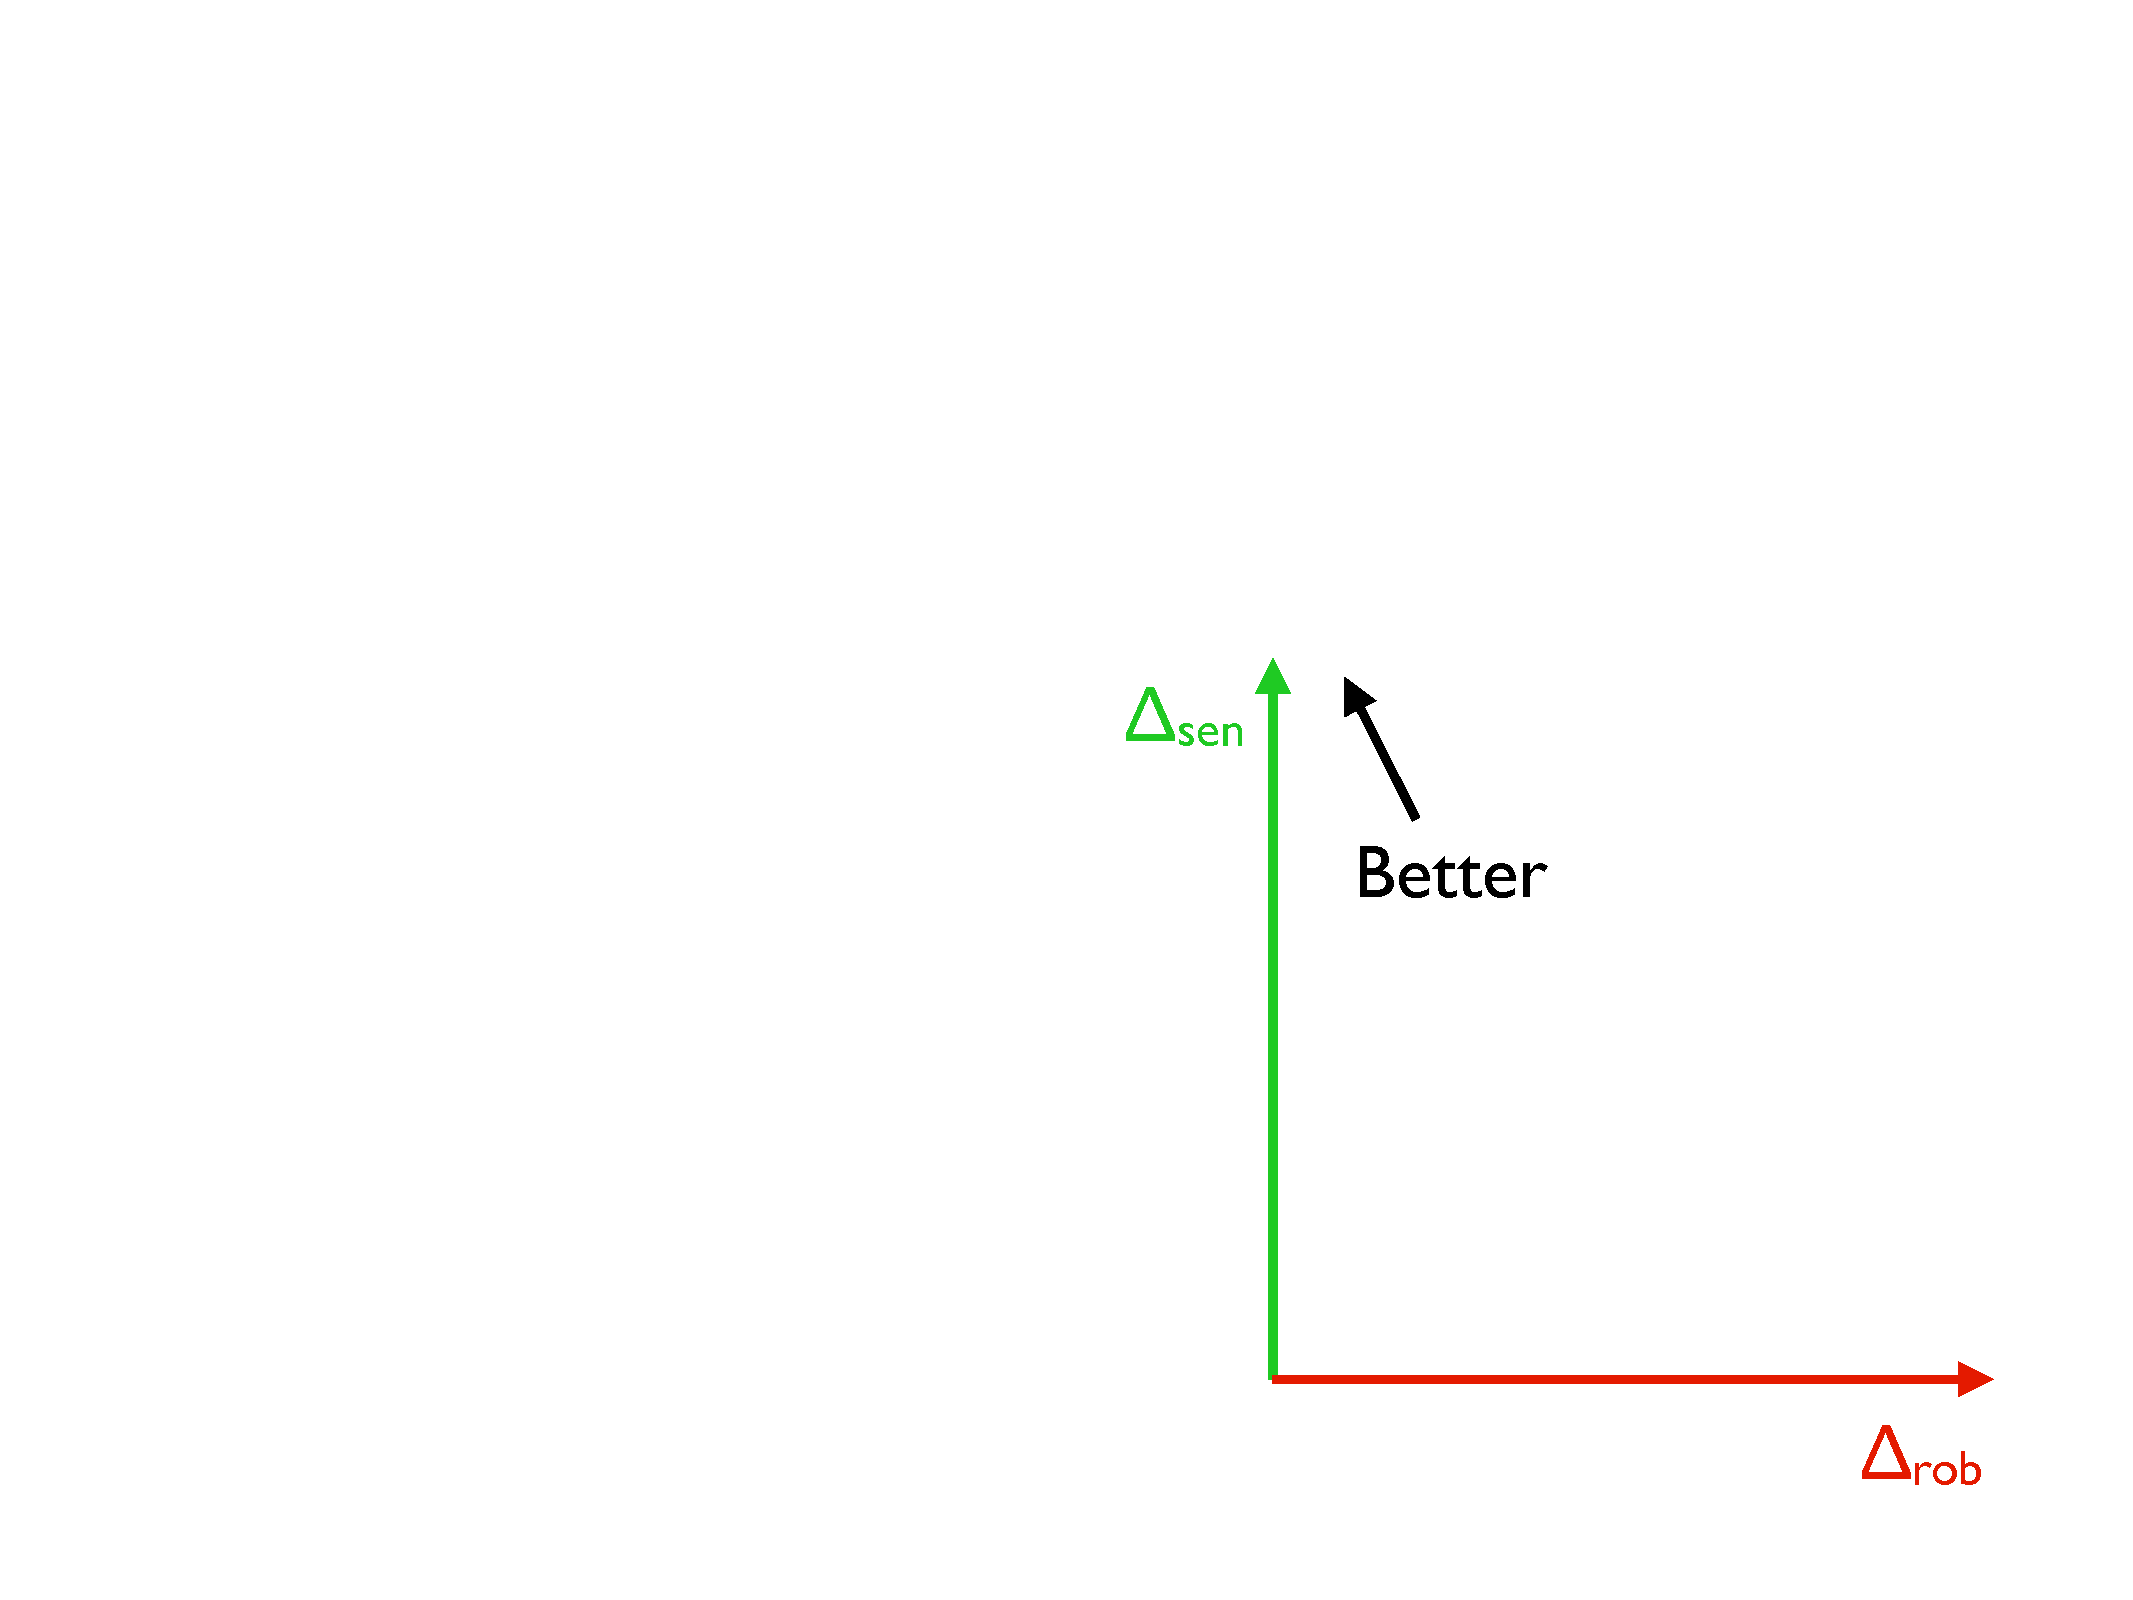
\includegraphics[width = 0.4\columnwidth]{figures/robustnessschematic.pdf}
\end{center}
\caption{A schematic diagram to illustrate the sensitivity-robustness plane defined by the separation power defined in Eq.~\ref{eq:seppower}.}
\label{fig:robustnessschematic}
\end{figure}

The sensitivity-robustness tradeoff is studied using (formally) leading logarithm PS MC programs \herwig.1~\cite{Bellm:2015jjp,Reichelt:2017hts} with the default tune and \pythia.223~\cite{Sjostrand:2006za,Sjostrand:2014zea} with the tune 4C (CONFIRM - Monash is default in 8.2).  Results are presented for separately for quark and gluon jets, using the $Z+q$ and $Z+g$ hard-scattering processes.  A variety of angularities (as defined in Sec.~\ref{sec:shape_def}) are studied, with $\alpha\in\{0.5,1.0, 2.0\}$ corresponding to the Les Houches Angularity~\cite{Gras:2017jty}, width, and mass, respectively.  Additionally, various grooming parameters are studied by varying $\beta\in\{0,1,2\}$ and $z_\text{cut}\in \{0.05,0.1,0.2\}$.  

\begin{figure}[h!]
\begin{center}
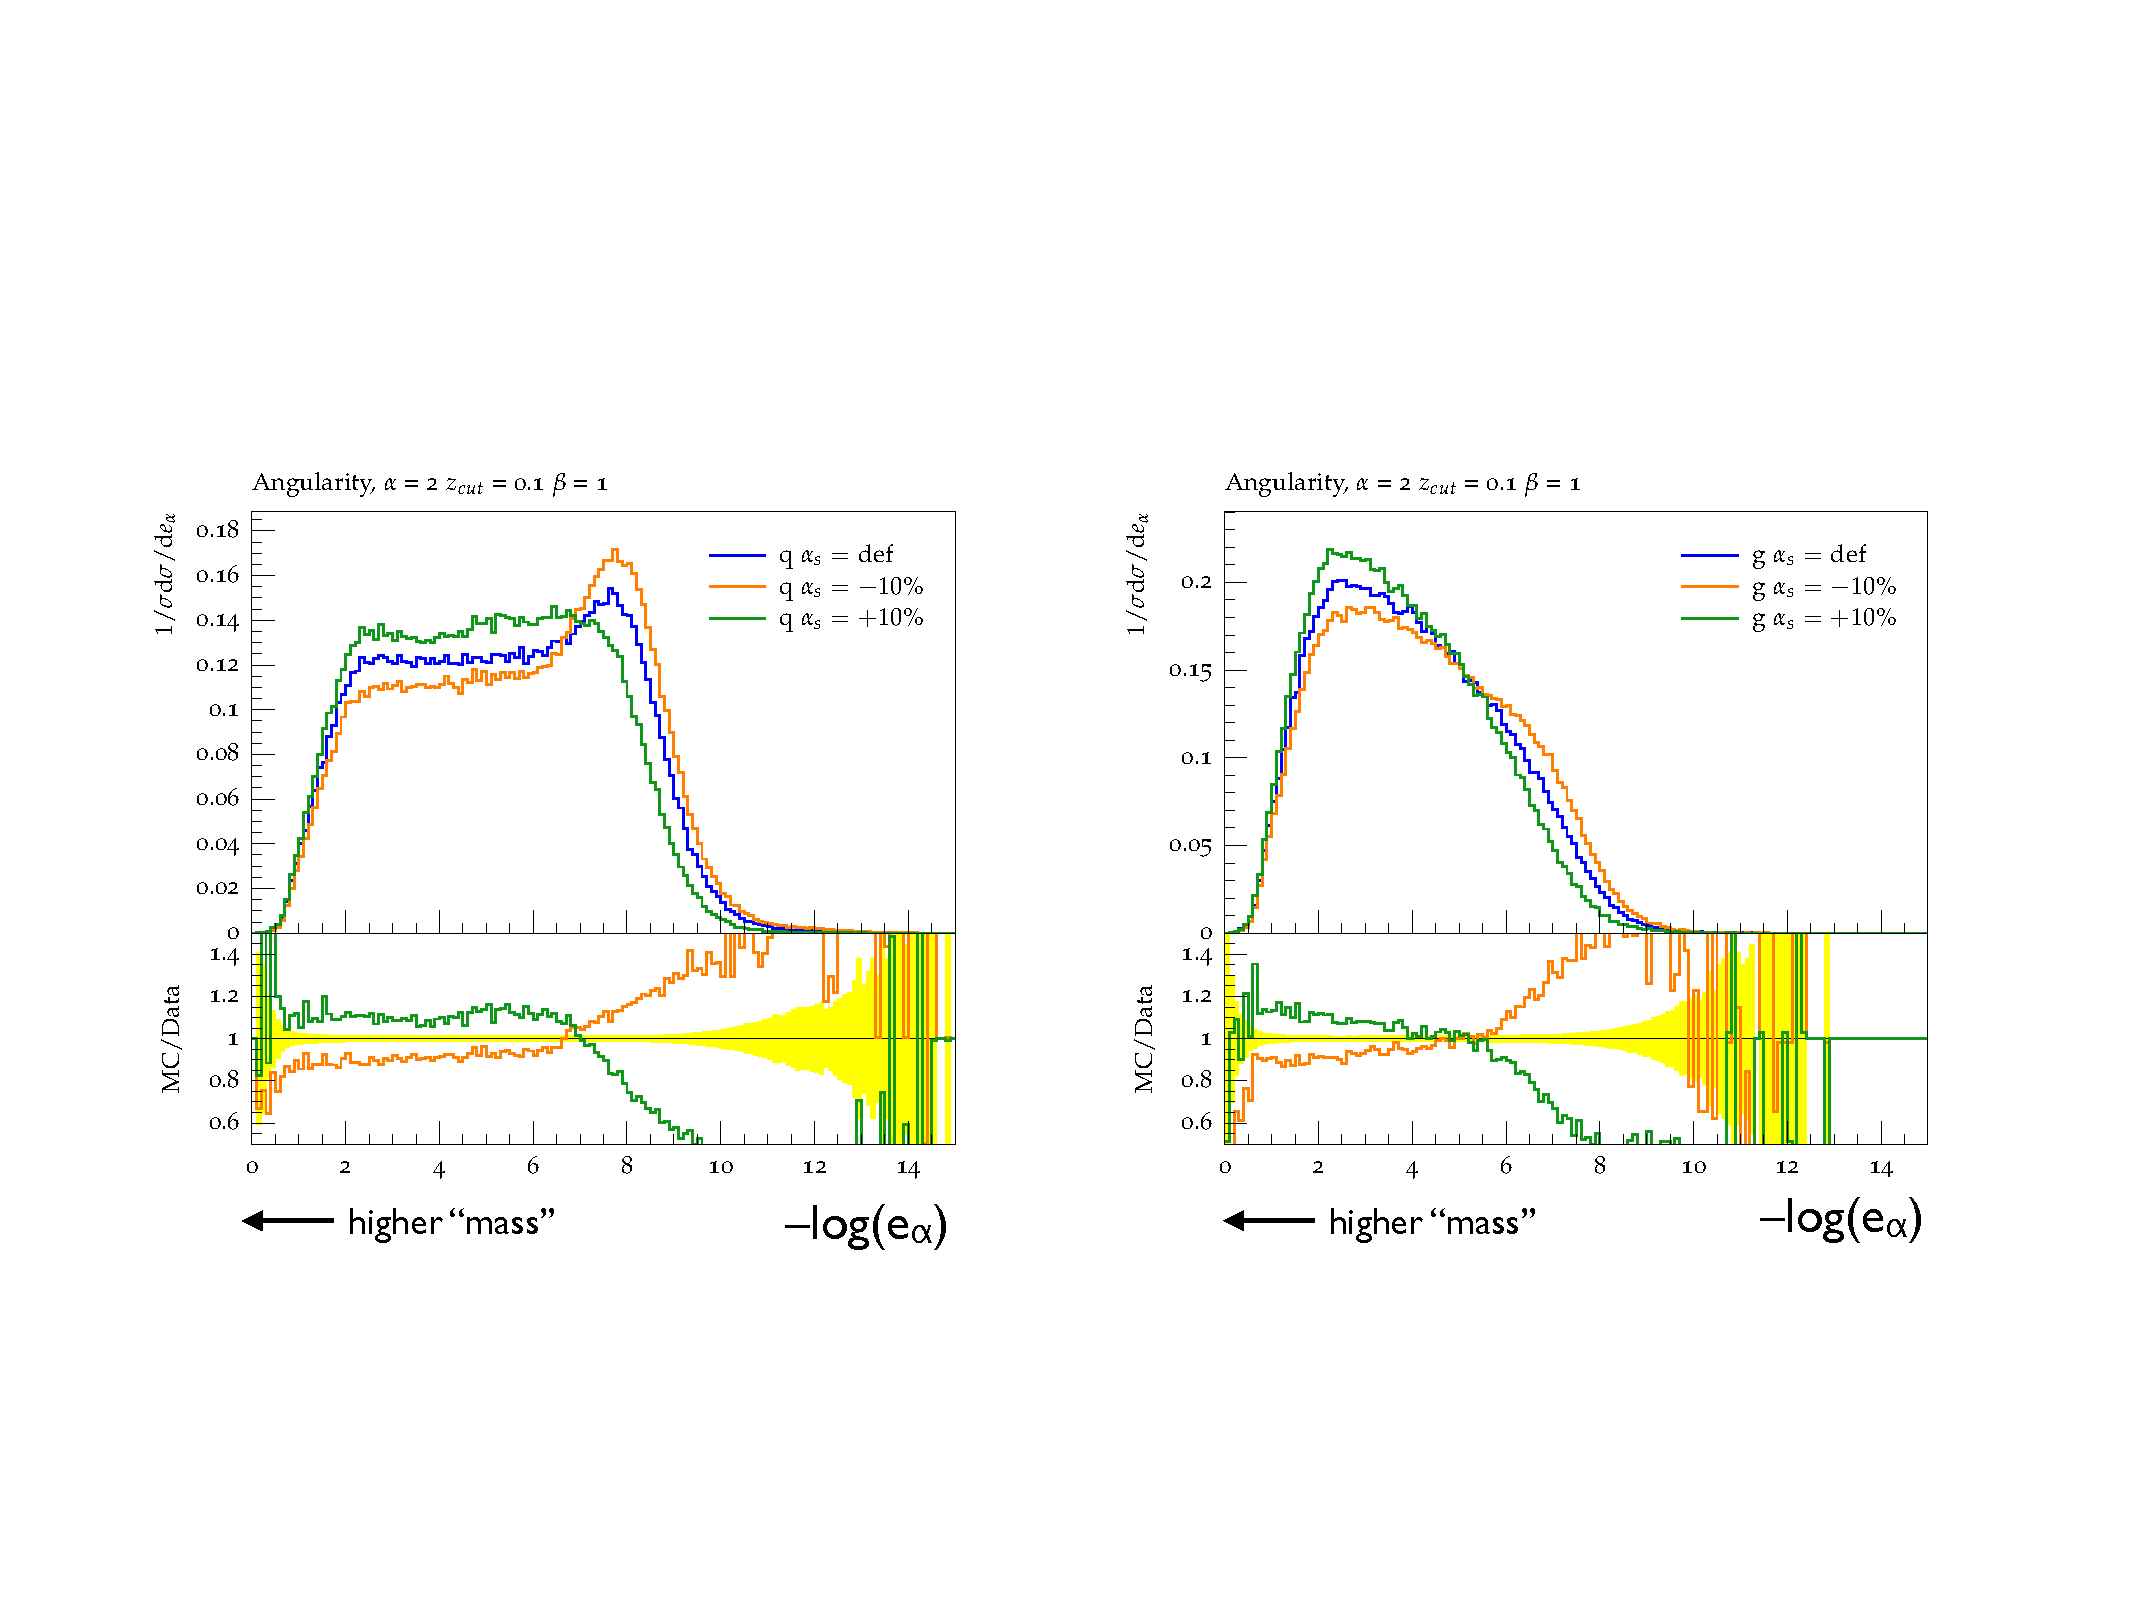
\includegraphics[width = 0.99\columnwidth]{figures/sensitivity.pdf}
\end{center}
\caption{The distribution of the normalized squared jet mass ($e_2$) for quark jets (left) and gluon jets (right).  Higher values of the mass are on the left.  The blue line uses $\alpha_s=0.118$ while the green and orange lines have the value of $\alpha_s$ varied by $10\%$.  The lower panels show the ratio with respect to the $\alpha_s=0.118$ curve.\textbf{Maybe cut the x-axis at high values?  Maybe comment what the picture looks like for Pythia?}}
\label{fig:sensitivity}
\end{figure}

\begin{figure}[h!]
\begin{center}
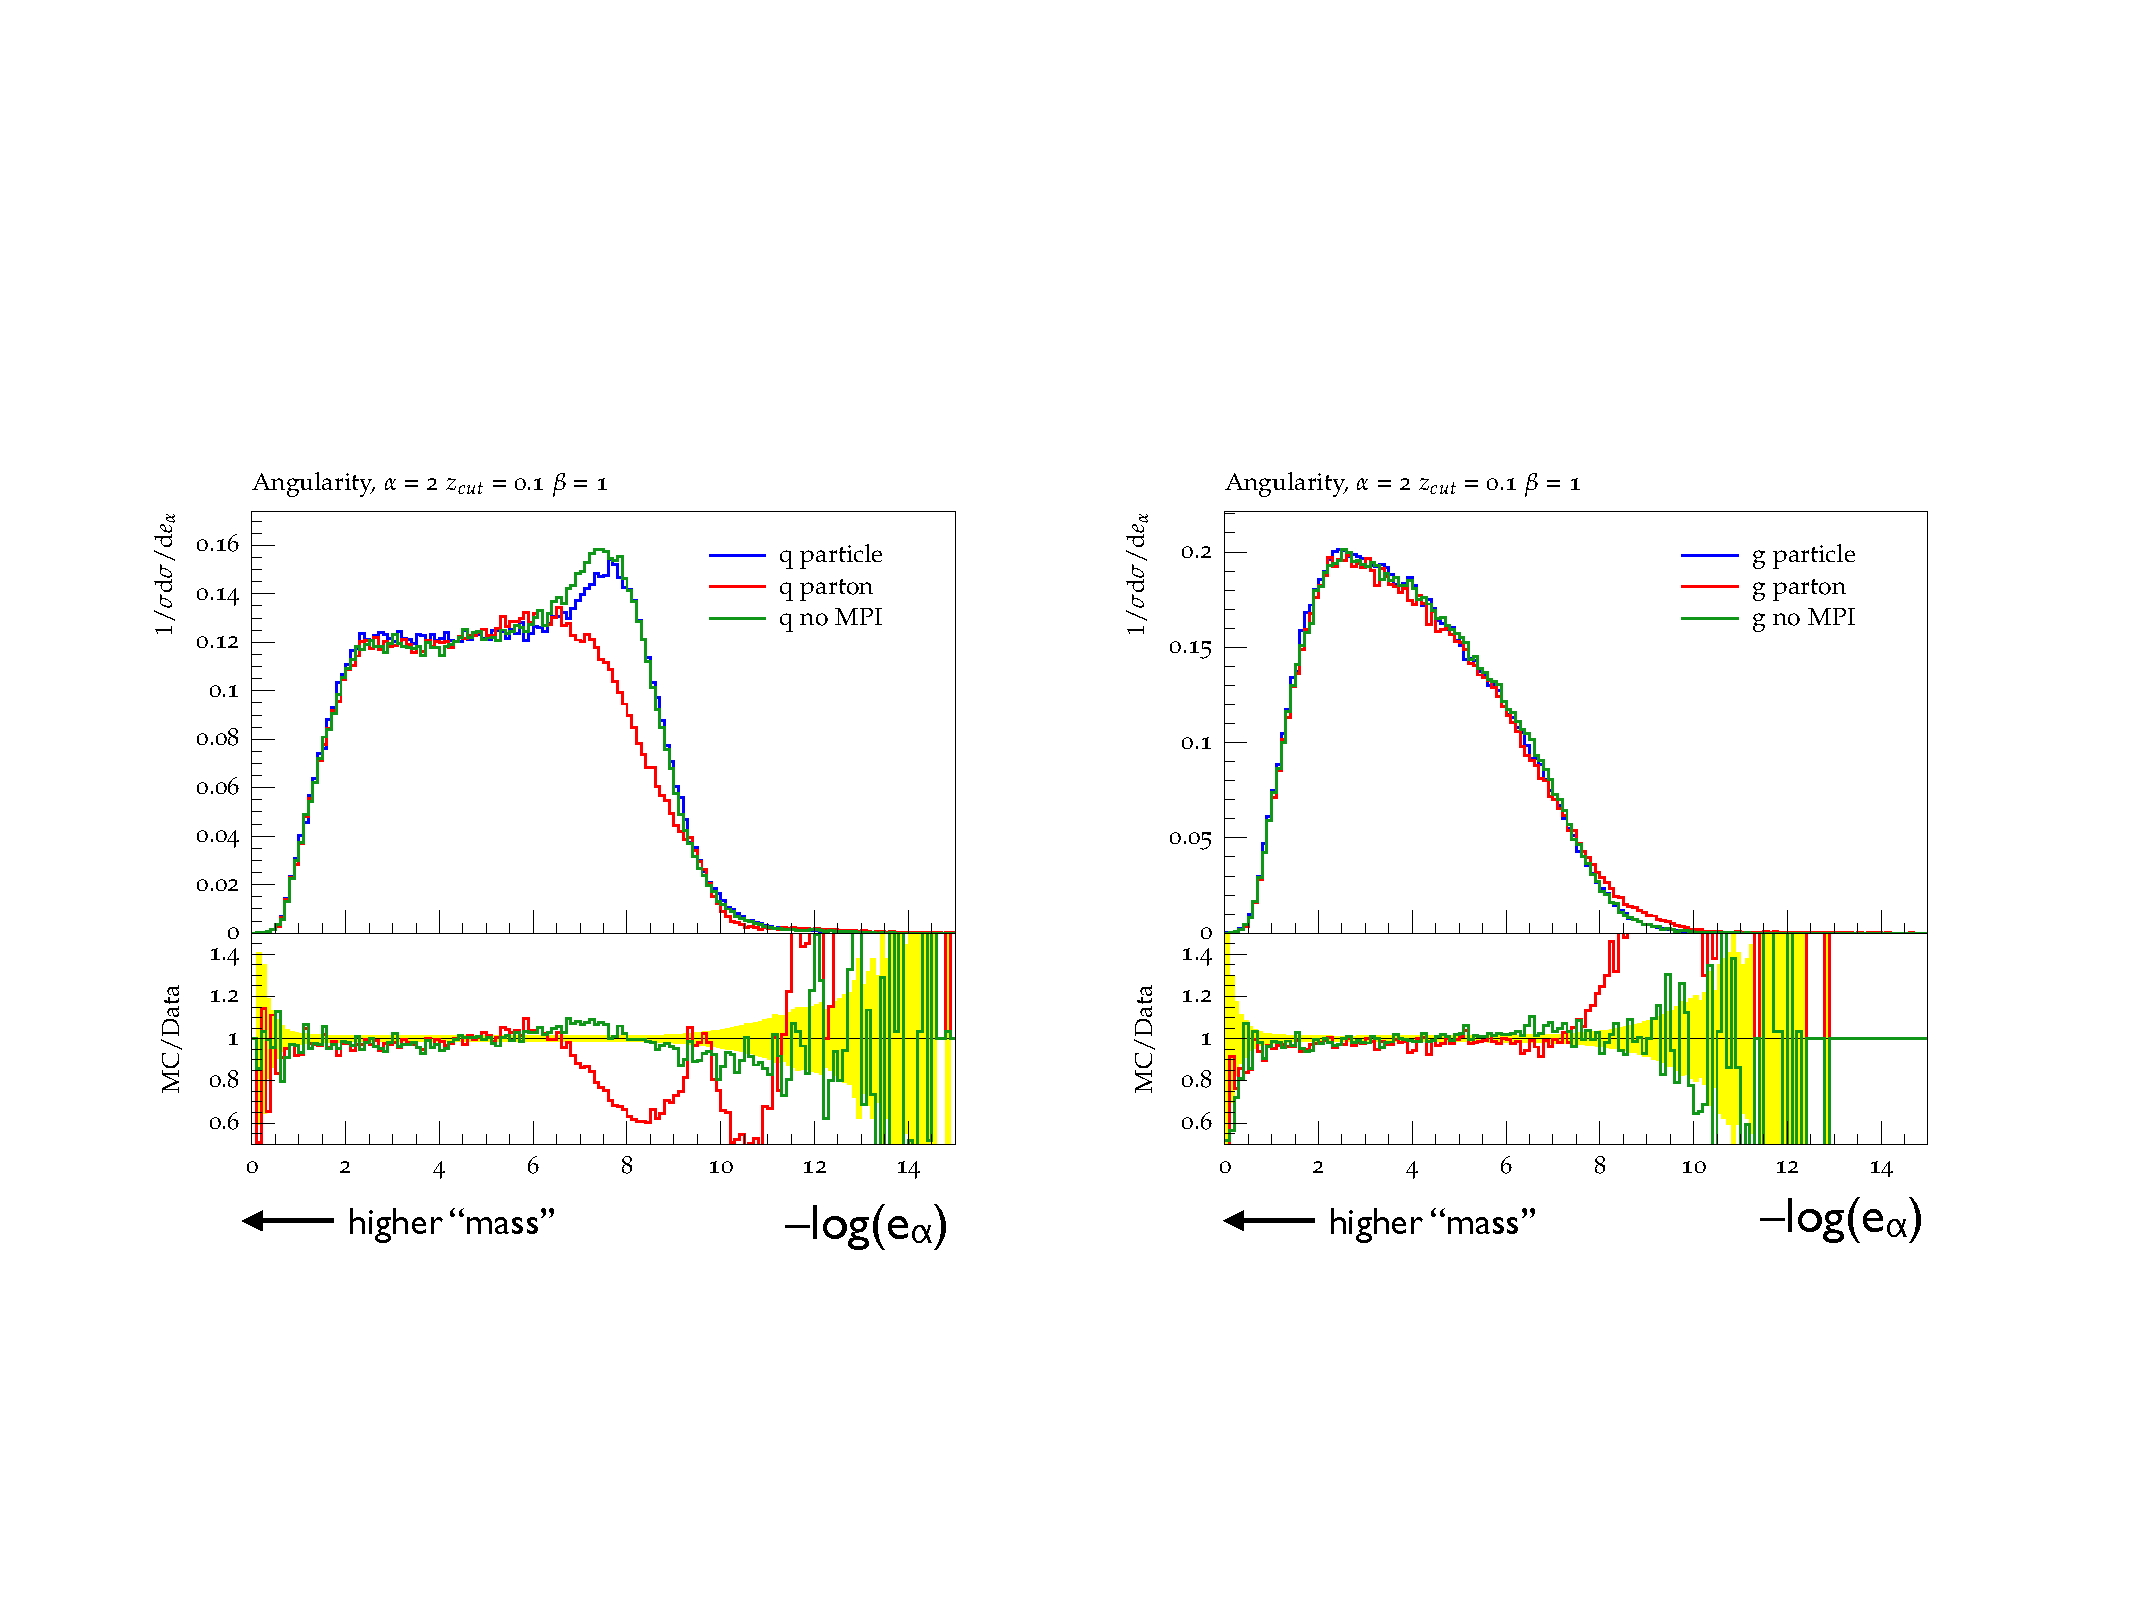
\includegraphics[width = 0.99\columnwidth]{figures/robustness.pdf}
\end{center}
\caption{The distribution of the normalized squared jet mass ($e_2$) for quark jets (left) and gluon jets (right).  Higher values of the mass are on the left.  The blue line shows the default particle-level simulation that includes the standard cluster hadronization model.  The red curve has hadronization turned off and the green curve is the same as the blue, but with the \herwig model for multiple parton interactions (MPI) turned off.  MPI is also off for the red curve.  \textbf{Maybe cut the x-axis at high values?  Maybe comment what the picture looks like for Pythia?}}
\label{fig:robustness}
\end{figure}

\begin{figure}[h!]
\begin{center}
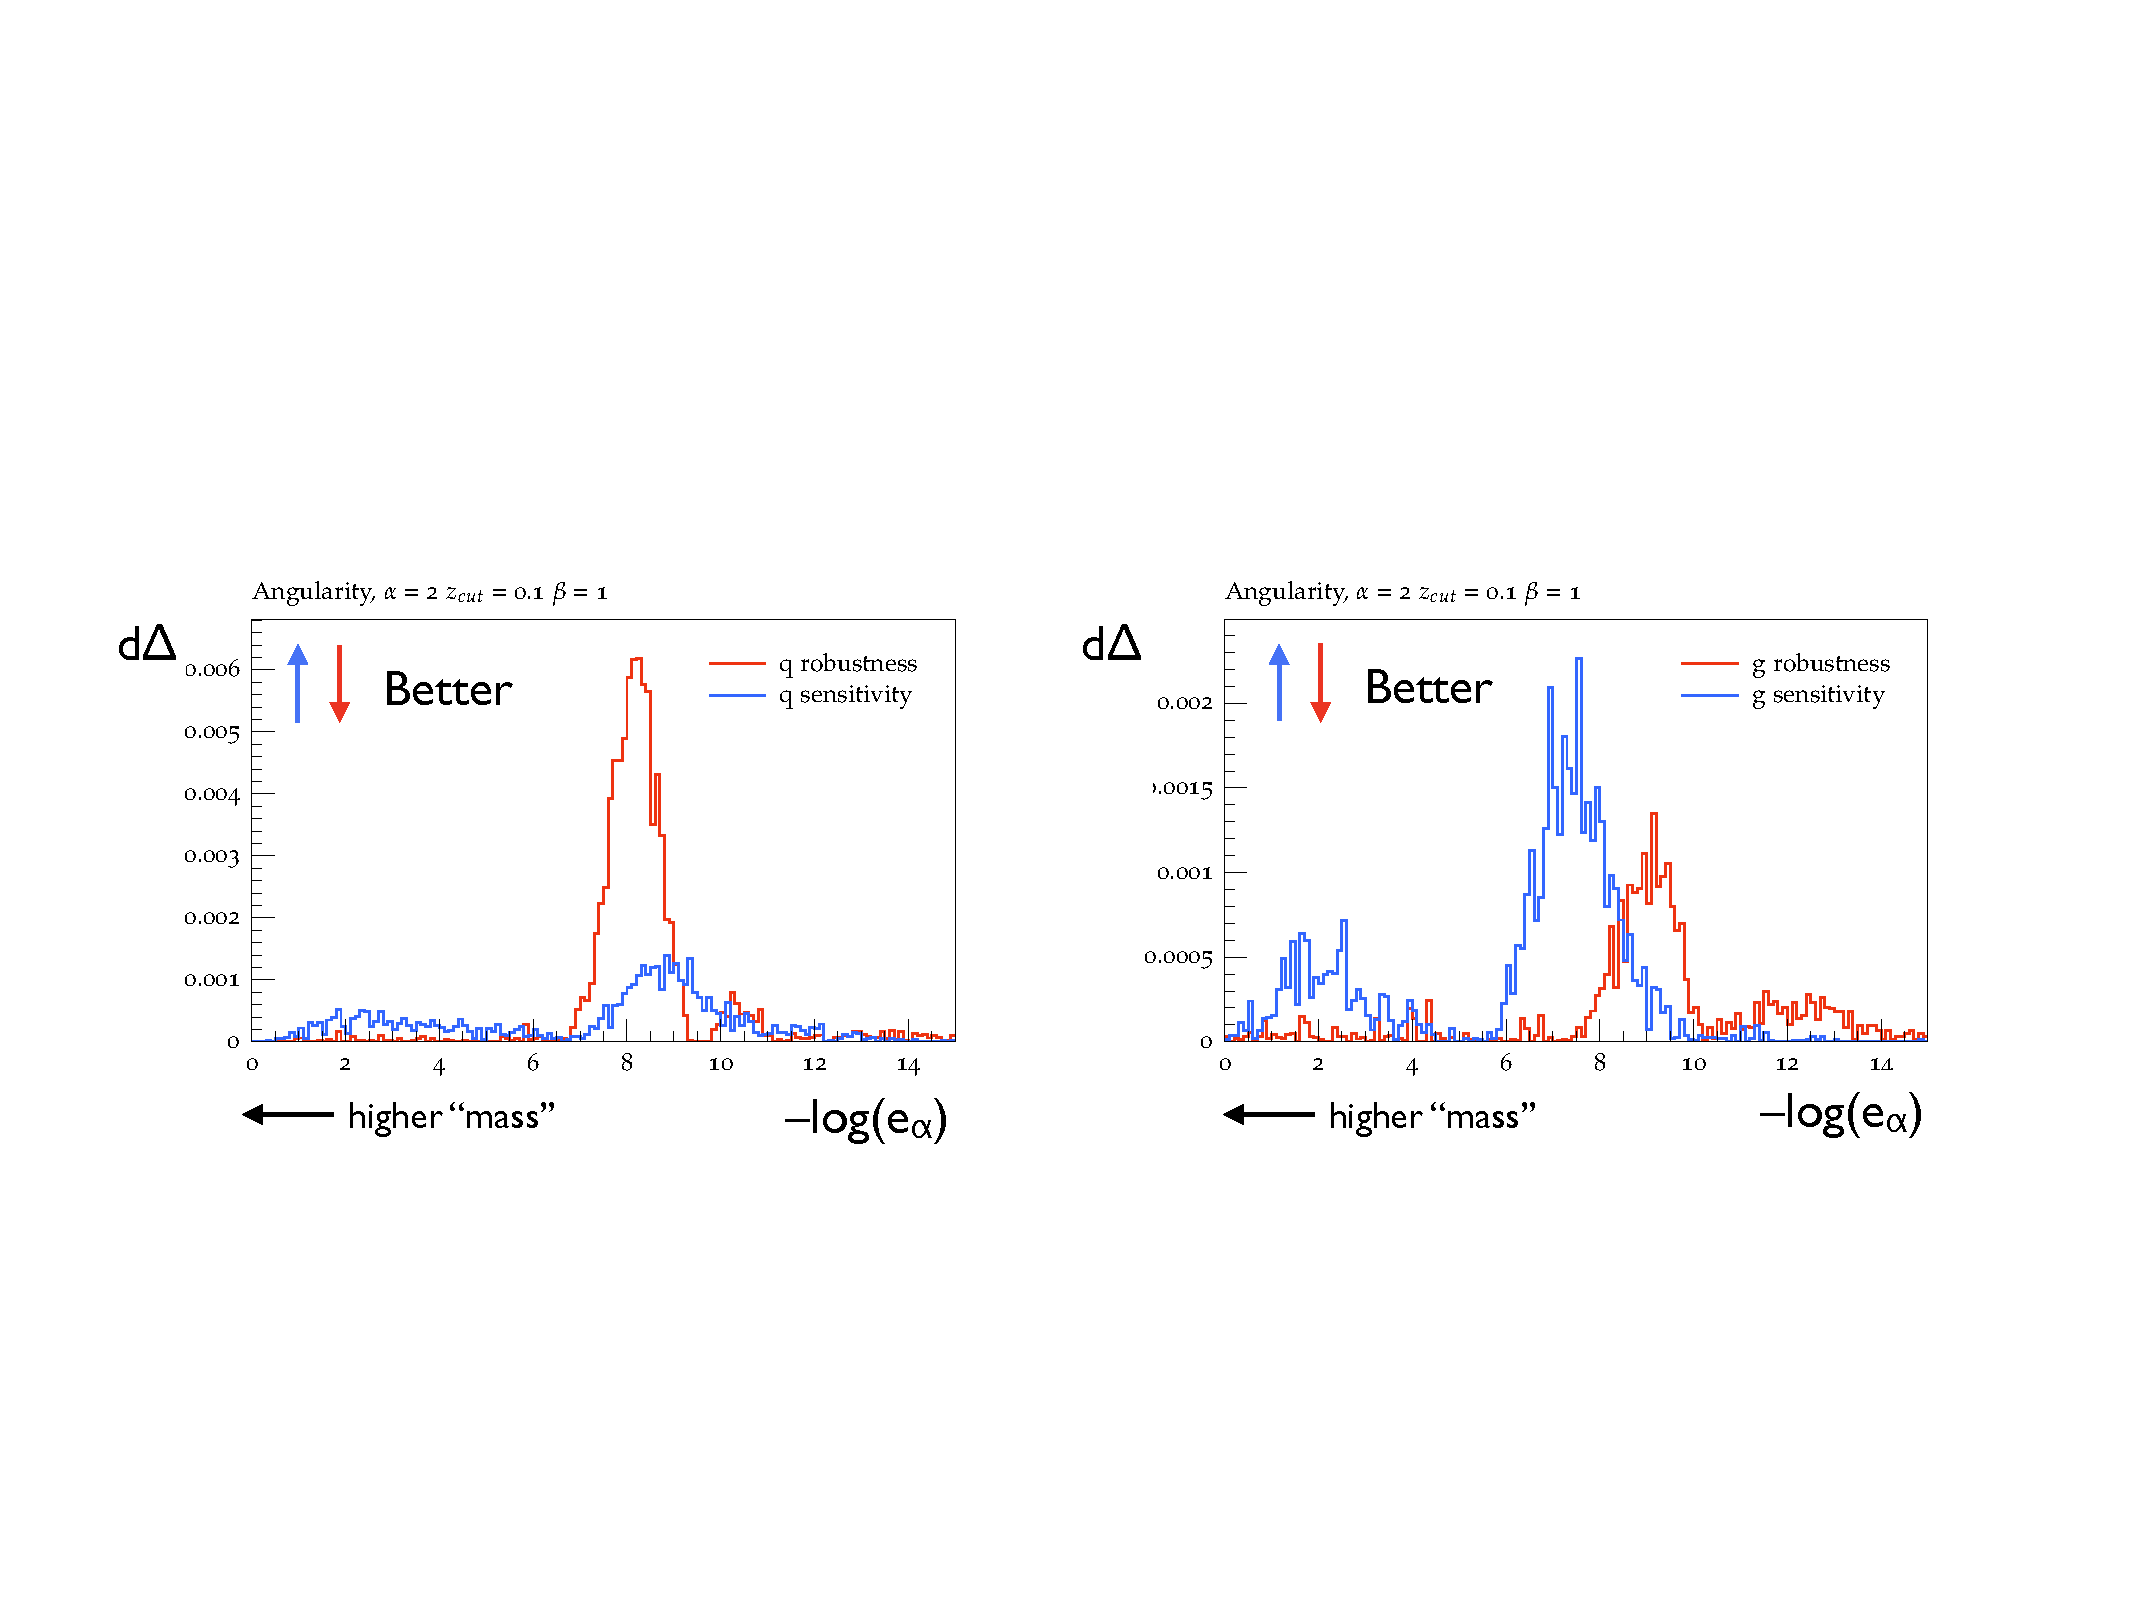
\includegraphics[width = 0.99\columnwidth]{figures/differentialseparation.pdf}
\end{center}
\caption{The integrand of Eq.~\ref{eq:seppower} for the normalized squared jet mass ($e_2$) for quark jets (left) and gluon jets (right).  Higher values of the mass are on the left.  In $f$ from Eq.~\ref{eq:seppower} is the same for red and blue, but for blue (sensitivity), $\alpha_s$ is varied by 10\% and for red (robustness), hadronization is turned off.}
\label{fig:differentialseparation}
\end{figure}

Figures~\ref{fig:sensitivity} and~\ref{fig:robustness} show the distribution of the normalized squared jet mass ($e_2$) for quark and gluon jets.  To the left of the low-mass peak, the shape of the $e_2$ distribution is nearly flat for quarks and nearly linear (in the log-space) for gluons.  Increasing $\alpha_s$ shifts the quark distribution up but has nearly no impact on the shape of the distribution below the peak.  The size of the peak is significantly impacted by the value of $\alpha_s$.  In contrast, the slope of the distribution for gluons changes with the variations in $\alpha_s$.  Figure~\ref{fig:sensitivity} shows the same $e_2$ distribution, but now with variations in the modeling of non-perturbative effects.  The low-mass peak for quarks is entirely due to hadronization effects.  According to the Herwig 7 MC, the impact of hadronization is much smaller for gluon jets.  Figure~\ref{fig:differentialseparation} shows the distribution of the differential separation power (integrand of Eq.~\ref{eq:seppower}), using the variation with $\alpha_s$ as the sensitivity and the change from turning off hadronization as the robustness.  For quark jets, Figs.~\ref{fig:sensitivity} and~\ref{fig:robustness} showed that the biggest variations with $\alpha_s$ occurred at low mass which is also where non-perturbative effects are largest.  This corresponds to the peak in the blue and red distributions in Fig.~\ref{fig:differentialseparation} occurring in nearly the same location.  In contrast, the peaks are more well-separated in Fig.~\ref{fig:differentialseparation} for gluon jets and the blue is shifted to higher mass values where there is more perturbative control.  

\begin{figure}[h!]
\begin{center}
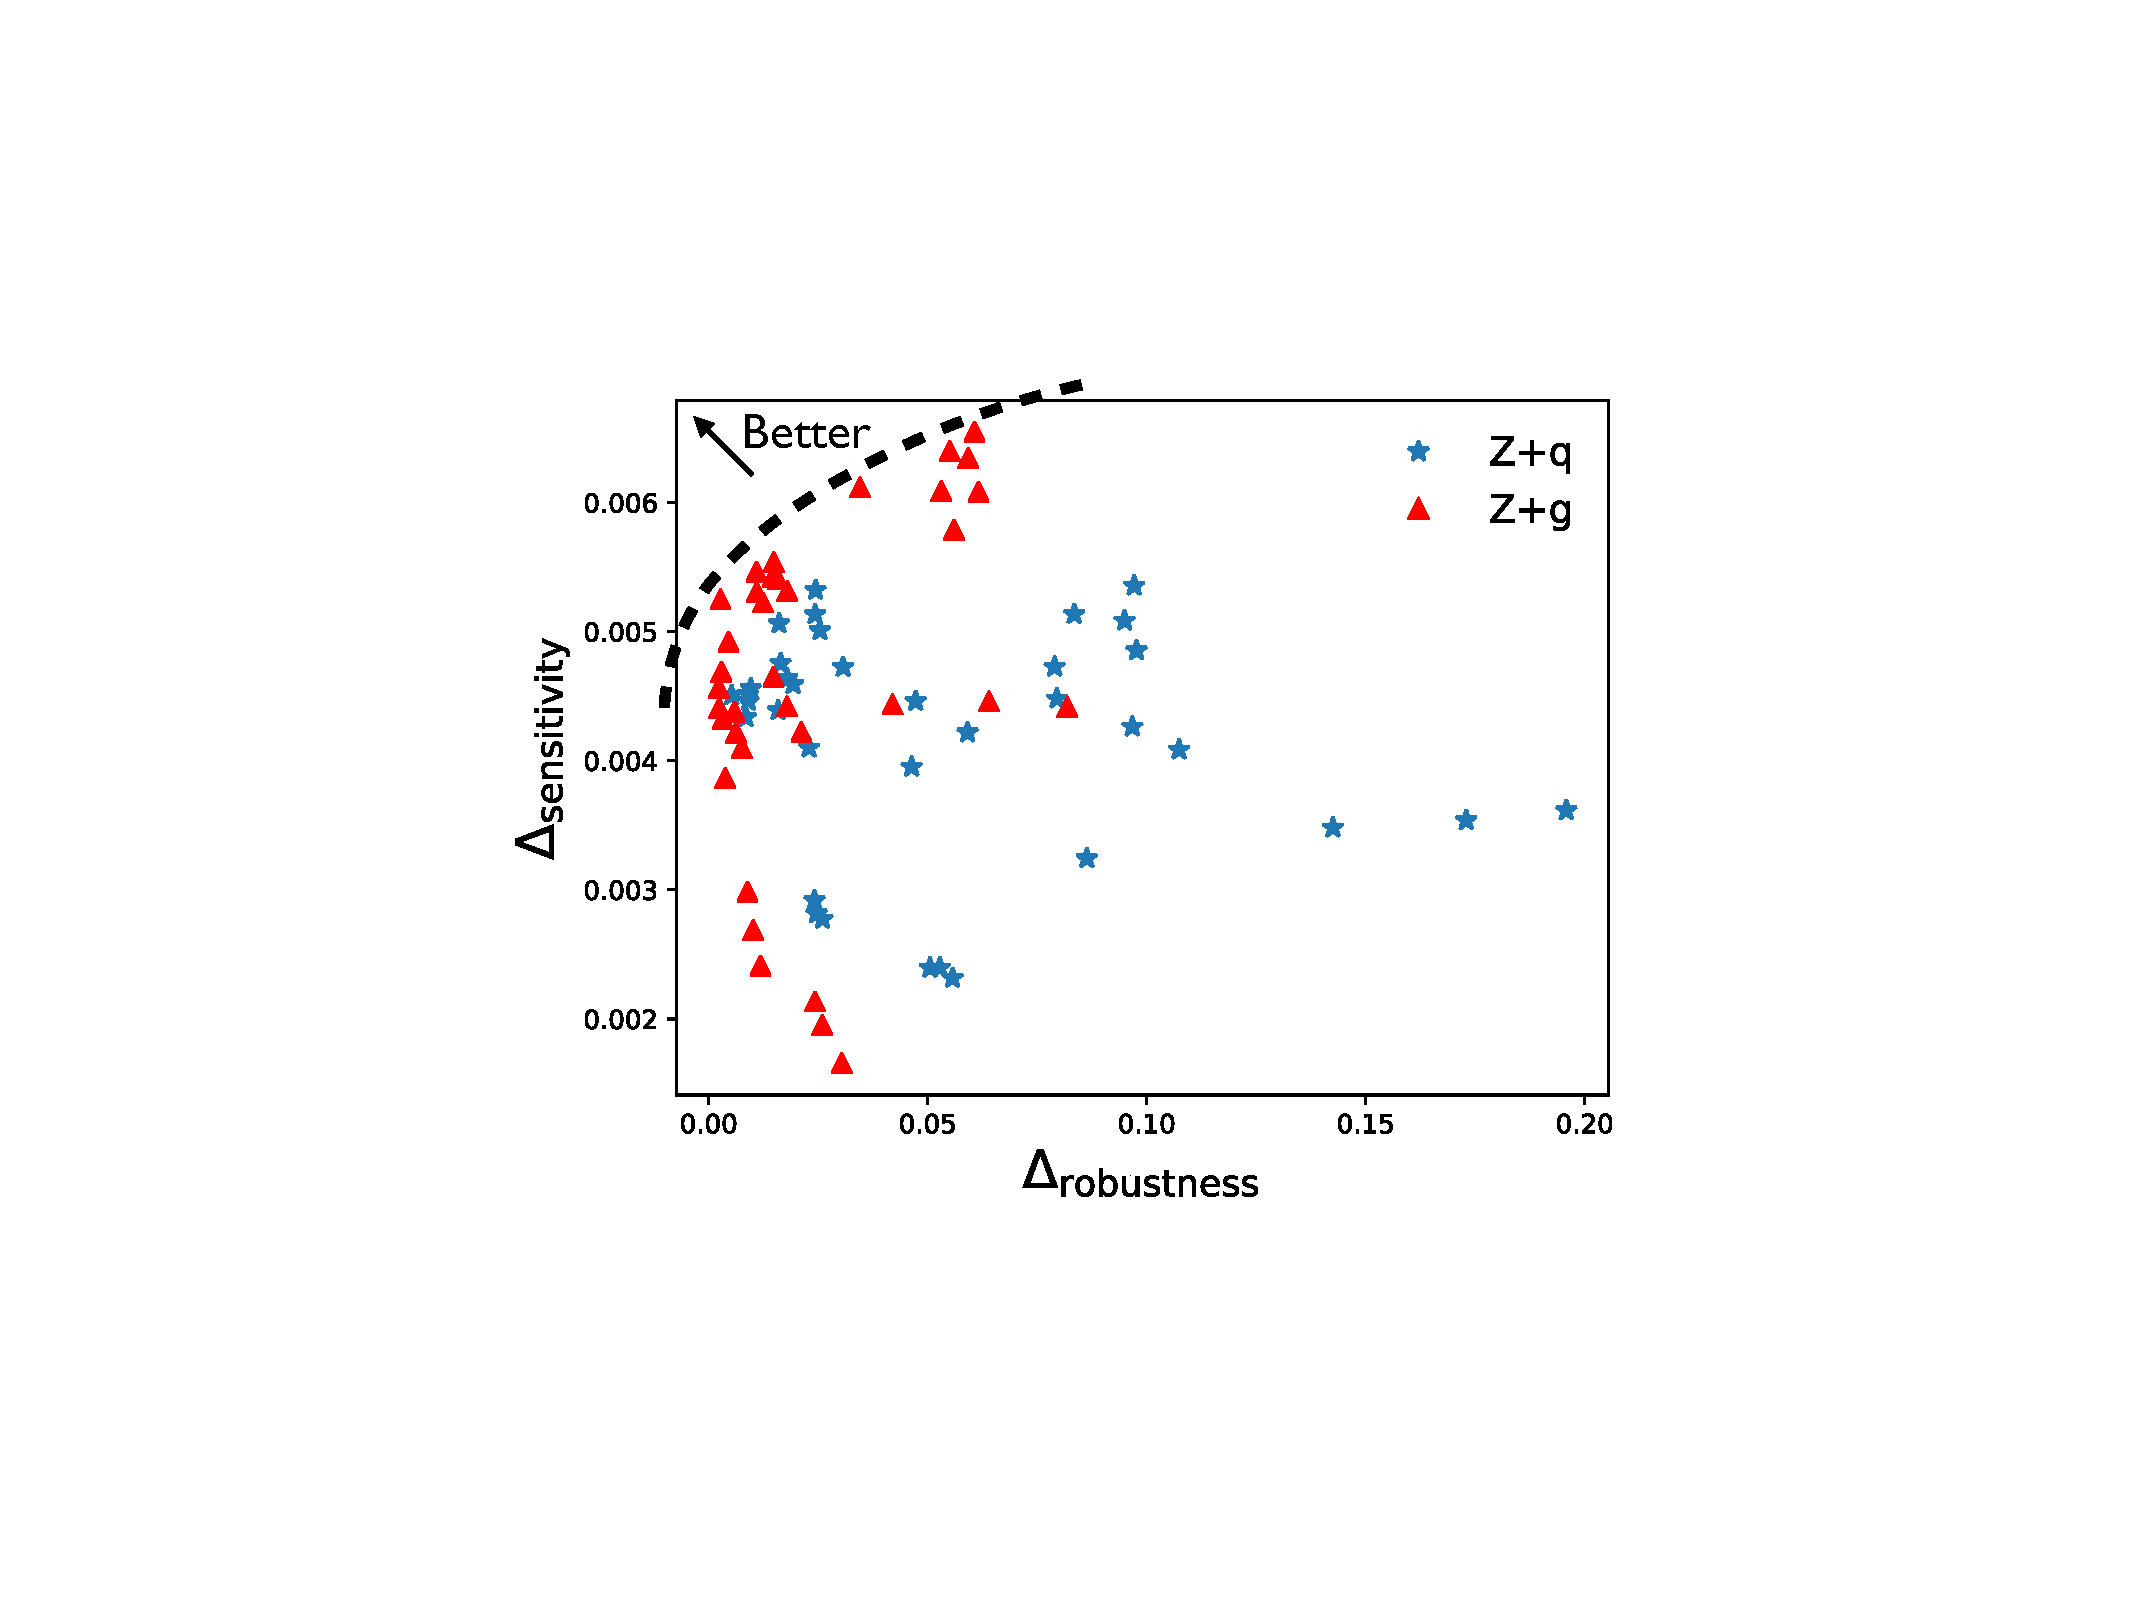
\includegraphics[width = 0.6\columnwidth]{figures/robseptradeoff.pdf}
\end{center}
\caption{The tradeoff between sensitivity and robustness for the 27 angularities studied in this section along with 27 $\theta_g$.  Stars represent quark jets and triangles represent gluon jets. \textbf{Should explain where 36 comes from (includes $\theta$).  How does this picture change if we truncate the range of $\lambda$?  (see Gregory's formula).}}
\label{fig:robseptradeoff}
\end{figure}

A summary of the sensitivity-robustness tradeoff for many angularities is presented in Fig.~\ref{fig:robseptradeoff}.  As already observed for the jet mass, gluons tend to have a superior sensitivity and robustness compared with quarks.  This is not surprising, as gluons have more perturbative radiation than quarks ($C_A>C_F$).  The jet mass has $(\Delta_\text{sensitivity},\Delta_\text{robustnes})=(?,?)$.  The angularities with the highest quark and gluon sensitivity and robustness are ?, ?, and ?.   Conclusion + transition sentence(s).

The usual mass (zcut = 0.1, beta = 0, alpha = 2, which is 33) is pretty good for gluons but not very good for quarks.  The best configurations seem to be 19 and 20.  These correspond to alpha = 1, zcut = 0.05, and beta = 1 or 2.  This is like kT with different grooming parameters so is maybe not so surprising as the scale of alphas is set by kT.  Seems to also have better robustness.  Would it be possible to get the Fig. 5-7 versions of those?  Might be worth including or at least putting in an appendix.  (also interesting that the version with beta = 0 is strictly much worse, in these metrics).








%%%%%%%%%%%%%%%%%%%%%%%%%%%
\subsection{The Issue of Casimir Scaling}
\label{sec:casimir}
%%%%%%%%%%%%%%%%%%%%%%%%%%%



While we have illustrated that the groomed jet mass observable provides a sensitivity to $\alpha_s$ particularly for gluon jets, one problem that is immediately clear from \Sec{sec:analytic} is that the leading behavior of the distributions is always dominated by the product $\alpha_s C_i$. While this is broken at higher perturbative orders, it implies that at lowest order there is a complete degeneracy of the value of $\alpha_s$ and the quark vs. gluon fraction of jets. This problem is not faced at $e^+e^-$ colliders.

There are a variety of different approaches to overcome this problem, each with their own advantages and disadvantages. First, we note that the quark and gluon fractions are perturbatively calculable given the Parton Distribution Functions (PDFs). Therefore, perturbatively calculating the quark and gluon fractions inputs the most possible information, and should correspondingly lead to the best sensitivity for $\alpha_s$. However, it has the downside that it also introduces sensitivity to the PDFs, which in principle should be fitted along with $\alpha_s$~\cite{Accardi:2016ndt}. This difficulty also enters into other extractions at the LHC, for example the $3$-$2$ jet rate or the EEC. However, a hope of using jet substructure was that the sensitivity to the PDFs could be minimized.

A second approach is to simultaneously fit for the quark (or gluon) fraction. Due to the fact that the two fractions must add to unity, this introduces a single additional parameter (see Fig.~\ref{fig:analyticbanana}). The degeneracy between the quark and gluon fraction and $\alpha_s$ is broken by higher order effects. Furthermore, different $\ecf{2}{\alpha}$ have different dependence on $\alpha_s$ and $C_i$ at higher orders. Therefore, the measurement of multiple angularities would allow the degeneracy to be broken. However, from a theoretical perspective, this significantly complicates the analysis, and we do not believe that precise predictions will be made in the near future, except for $\alpha=2$, and perhaps $\alpha=1$. In our study in \Sec{sec:ben_study} we will consider both approaches.

It would be interesting to develop other approaches to disentangling the quark and gluon fractions and $\alpha_s$, however, we expect that this will be a limiting aspect of $\alpha_s$ extractions at the LHC.


\begin{figure}[h!]
\begin{center}
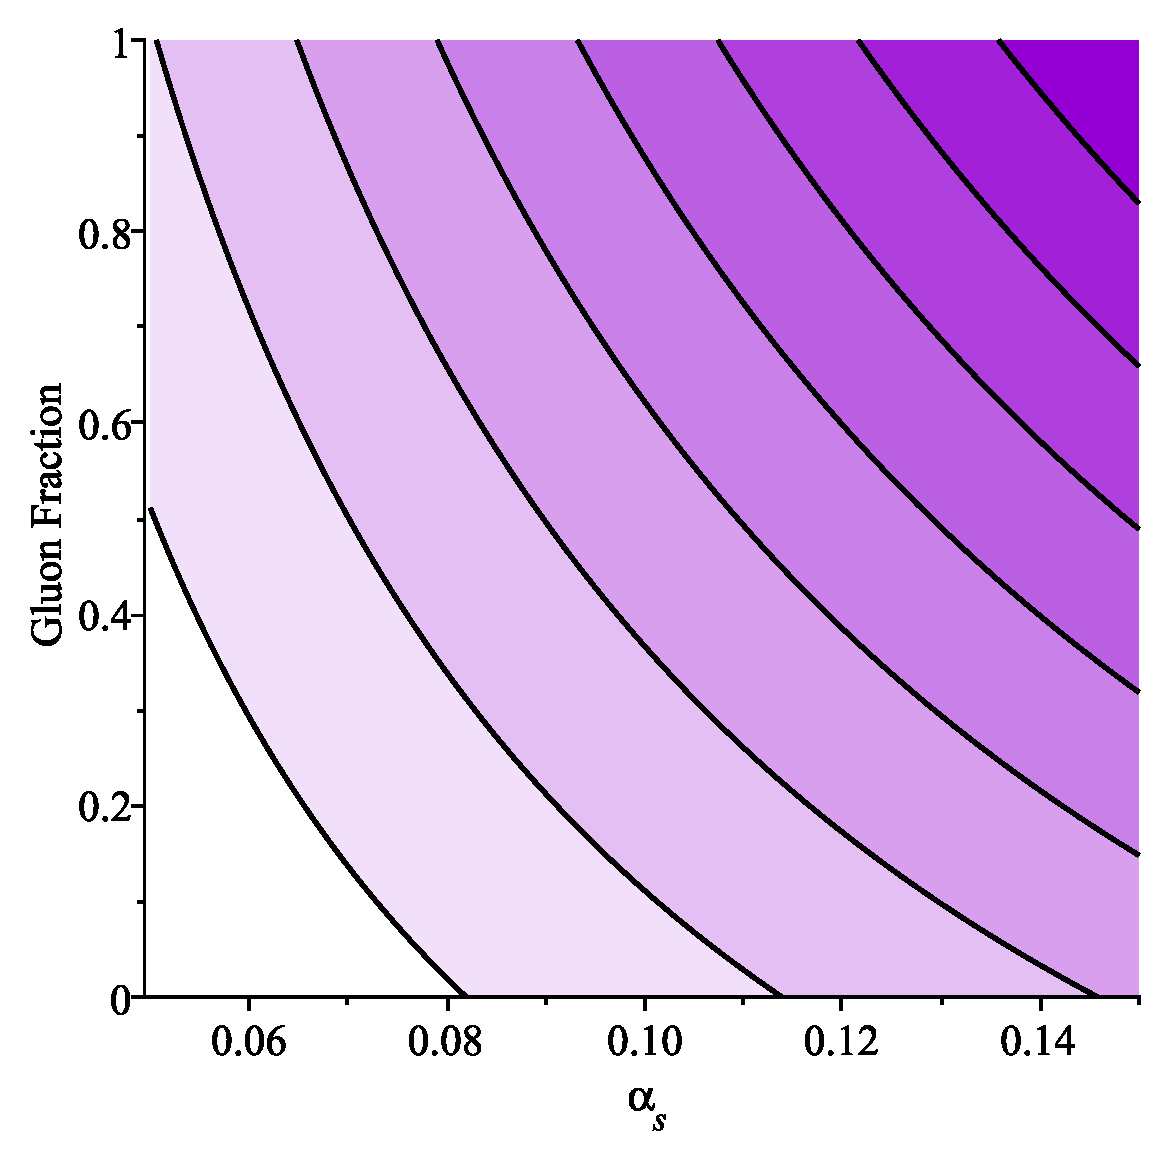
\includegraphics[width = 0.4\columnwidth]{figures/Degeneracy}
\end{center}
\caption{The slope of the probability distribution of $\ecf{2}{2}$ (as a function of $\log(\ecf{2}{2})$) is proportional to $\alpha_s(C_Af_g+C_F(1-f_g))$, which is plotted above.  The degeneracy between $\alpha_s$ and $f_g$ (gluon fraction) are represented by the banana-shaped isocontours. }
\label{fig:analyticbanana}
\end{figure}


%%%%%%%%%%%%%%%%%%%%%%%%%%%
\subsection{Normalized vs. Unnormalized Distributions}
%%%%%%%%%%%%%%%%%%%%%%%%%%%

In addition to the complication of quark and gluon fractions, another issue which appears for the extraction of $\alpha_s$ from jet substructure, as compared to $e^+e^-$ event shapes is the issue of normalization.\footnote{We thank Gavin Salam for interesting discussions regarding the issue of normalization.} Unlike in $e^+e^-$, the Born dijet cross section in $pp$ is sensitive to the value of $\alpha_s$. This implies that the rate itself, in particular, the absolute quark and gluon jet rates carries information regarding $\alpha_s$. 

Here we will focus on using the normalized distribution. We do this for three reasons. First, we would like this to be a true measurement of $\alpha_s$ from the jet substructure, and not be dominated by the overall rate. Second, and more importantly, it is currently only possible to perform the experimental measurement of the groomed mass precisely for the normalized distribution.  Experimentally, the absolute rate is determined by the acceptance from kinematic requirements on the jet $p_\text{T}$.  The sophisticated in-situ jet energy scale and resolution program carried out for small-radius jets~\cite{Aad:2014bia,Aaboud:2017jcu,Khachatryan:2016kdb,CMS-DP-2016-020} has not yet reached the same level of maturity for groomed large-radius jets.  However, this is simply a matter of time and efforts have already started in this direction~\cite{ATLAS-CONF-2017-063}.  A key challenge that still remains is to fully understand the correlations in the calibrations and uncertainties between the jet energy and the jet substructure observables.  Finally, the use of normalized distributions minimizes the sensitivity to the parton distribution functions.  As discussed in Sec.~\ref{sec:pertsimplicity}, grooming renders the quark and gluon angularity distributions universal.  Therefore, the measured distribution only depends on the fraction of gluon jets $f_g$ that pass the event selection.  In contrast, the total cross-section depends on the relative proportions of all possible partonic initial states.  This introduces a source of uncertainty that is not present for the normalized cross-section.  For example, the initial state could be one of $qq$, $qg$ or $gg$.  The relative proportions can be parameterized by two numbers $f_{qg}$ and $f_{gg}$ where $f_{qg}+f_{gg}=1-f_{qq}$.   Figure~\ref{fig:pdf} shows the uncertainty in the $f_{qg}$ and $f_{gg}$ from leading order PDFs.  Fixing $f_g$, which carries all of the PDF sensitivity for the shape measurement, has little effect on the uncertainty in $f_{qg}$ and $f_{gg}$.  This results in the residual PDF sensitivity from also measuring the total cross-section in addition to the shape of the angularity distribution.





One issue with using purely the normalized jet shape is that since the mass distribution starts at $\cO(\alpha_s)$. In other words, the slope of the groomed mass distribution is $\cO(\alpha_s)$. This implies that to have an $\cO(\alpha_s^2)$ uncertainty on the slope, one should have an NNLO calculation for a jet with two constituents.  In particular, this requires $2\to 3$ matrix elements. For the case of $e^+e^-$ this level of accuracy has been achieved, where the NNLO corrections to $e^+e^-\to 3$ jets are known, and are used in the extractions of $\alpha_s$. Due to recent progress in the calculation of the relevant amplitudes, we believe this is realistic.



\begin{figure}[h!]
\begin{center}
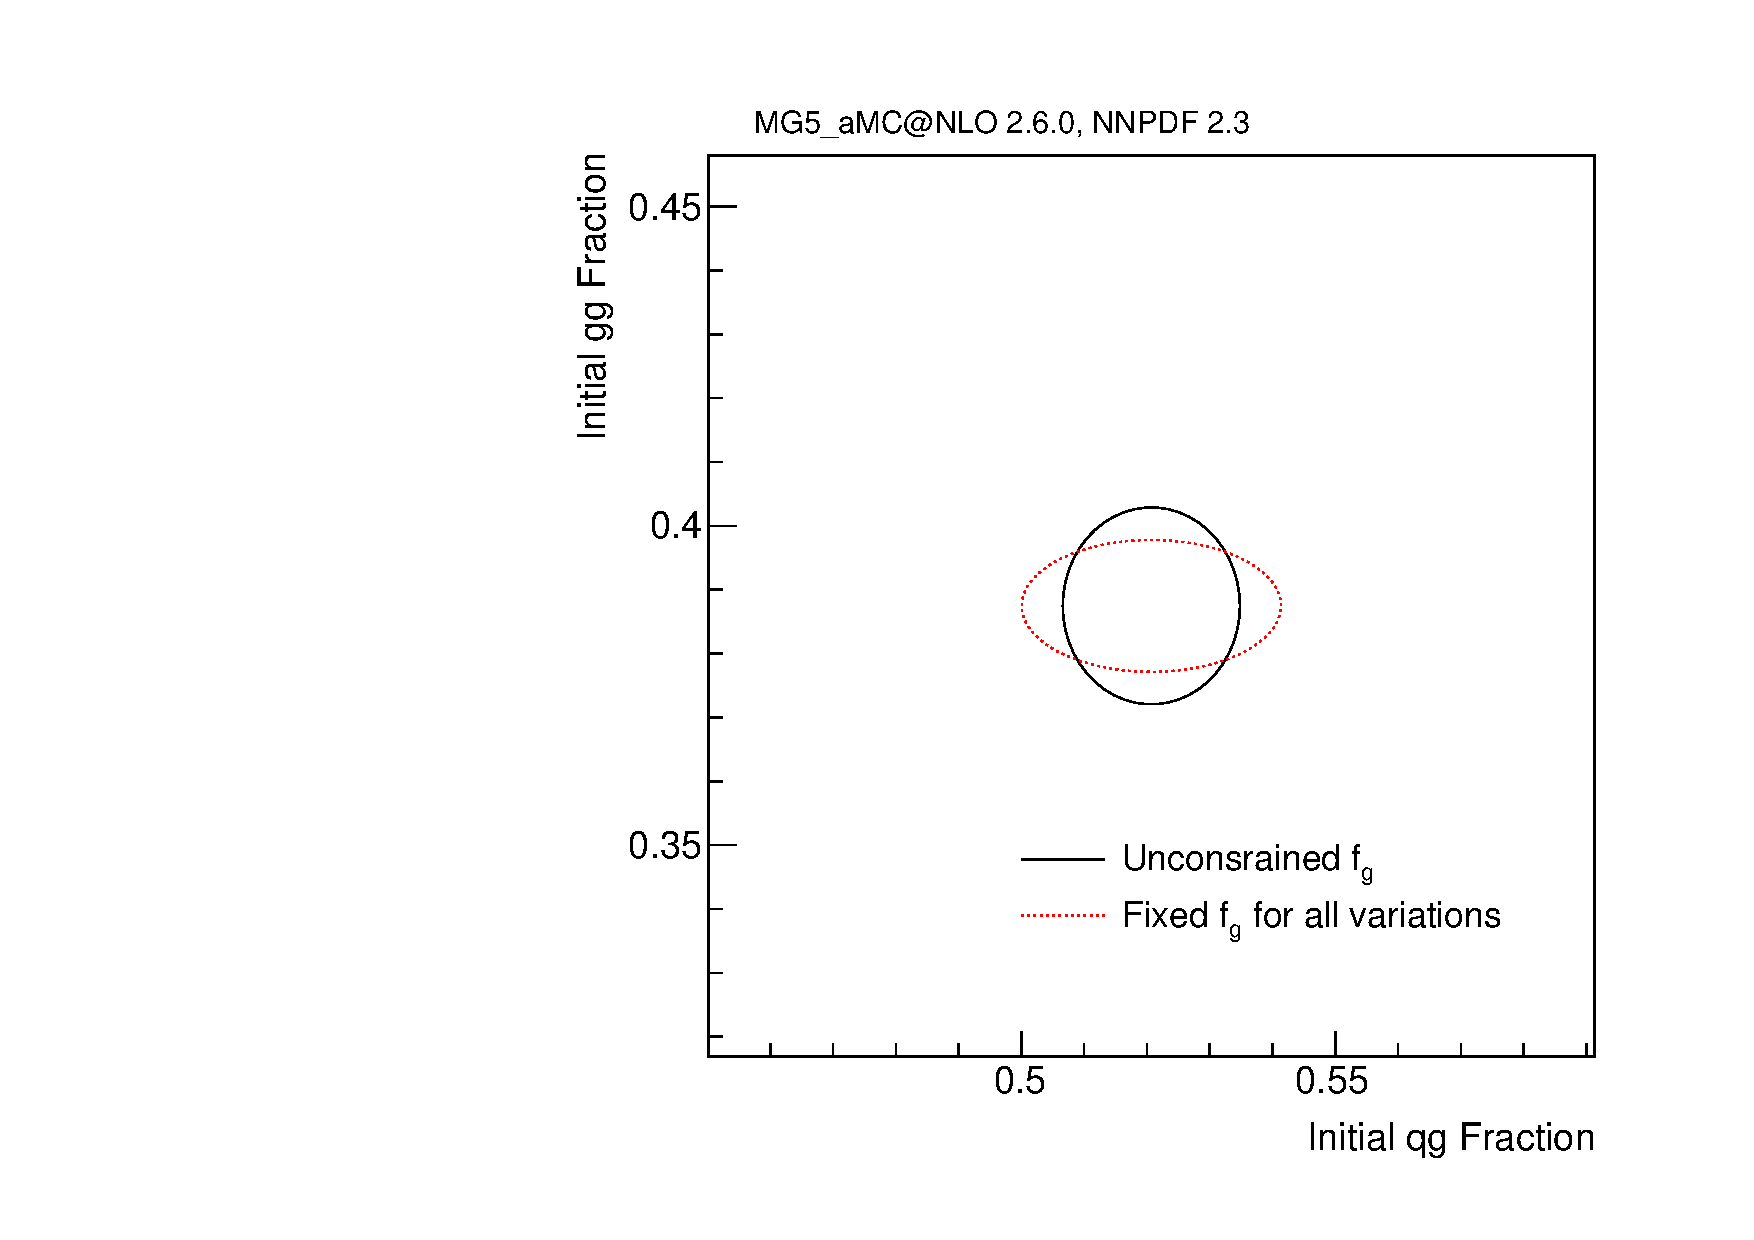
\includegraphics[width = 0.5\columnwidth]{figures/PDFs.pdf}
\end{center}
\caption{The fraction of $qg$ and $gg$ initial states for leading order dijet production simulated at leading order with MG5\_aMC 2.6.0~\cite{Alwall:2014hca} using the NNPDF 2.3~\cite{Ball:2012cx} parton distribution function (PDF) set.  The ellipses correspond to the uncertainty from the 100 error PDF sets.  For the red dashed line, the fraction of out-going gluon jets $f_g$ is constrained to be the same for all variations (and equal to the nominal PDF set).}
\label{fig:pdf}
\end{figure}





























%%%%%%


\clearpage

%%==============
\section{Idealized Performance at the LHC}
\label{sec:ben_study}
%%==============

%\info{Ben, Andrzej, Jesse, Gregory, Grigorios, Frederic}

The purpose of this section is to make some numerical estimates regarding $\alpha_s$ extraction from jet substructure at the LHC.
%
Many simplifying assumptions are made, with the goal of motivating a more complete effort within the context of ATLAS and CMS in collaboration with theorists.
%
First, we illustrate how $\alpha_s$ and the gluon fraction can be simultaneously extracted from the distribution of various two-point correlators.
%
Next, we estimate the needed experimental precision required to make a useful measurement of $\alpha_s$.
%
While both the theory and experimental precision will continue to improve over the next years, the community has already demonstrated that the work can begin with the first round of groomed jet mass results~\cite{Aaboud:2017qwh,CMS-PAS-SMP-16-010,Frye:2016aiz,Frye:2016okc,Marzani:2017mva,Marzani:2017kqd}.

\subsection{Extraction of Theory Templates}
\label{sec:templates}

A complete extraction of $\alpha_s$ will require matching resummed results to high fixed order and also estimating NP effects.
%
The two sets of predictions for dijets thus far have been matched to LO~\cite{Frye:2016aiz,Frye:2016okc} and NLO~\cite{Marzani:2017mva,Marzani:2017kqd} and have used hadronization models to study NP corrections~\cite{Marzani:2017mva,Marzani:2017kqd}.
%
Performing high-order fixed-order matching is conceptually straightforward but computationally expensive; while this will be required eventually, we focus here on a demonstration without matching.
%
Therefore, we isolate the resummation regime,
\begin{equation}
\label{eq:e2truncation}
\left. \ecf{2}{\alpha} \right |_{\text{NP}} \lesssim \ecf{2}{\alpha}\lesssim z_\text{cut}R^\alpha,
\end{equation}
%
where $\left. \ecf{2}{\alpha} \right |_{\text{NP}}$ is given in \Eq{eq:np}, such that regions of phase space that are highly sensitive to NP or fixed-order effects are removed.
%
In this range, NLL calculations exist in analytic formulae that can be varied on-the-fly~\cite{Marzani:2017mva,Marzani:2017kqd}.
%
Figure~\ref{fig:templates} shows the quark and gluon templates for $\alpha=\{1,2\}$ and $\beta=\{0,1\}$, truncated according to \Eq{eq:e2truncation}.


\begin{figure}[t]
\begin{center}
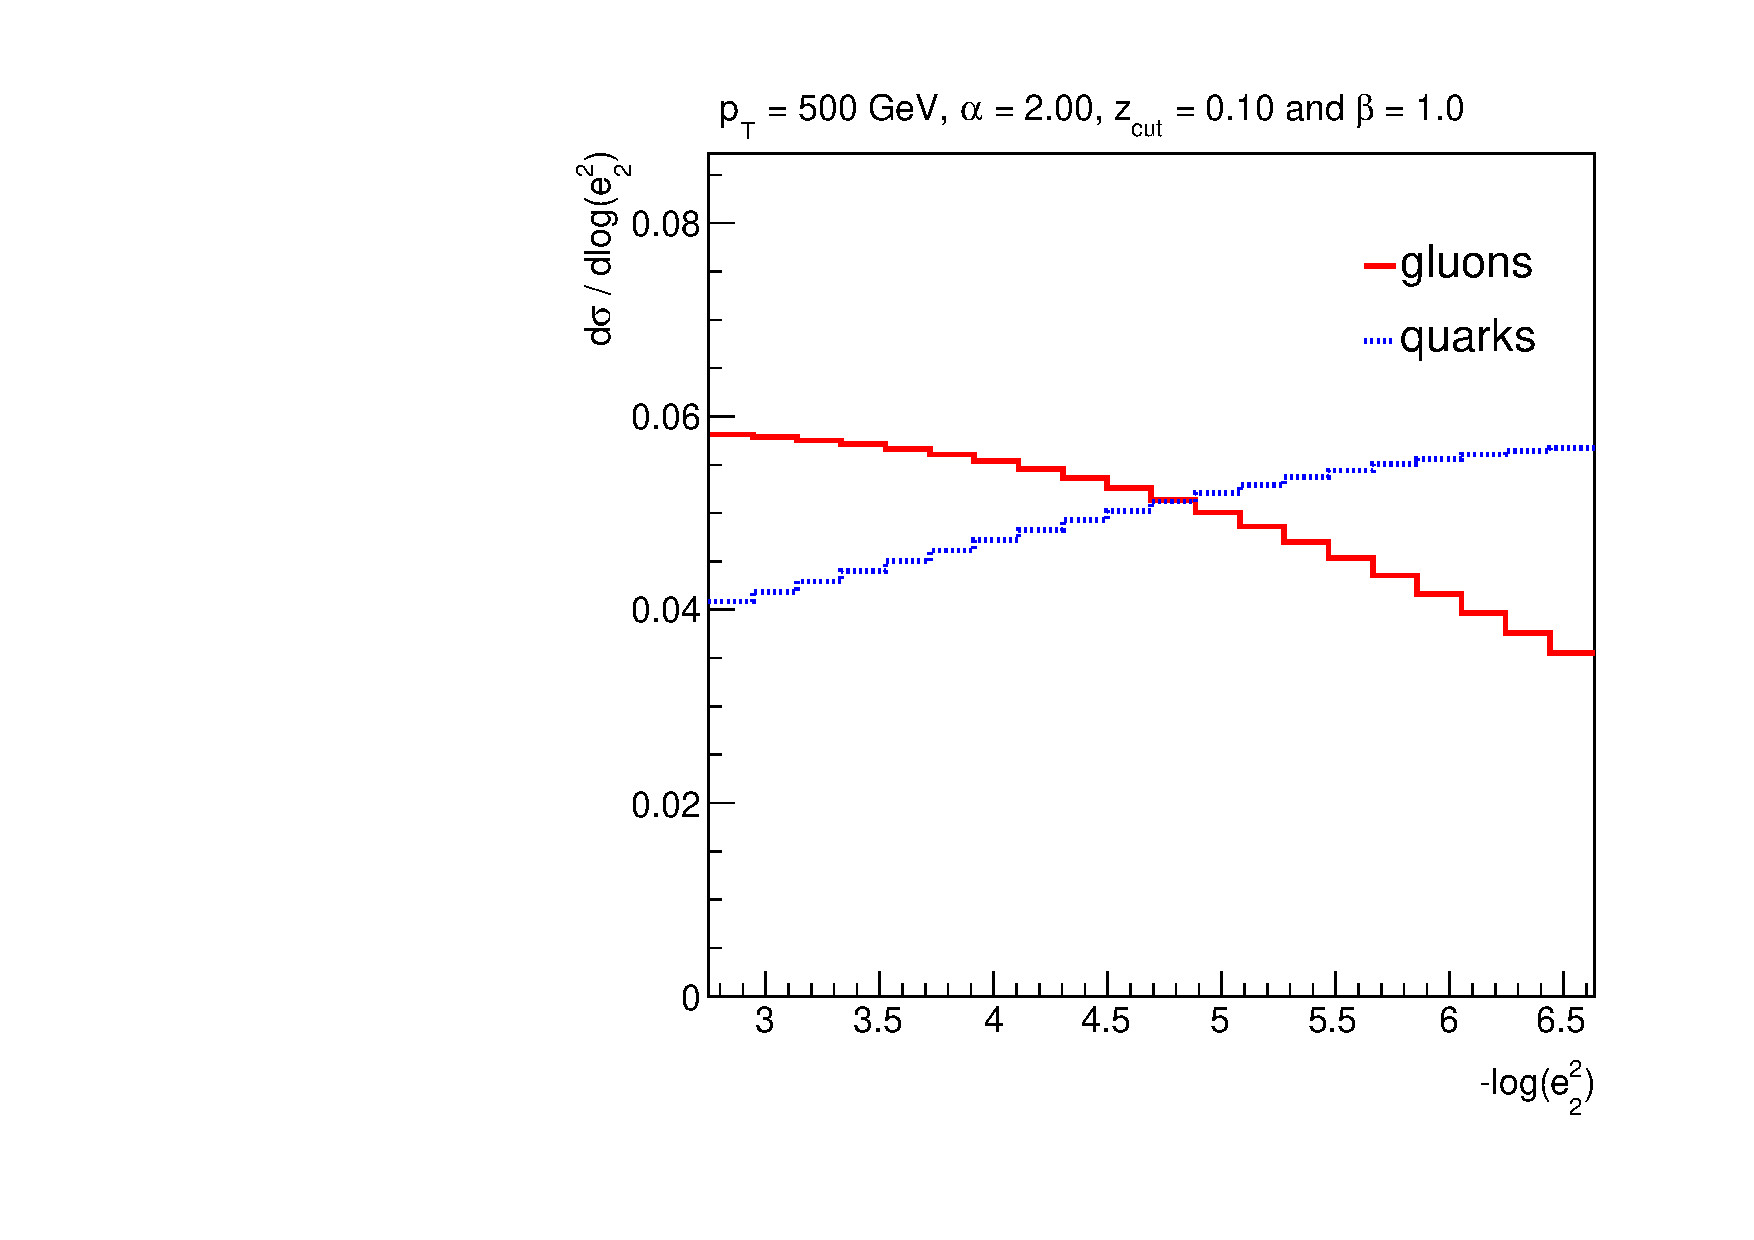
\includegraphics[width = 0.49\columnwidth]{figures/PDFs_alpha_20zcut1_beta_1023451324.pdf}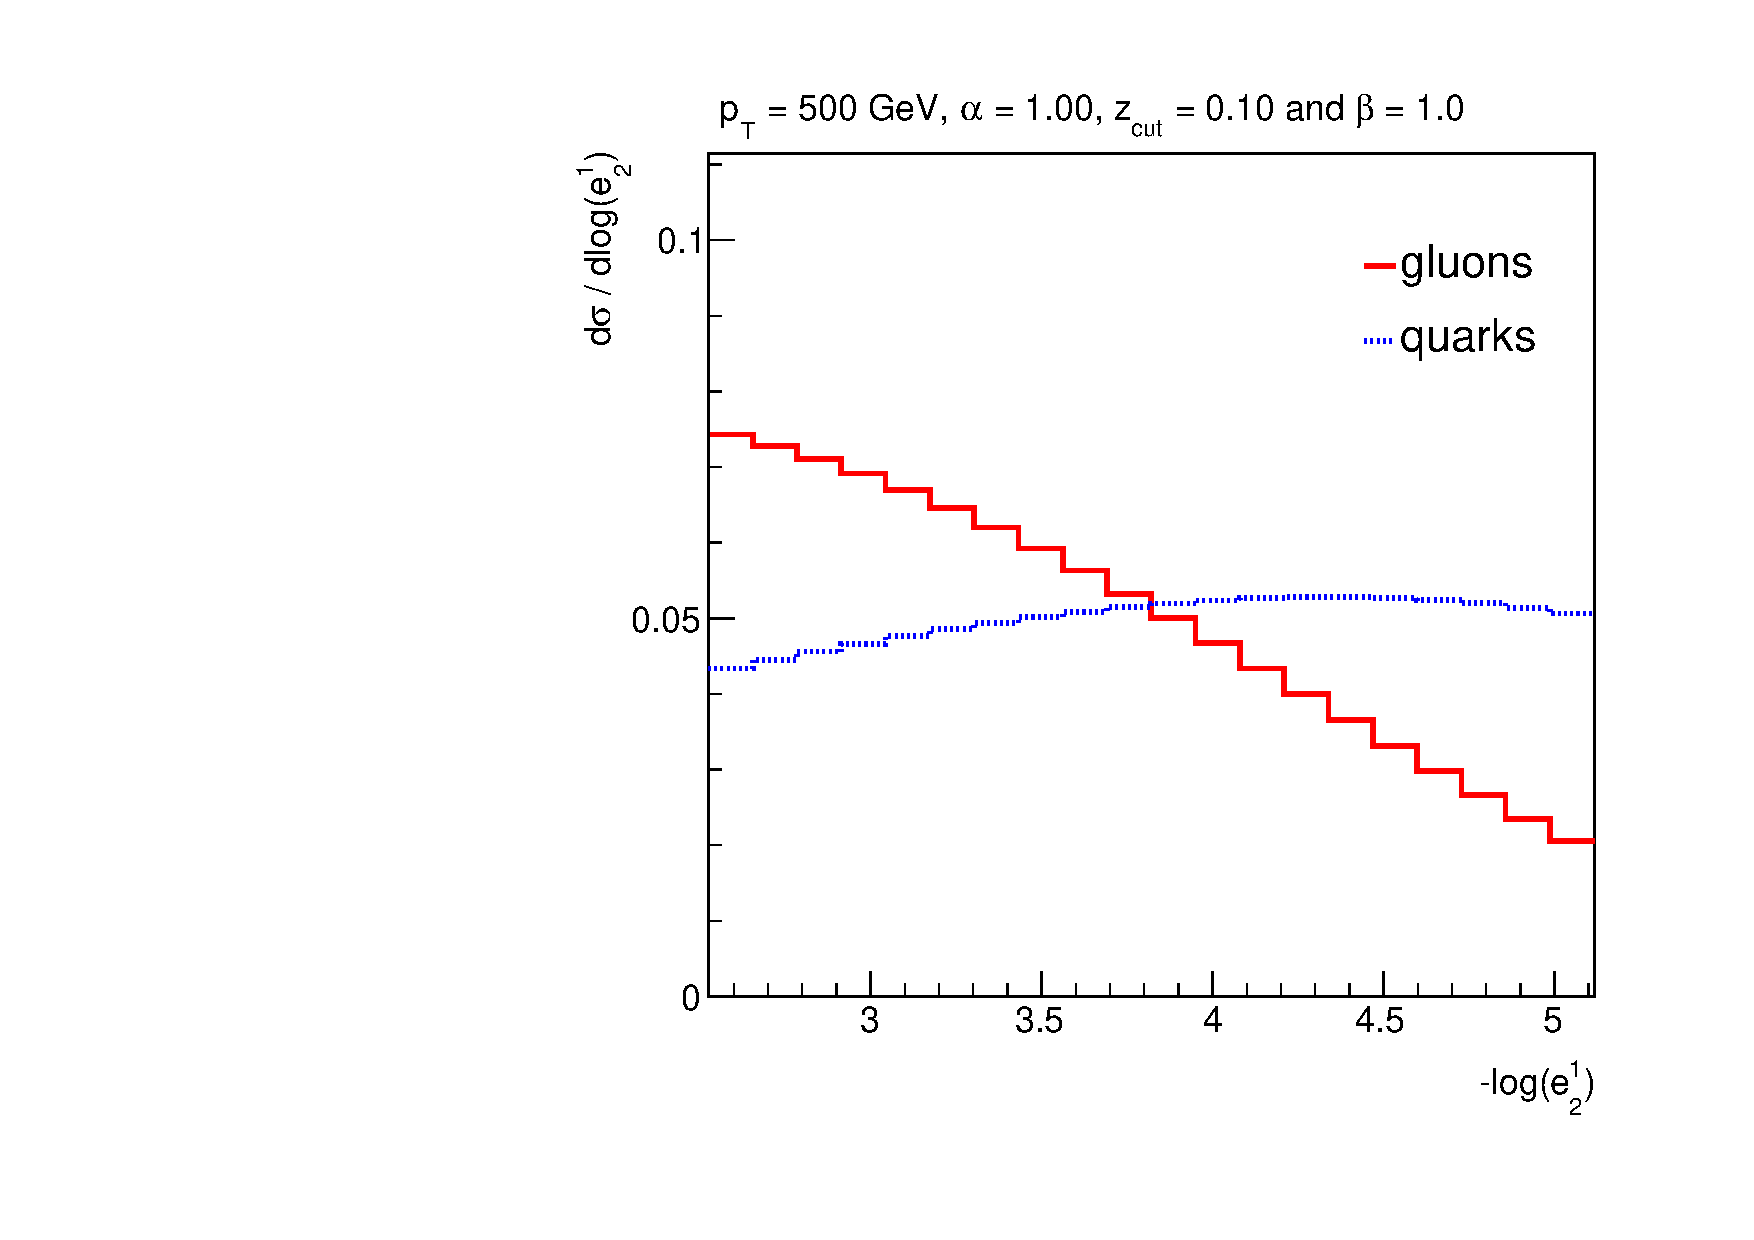
\includegraphics[width = 0.49\columnwidth]{figures/PDFs_alpha_10zcut1_beta_1023451324.pdf}\\
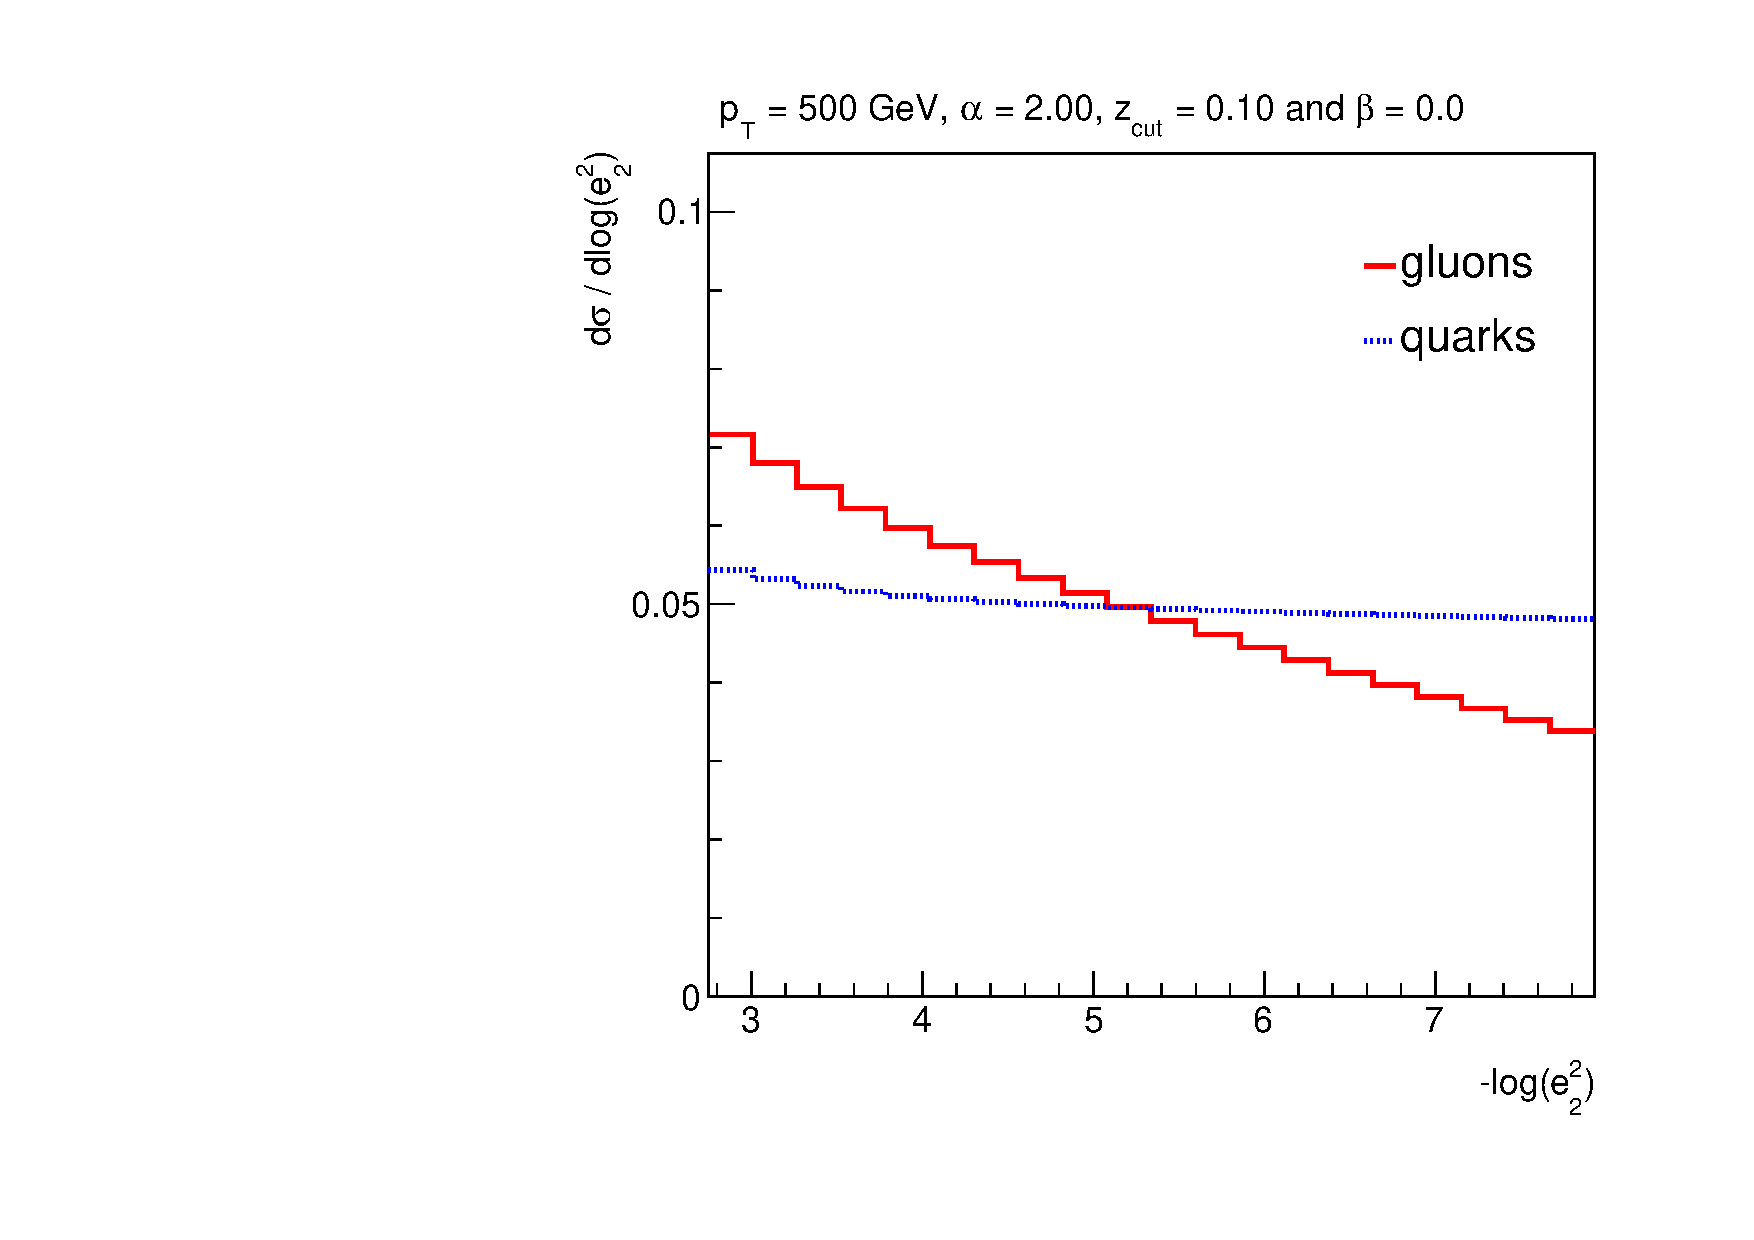
\includegraphics[width = 0.49\columnwidth]{figures/PDFs_alpha_20zcut1_beta_023451324.pdf}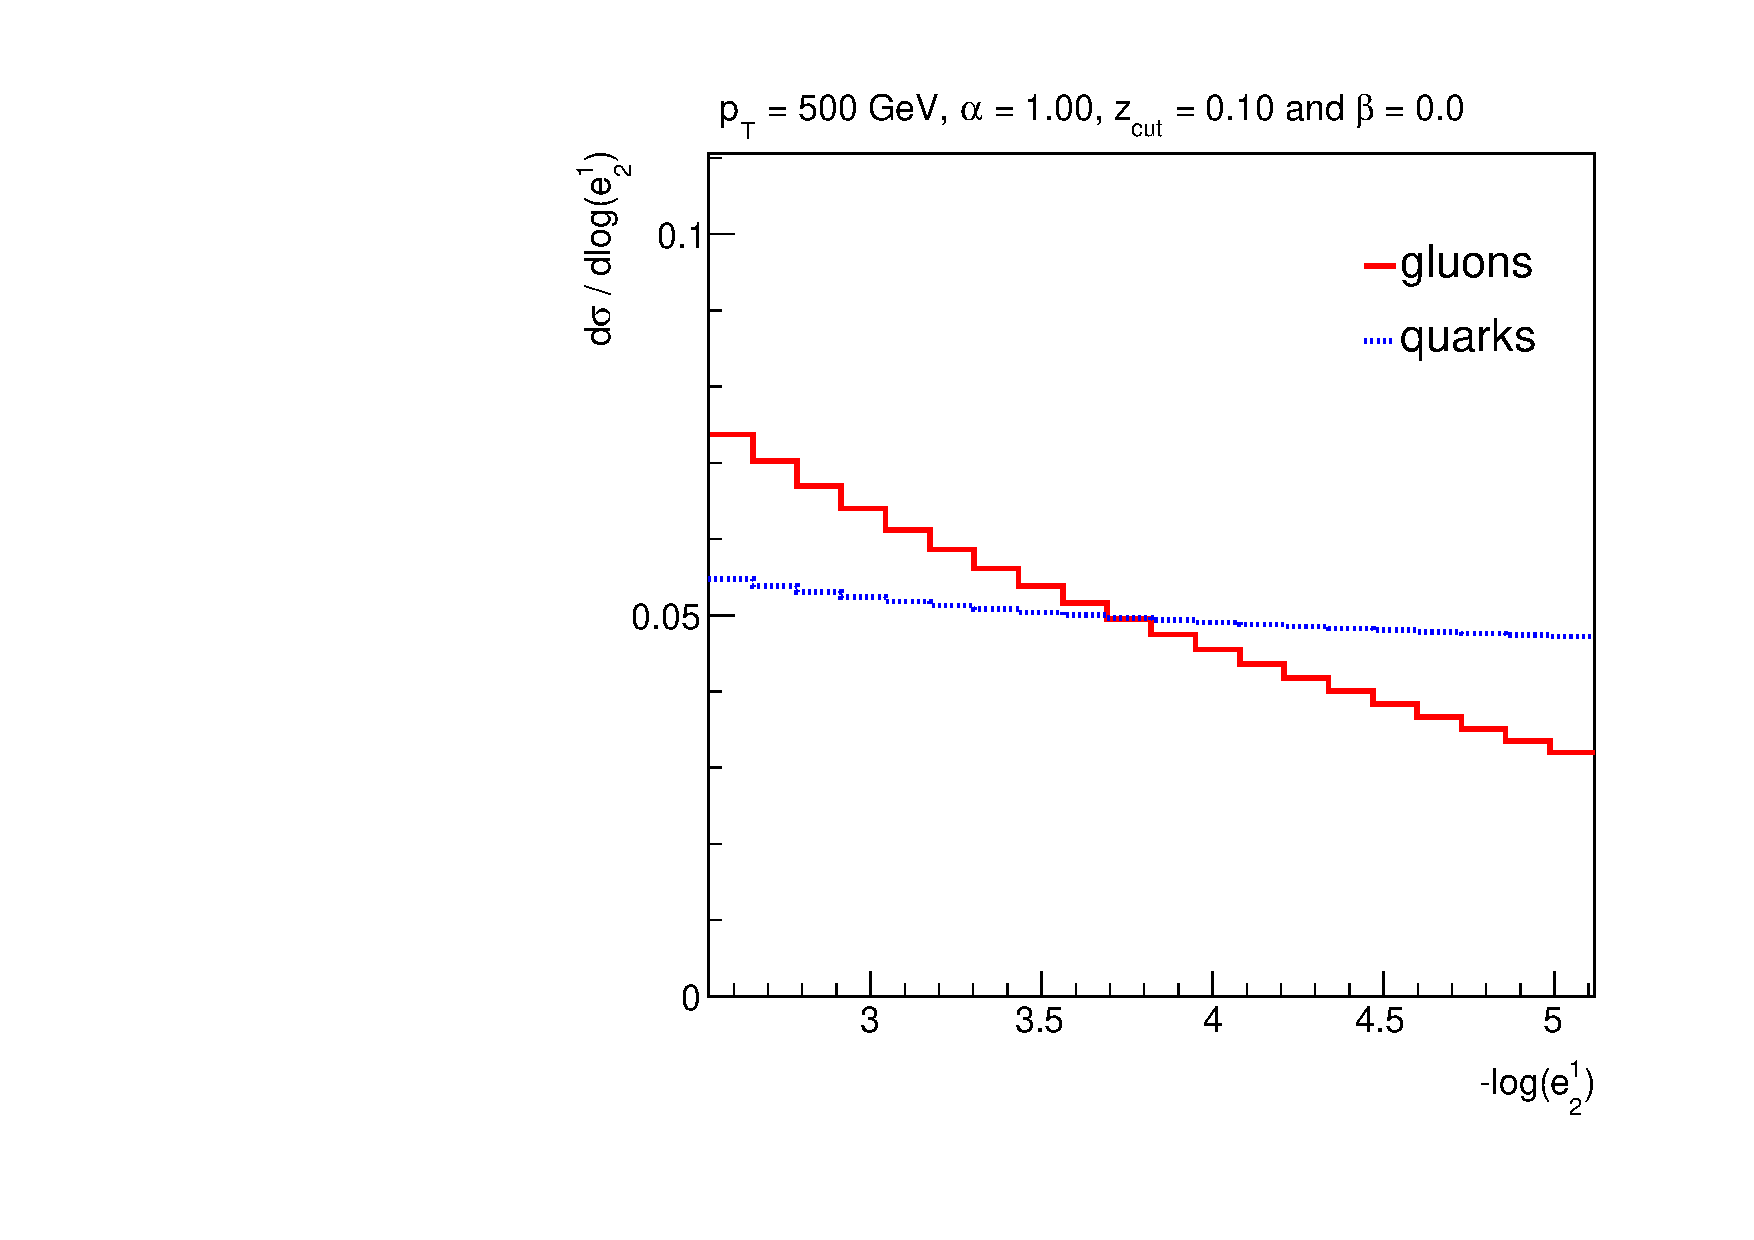
\includegraphics[width = 0.49\columnwidth]{figures/PDFs_alpha_10zcut1_beta_023451324.pdf}
\end{center}

%\jdt{We should decide whether or not it is important to have the plot in the same direction as \Fig{fig:shape_function}.}
%BPN: it would be nice if they all went in the same direction, but all of our plots are at least consistent (e.g. Fig. 5-7 and the ones here).  So hopefully it is okay to leave them as is.

\caption{The quark and gluon templates, computed at NLL~\cite{Marzani:2017mva,Marzani:2017kqd} for $\alpha=2$ (left column) and 
  $\alpha=1$ (right column), with grooming parameters $\zcut = 0.1$ and $\beta = 1$ (top row) and $\beta = 0$ (bottom row).  Note that larger masses are on the left so that the NP regime is on the
  right and the fixed-order regime is on the left.}
\label{fig:templates}
\end{figure}

From these NLL distributions, pseudo-data are then generated from the binned analytic probability distribution $t(\alpha_s,f_g)$.
%
These distributions are a superposition of the quark and gluon distributions and depend only on $\alpha_s$ and $f_g$.
%
Each pseudo-dataset has $n$ events and its binned representation is denoted by $h(\alpha_s,f_g,n)$.
%
For a given pseudo-dataset, the fitted values of $\alpha_s$ and $f_g$ are determined from a $\chi^2$-like fit:
%
\begin{align}
\label{eq:chi2fit}
\alpha_s,f_g=\text{argmin} \sum_i \frac{\left(h_i(\alpha_s,f_g,n)-t_i(\alpha_s,f_g)\right)^2}{\sigma(h_i(\alpha_s,f_g,n))^2},
\end{align}
%
where $t_i, h_i$ are the bin content of histograms $t$ and $h$, and $\sigma(h_i)$ is the statistical uncertainty in bin $i$ of histogram $h$.
%
In practice, there would also be systematic uncertainties (see \Sec{sec:resolution}), but the purpose of this study is to simply illustrate the sensitivity to $\alpha_s$ and $f_g$ for a given number of events.


	
\begin{figure}[t]
\begin{center}
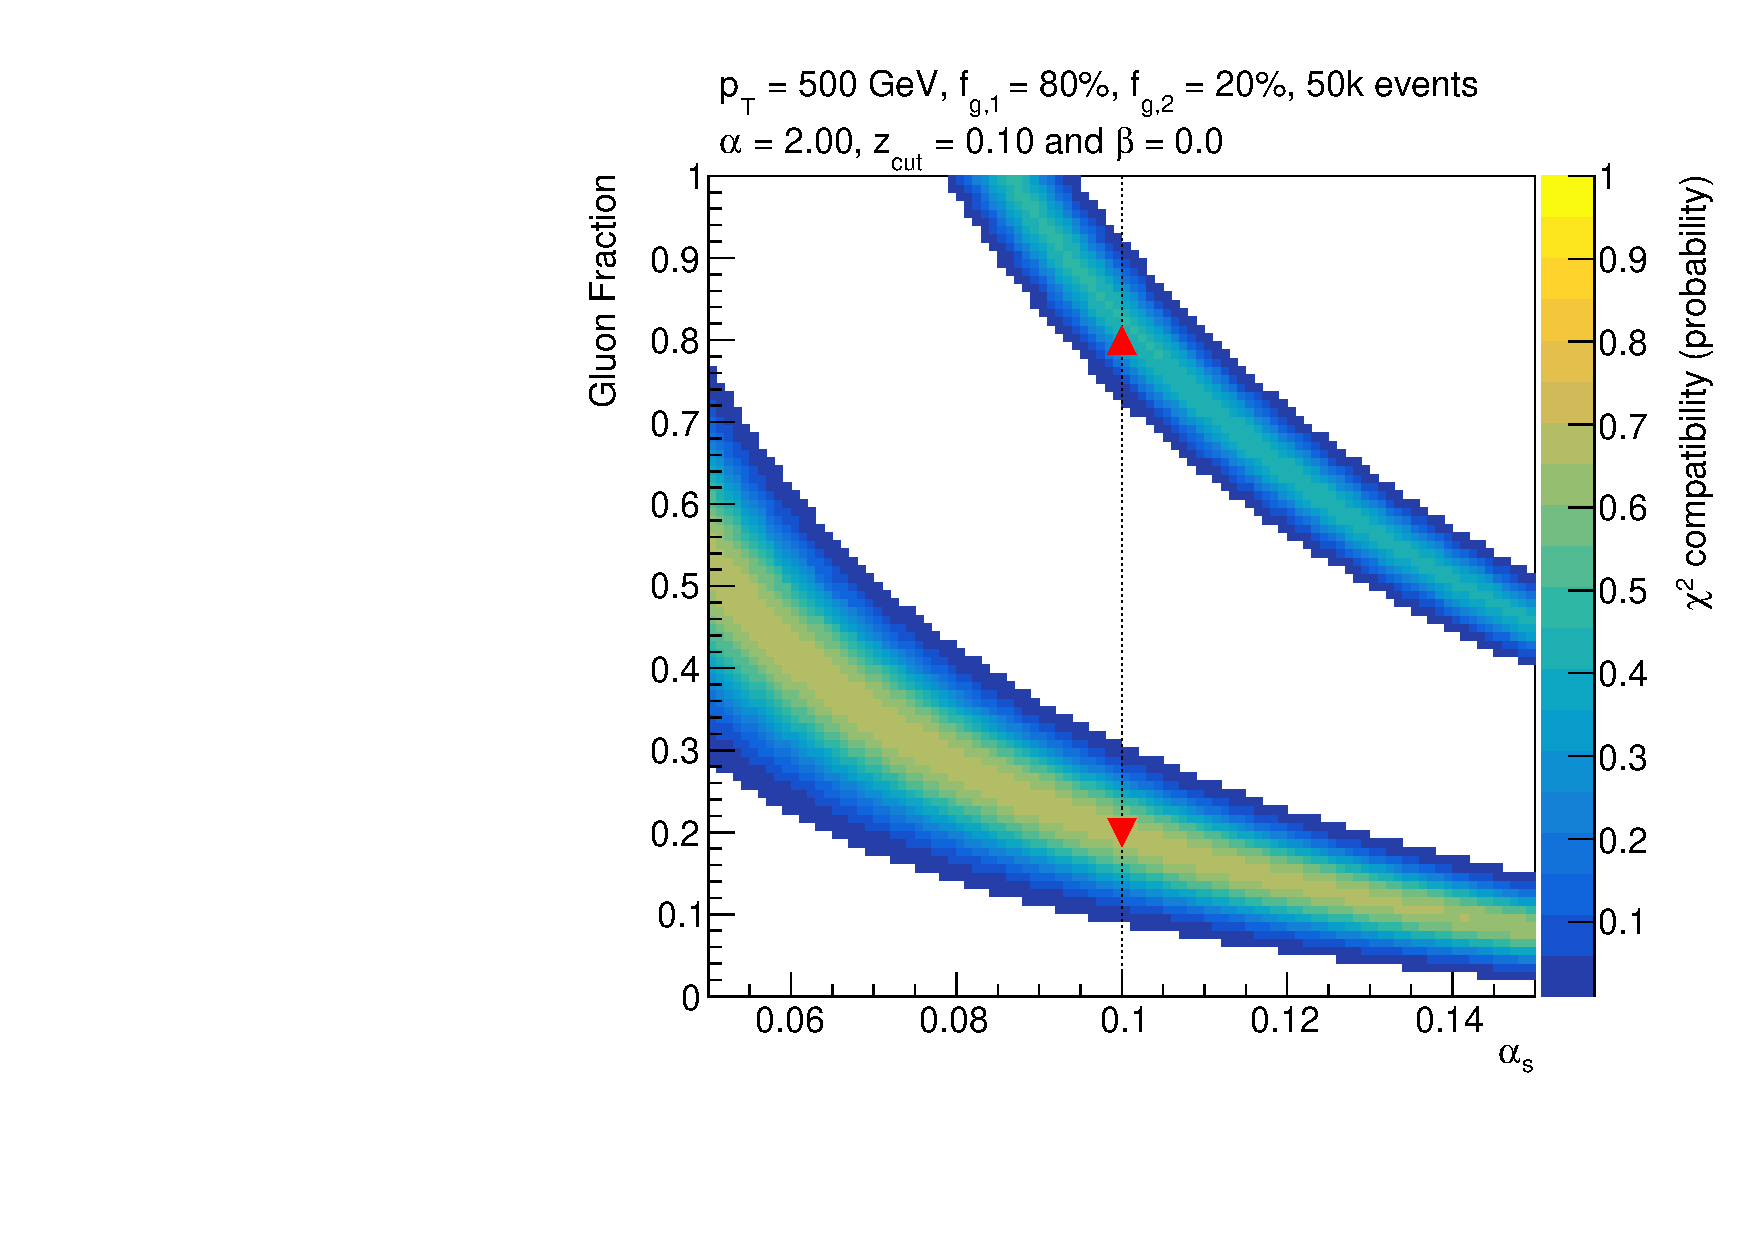
\includegraphics[width = 0.49\columnwidth]{figures/banana_alpha_20beta_0_zcut_123451324.pdf}
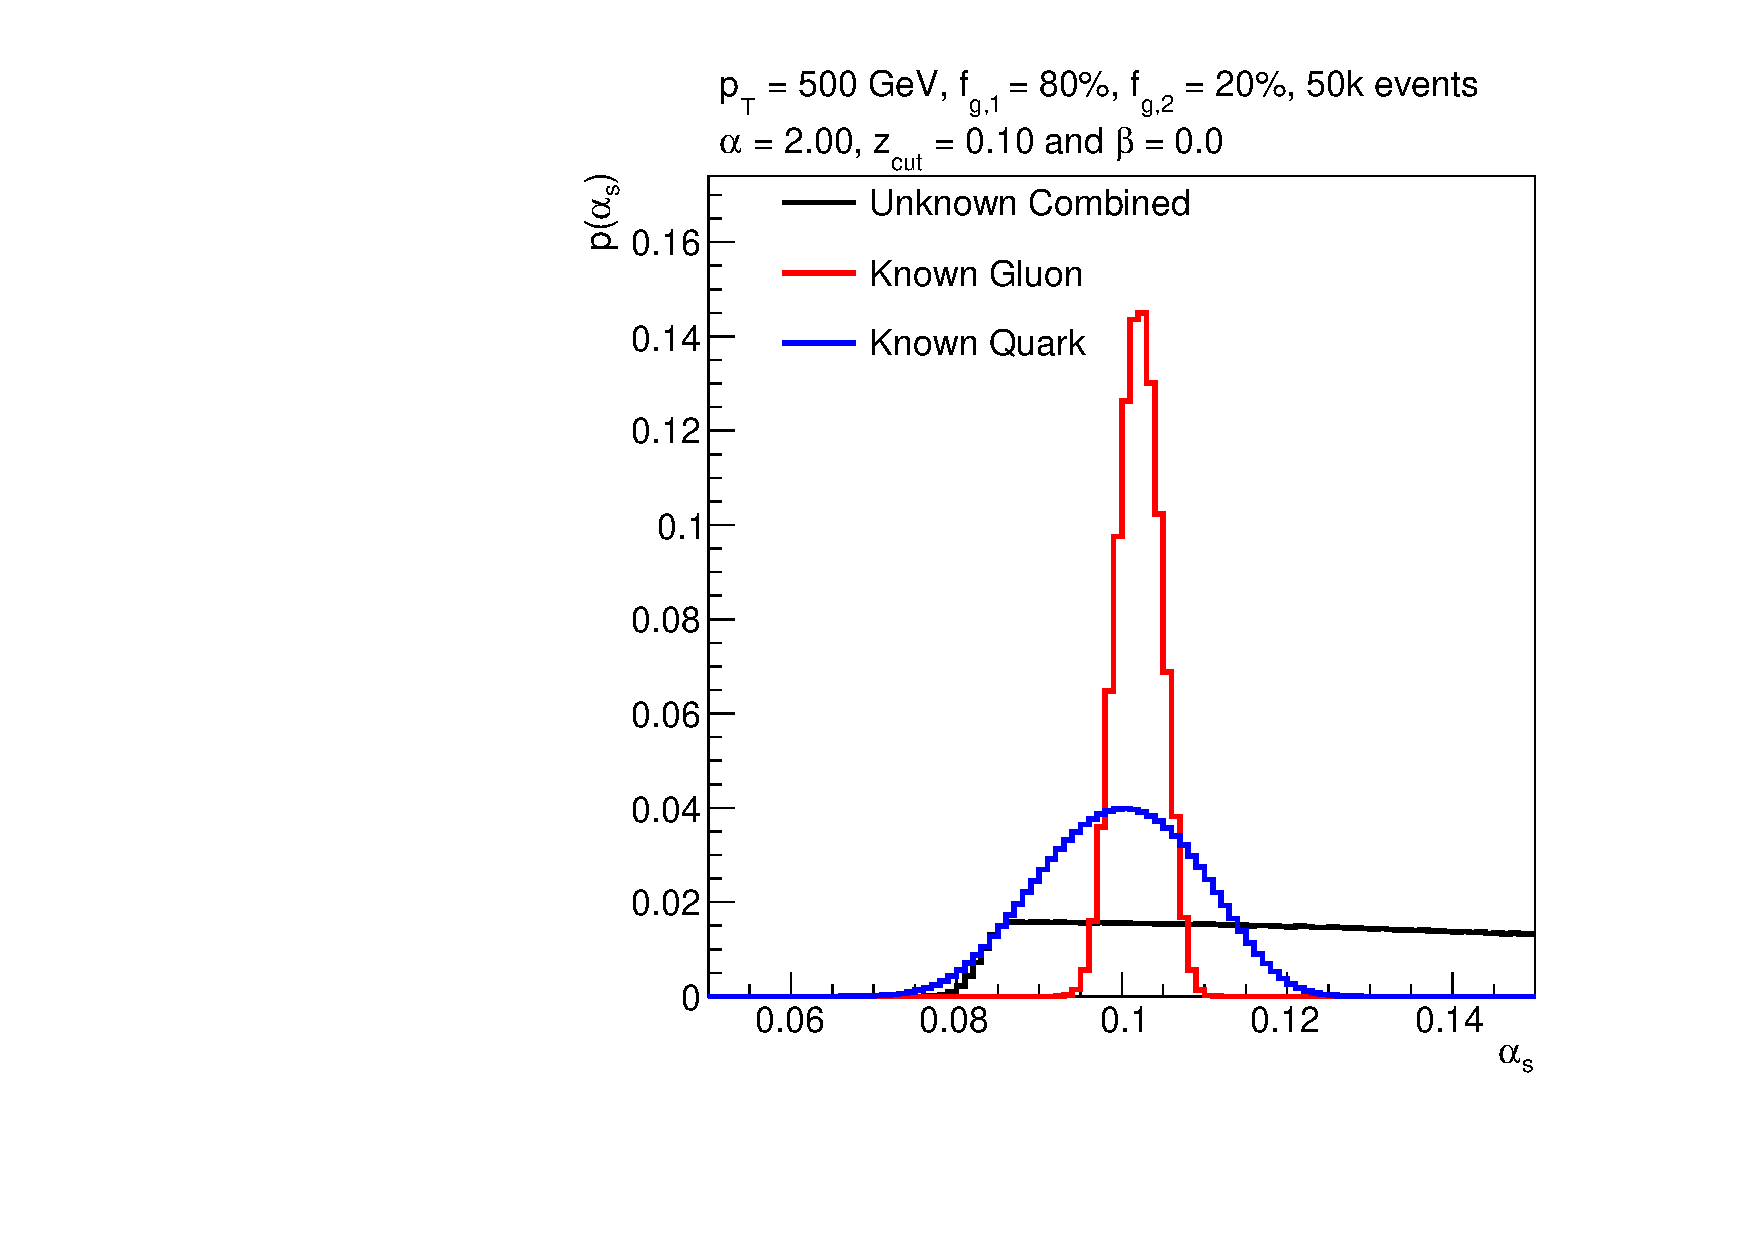
\includegraphics[width = 0.49\columnwidth]{figures/palpha_alpha_20beta_0_zcut_123451324.pdf}
\end{center}
\caption{Left: the probability of the minimized $\chi^2$ (assuming $n_\text{bins}-1$ degrees of freedom) from \Eq{eq:chi2fit} as a
  function of $f_g$ and $\alpha_s$ for one sample with 80\% gluons and another sample with 80\% quarks.  The true value of $\alpha_s$ is 0.1, as indicated by triangle markers.  Right: The right plot marginalized over $f_g$ and normalized to unity.  The three lines correspond to the fit performed on a pure sample of quarks, a pure sample of gluons, or a mixed sample of ($f_g\in\{0.2,0.8\}$) where the fractions are not known a priori.  This is the result from one pseudo-experiment with 100k events.}
\label{fig:alpha2fit}
\end{figure}



%
An example fit is demonstrated in \Fig{fig:alpha2fit} for the case of $\alpha=2$ and $\beta = 0$.
%
The left plot of \Fig{fig:alpha2fit} shows the $\chi^2$ from \Eq{eq:chi2fit} for two samples, one with 20\% gluons and one with 80\% gluons.
%
The true value is taken to be $\alpha_s=0.1$, and as expected, the $\chi^2$ probability is high for $f_g=0.2$ and $f_g=0.8$.%
\footnote{It is not necessarily peaked at this value because this is the result of one pseudo-experiment.  Averaging over many pseudo-experiments results in peaks at $f_g=0.2$ and $0.8$.}
%
The banana shapes of the curves are a consequence of the degeneracy due to Casimir scaling discussed in \Sec{sec:casimir}.
%
From one sample alone, there is essentially no ability to distinguish between a larger $\alpha_s$ and a smaller $f_g$; the only constraint comes from the fact $0\leq f_g\leq 1$ which results in a crude bound on $\alpha_s$.
%
This is shown in the right plot of \Fig{fig:alpha2fit} where the distribution is marginalized over $f_g$ and normalized to unity.
%
One can view this as the posterior probability of the fitted $\alpha_s$: the peak is the fitted value of $\alpha_s$ and the width is the uncertainty.
%
When $f_g$ is known, the uncertainty in $\alpha_s$ is significantly reduced; this is illustrated with pure quark and gluon samples.
%
Due to the larger color factor, the measurement with pure gluon jets is more sensitive to $\alpha_s$ than the fit using pure quark jets, as anticipated in \Sec{sec:analytic}.
%
Using both the $f_g=0.2$ and $f_g=0.8$ samples to fit for $\alpha_s$, one can extract a $\sim 30\%$ measurement of $\alpha_s$, but there is no clear peak at the correct value of $\alpha_s$ due to the Casimir degeneracy.  

%   \gs{The legend on the
%    right plot is potentially misleading, I'd say ``known $f_g=20\%$''
%    and ``known $f_g=80\%$''. If easily doable, it might also be good
%    to have the extracted alphas (central value+uncertainty).} \gs{Why
%    has the left plot changed that much compared to the previous
%    version?} 

\begin{figure}[t]
\begin{center}
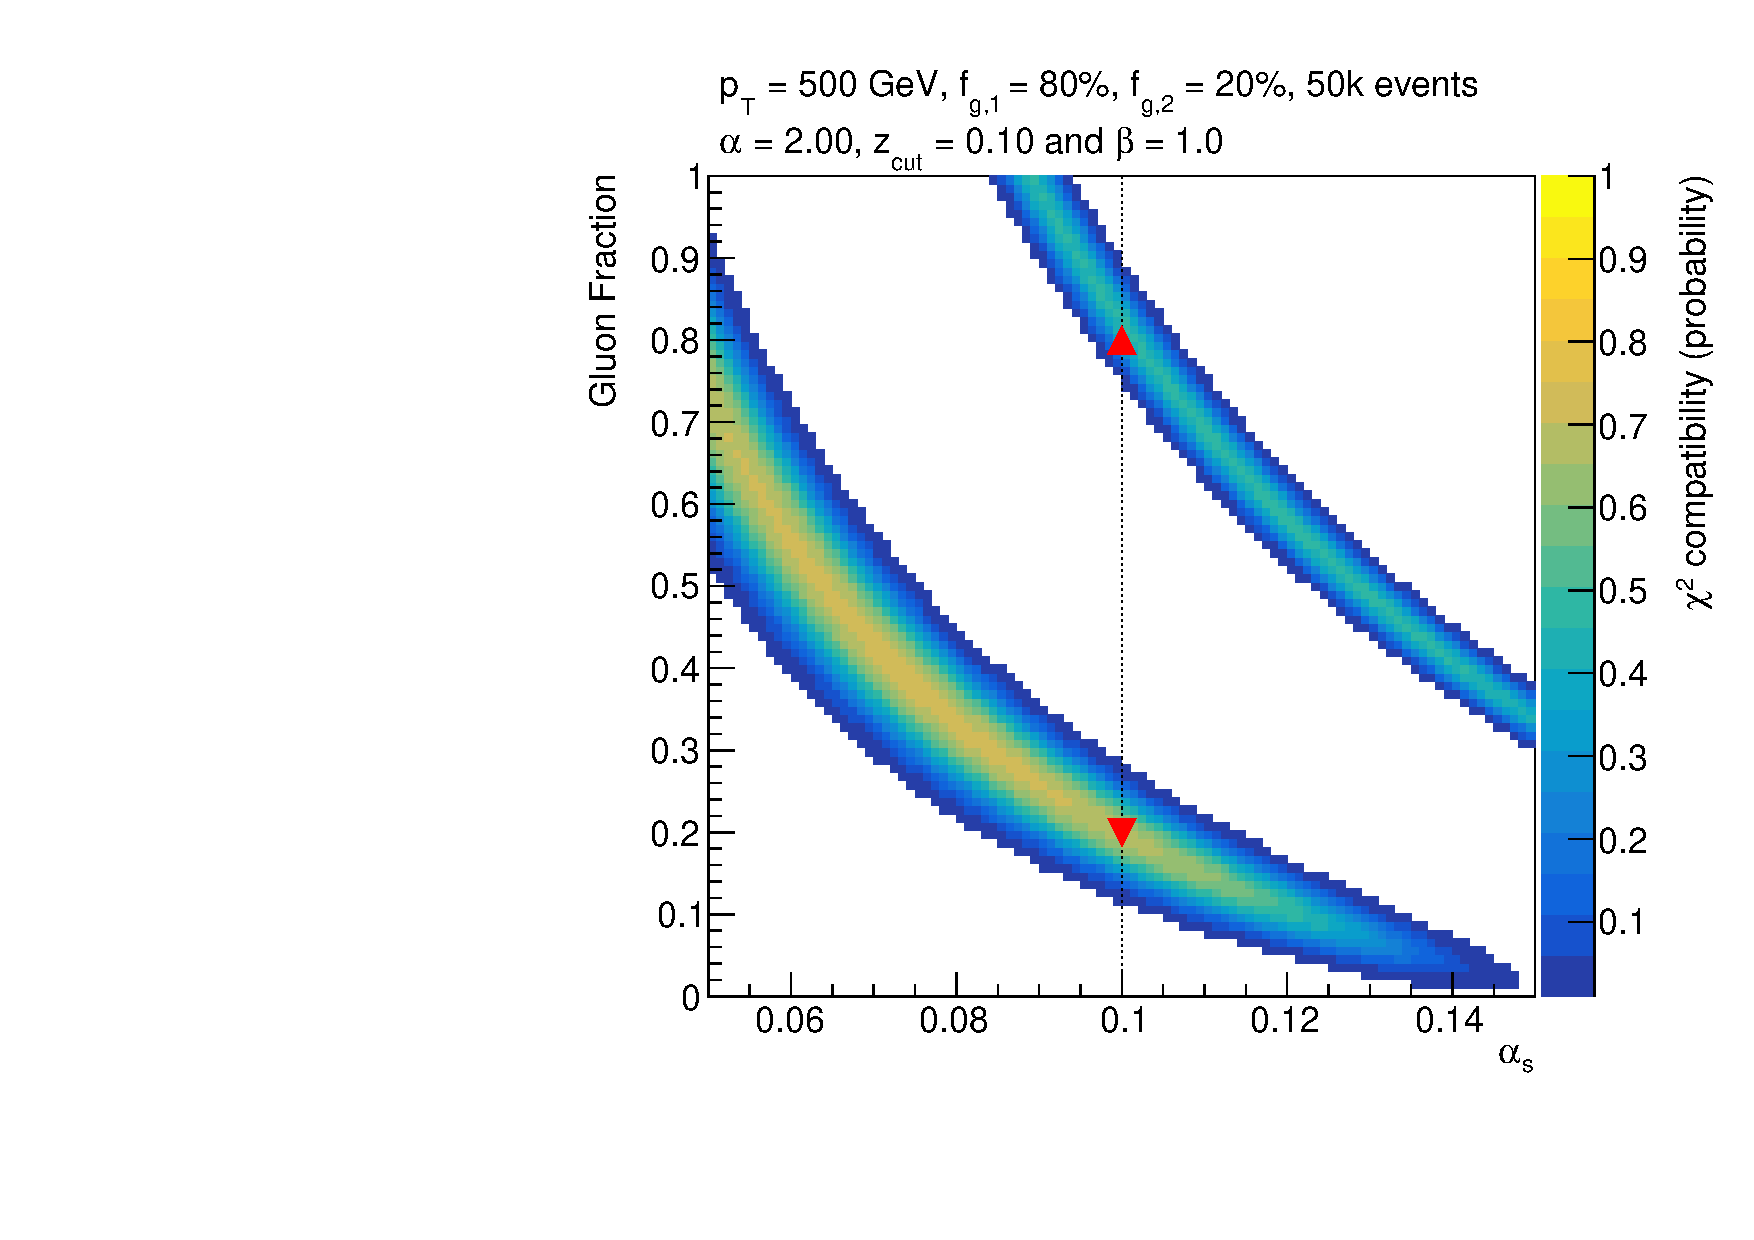
\includegraphics[width = 0.32\columnwidth]{figures/banana_alpha_20beta_10_zcut_123451324.pdf}
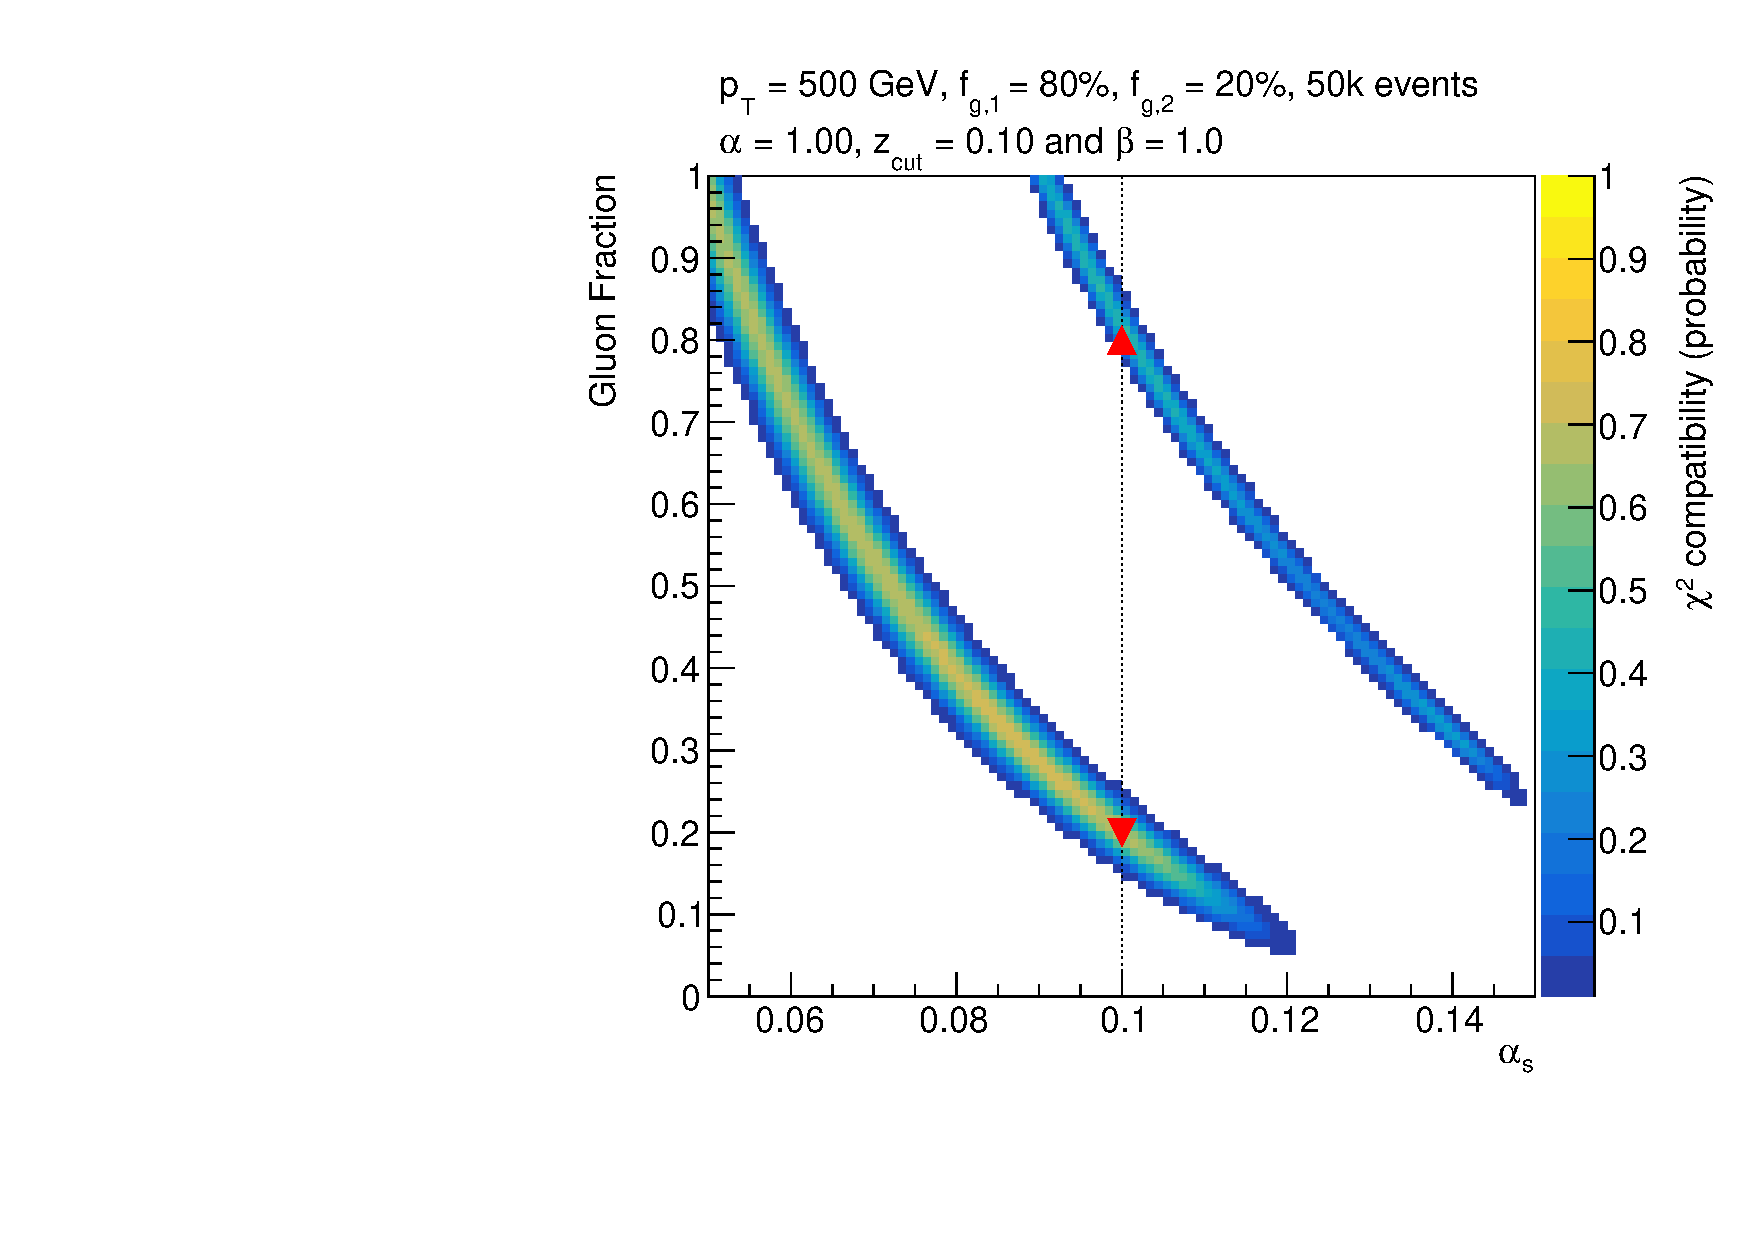
\includegraphics[width = 0.32\columnwidth]{figures/banana_alpha_10beta_10_zcut_123451324.pdf}
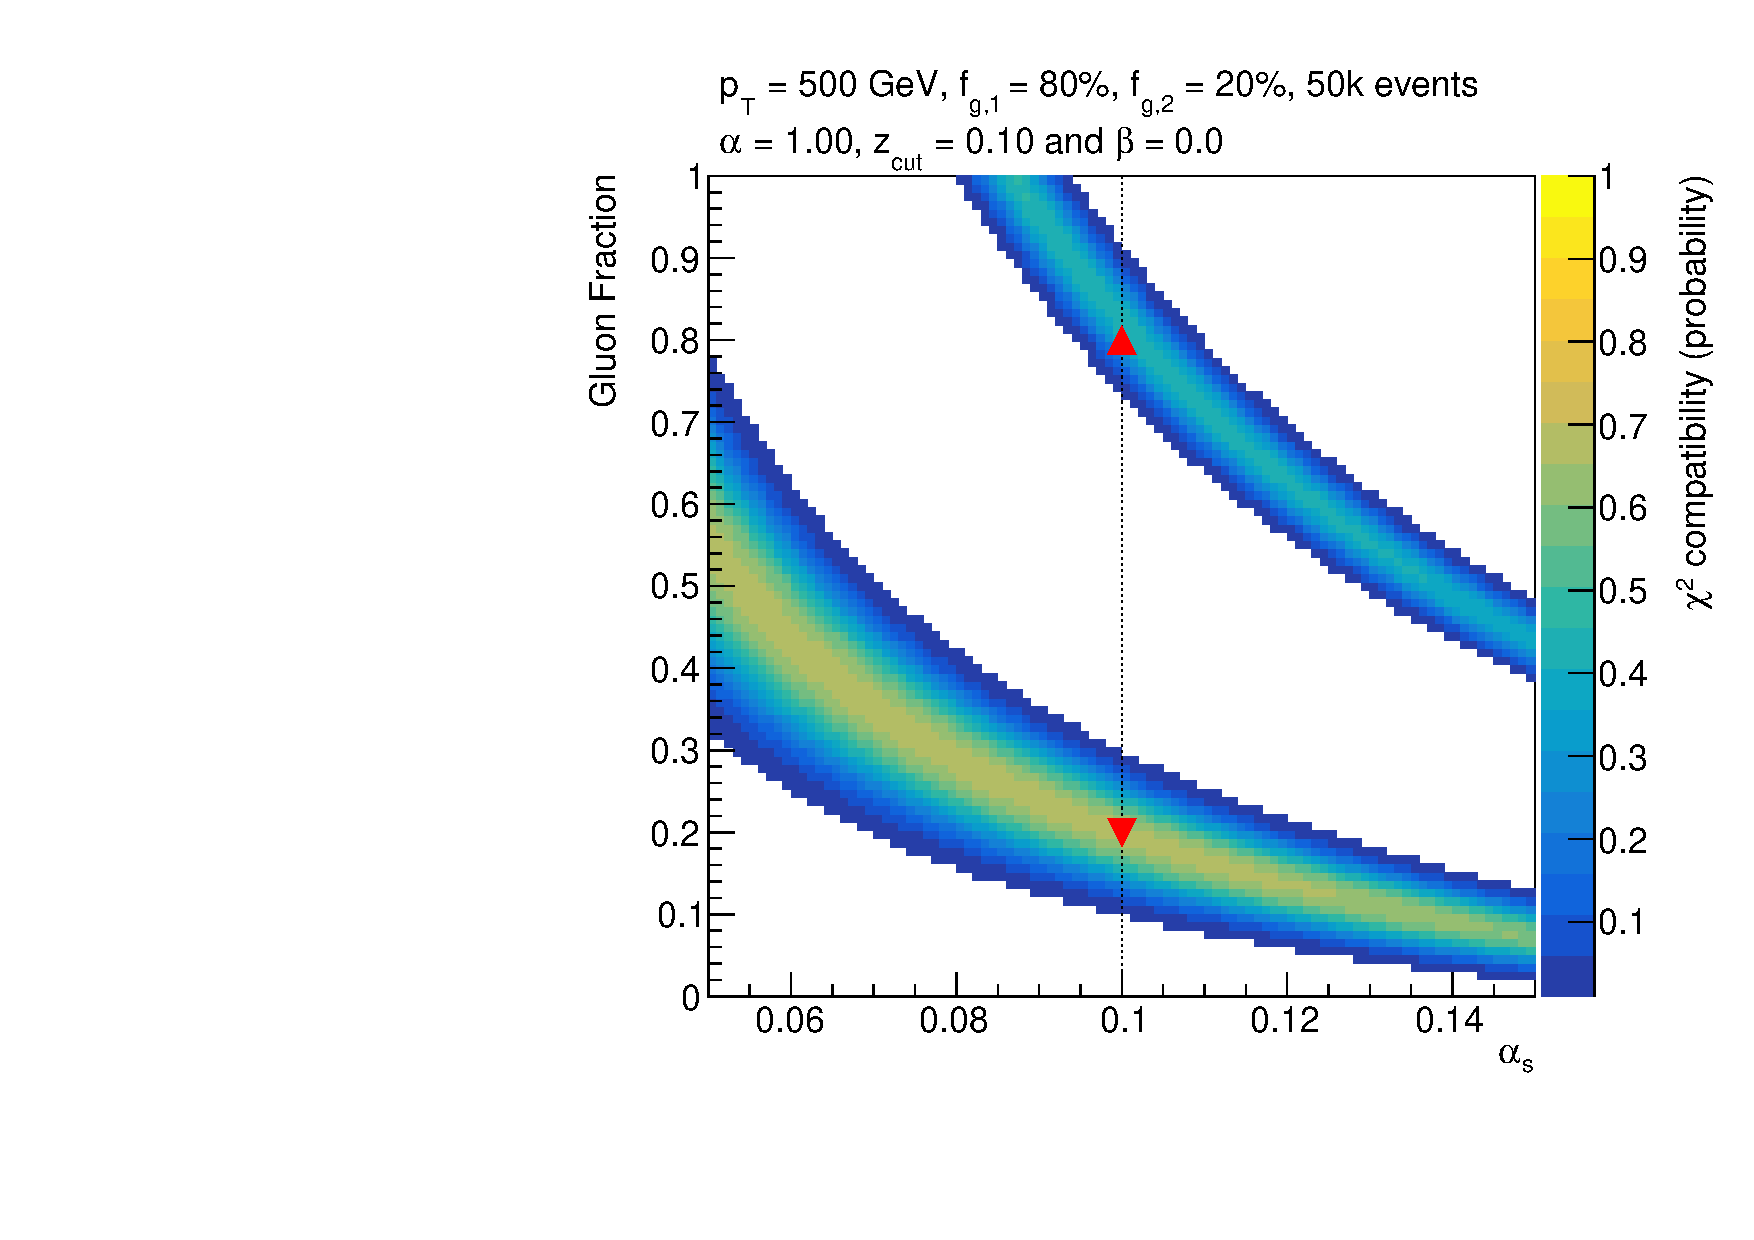
\includegraphics[width = 0.32\columnwidth]{figures/banana_alpha_10beta_0_zcut_123451324.pdf}
\end{center}
\caption{The same as the left plot of \Fig{fig:alpha2fit}, but for the remaining three observables from \Fig{fig:templates}.}
\label{fig:morebananas}
\end{figure}


One way to improve the situation is to combine multiple $\alpha$, $\beta$, and $z_\text{cut}$ values (only $\alpha$ and $\beta$ are varied here).
%
Figure~\ref{fig:morebananas} shows the $f_g,\alpha_s$ fit for all of the $\alpha,\beta$ values from \Fig{fig:templates} that were not shown in \Fig{fig:alpha2fit}.
%
As in \Fig{fig:alpha2fit}, there are two banana-shaped regions that correspond to the $f_g=20\%$ and $f_g=80\%$ samples.
%
The tilt of the bananas is slightly different than the $\alpha=2$, $\beta=0$ case and so there is a possibility to gain from combining the information in the observables.
%
In practice, a challenge with a multi-observable extraction strategy is the need to understand correlations between observables.
%
At the moment, joint distributions of two-point correlators are only known to NLL accuracy without grooming~\cite{Larkoski:2014pca}.

\begin{figure}[t]
\begin{center}
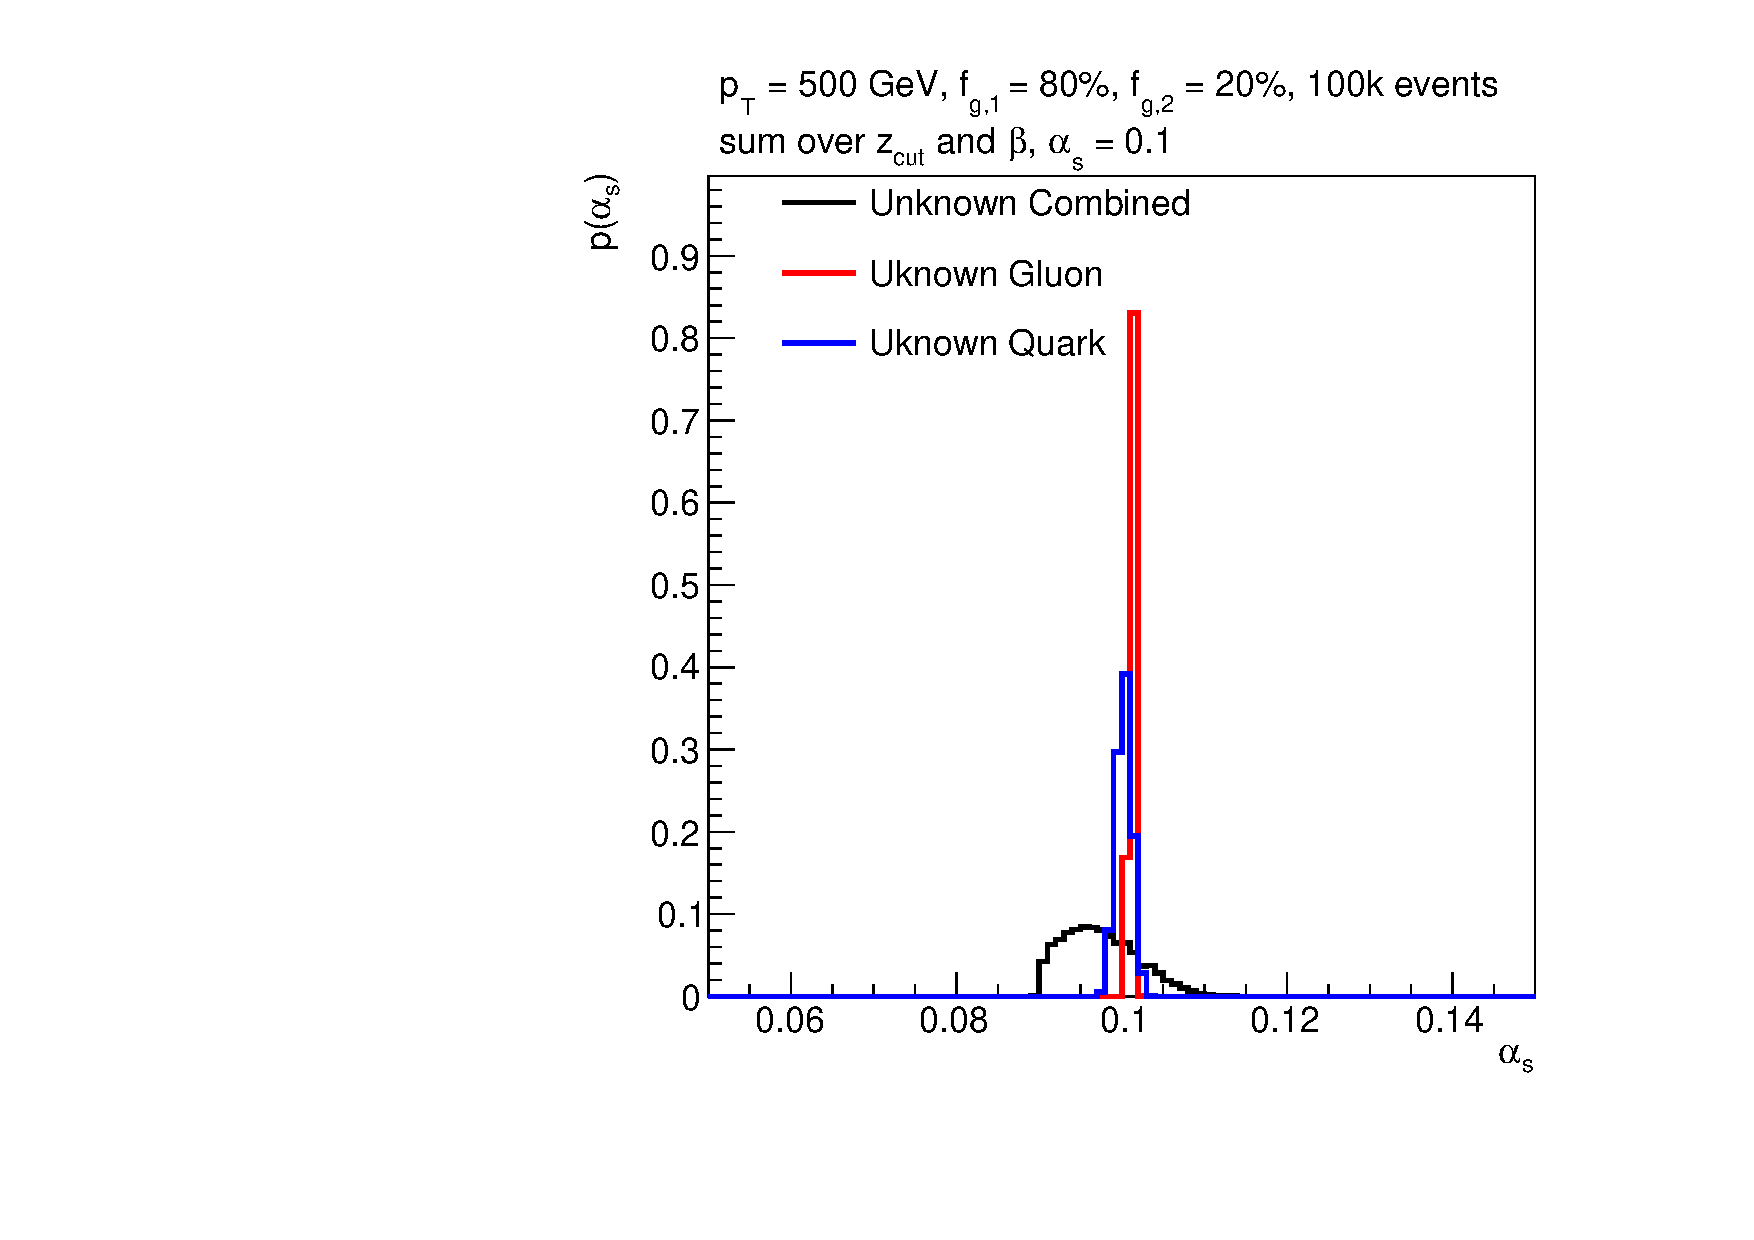
\includegraphics[width = 0.49\columnwidth]{figures/combination23451324.pdf}
%combination23451324
\end{center}
\caption{Marginalizing the $f_g,\alpha_s$ fit over the gluon fraction for a fit that combines the four observables from \Fig{fig:templates}.  The unknown combined mixture uses two samples with $f_g=20\%$ and $f_g=80\%$.}
\label{fig:combo}
\end{figure}

With that caveat in mind, Figure~\ref{fig:combo} shows the result of a combined fit assuming that all four distributions are statistically (and systematically) independent
%
This is a rather strong assumption that is unlikely to be even approximately true in practice.
%
However, the benefit of having different tilts in the $f_g,\alpha_s$ plane is clearly shown and would be a generic feature of a multi-observable fit, even if the size of the gain is not as significant as shown here.
%
It is important to emphasize that the black curve in \Fig{fig:combo} assumes no prior knowledge of the gluon fraction of the event samples.
%
The fit can of course be improved by using some knowledge of the gluon fractions from the hard scattering process convolved with PDFs, as discussed in \Sec{subsec:norm}.

%\gs{Varying $z_{\text{cut}}$ and $\beta$ would also change the slope
%  (maybe not in the 2d maps), so we could add something saying that it
%  would be interesting to study those variations as well.} 

\subsection{Estimate of Experimental Resolution}
\label{sec:resolution}

To keep pace with precise theory predictions, the experimental resolution must be well-understood in order to ensure both precision and accuracy of jet substructure measurements.
%
To estimate the impact of detector resolution on $\alpha_s$ fit illustrated in \Sec{sec:templates}, a fast simulation from \textsc{Delphes} 3.4.1~\cite{deFavereau:2013fsa} was studied using particle-level input from \pythia.210.
%
This setup uses a CMS-like detector with jets built from particle-flow objects.
%
There are generically two regimes for determining the experimental resolution.
%
At high mass, there are well-resolved hard prongs in the jet, so the resolution is set by the jet energy resolution of those ``sub-jets''.
%
At low mass, the groomed jet is defined by nearly collinear splittings at which point the angular resolution can dominate.


\begin{figure}[t]
\begin{center}
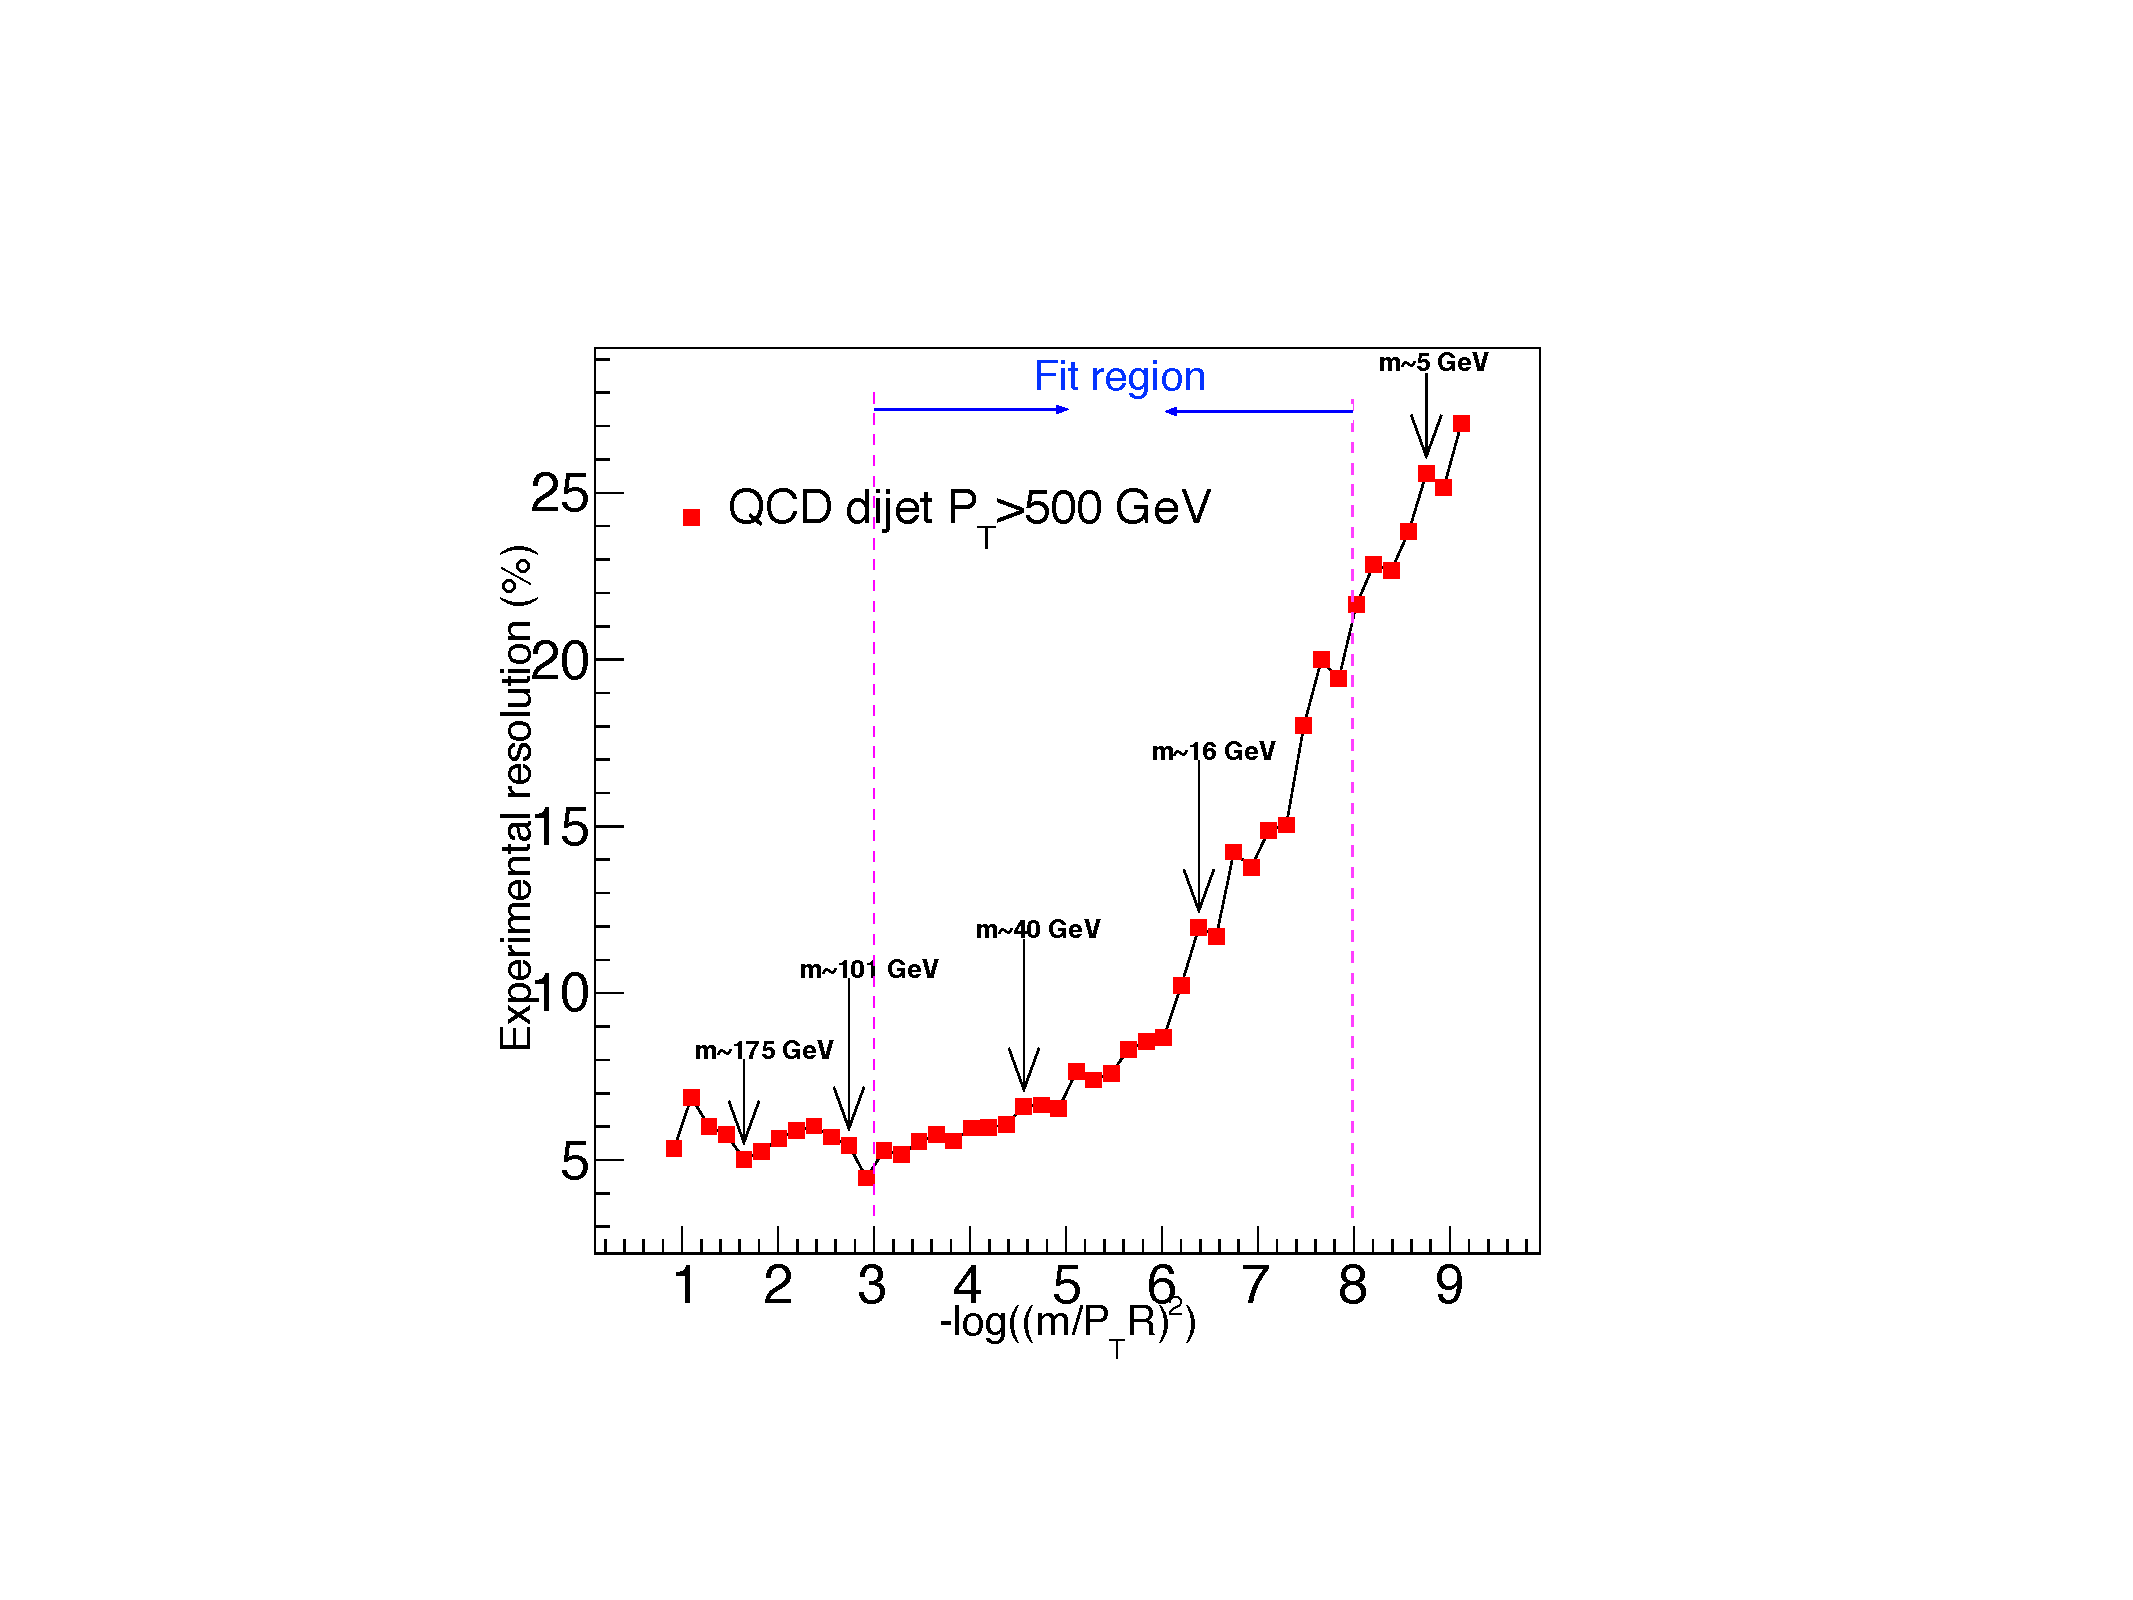
\includegraphics[width = 0.49\columnwidth]{figures/experimentaldemo/Resolution_plot_logrho_updated2.pdf}
\end{center}
\caption{The fractional $\ecf{2}{2}$ distribution determined from dijet events simulated with \pythia plus \textsc{Delphes}.  Arrows indicate the mass at given values of the two-point correlator.  The upper bound of the resummation regime is indicated by a dashed line.  Larger masses are to the left.}
\label{fig:resolution}
\end{figure}

\begin{figure}[t]
\begin{center}
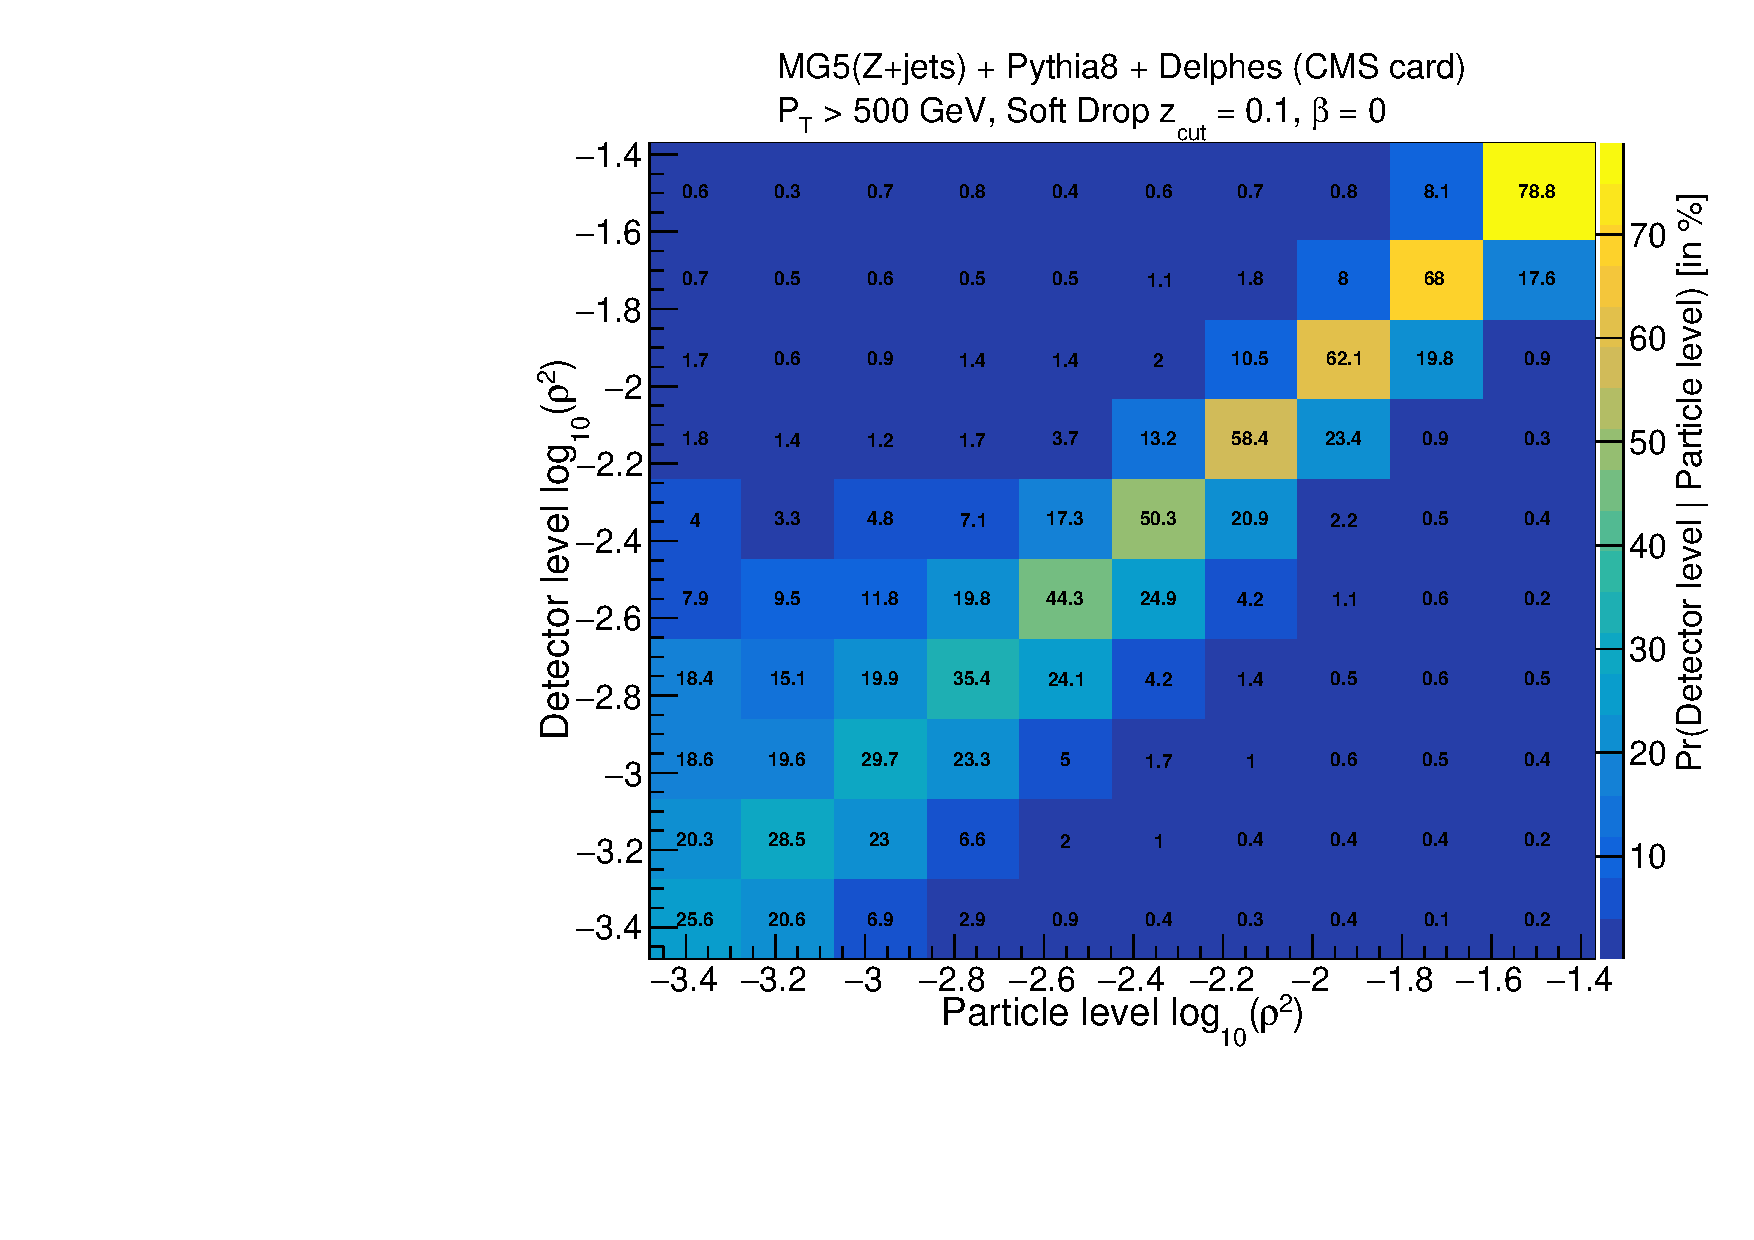
\includegraphics[width = 0.49\columnwidth]{figures/experimentaldemo/Rho_2D.pdf}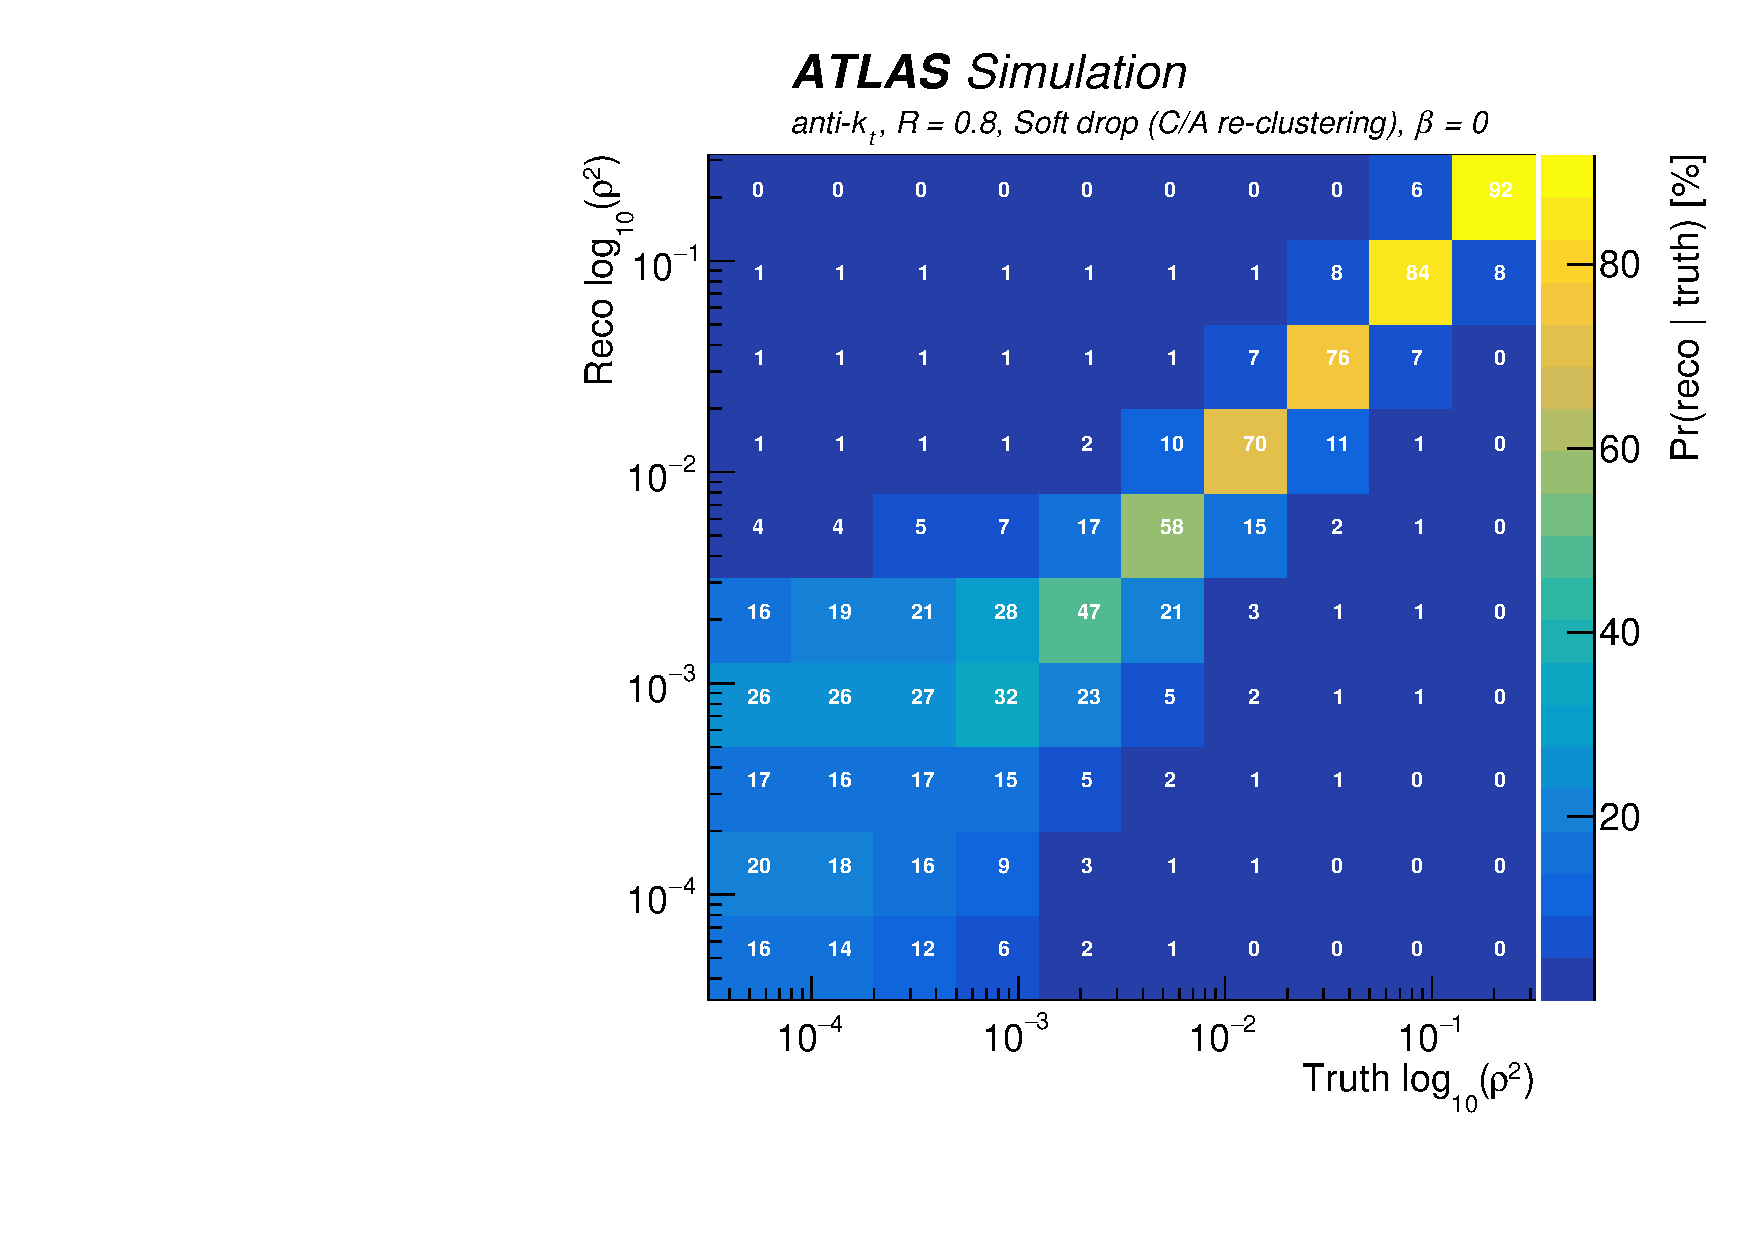
\includegraphics[width = 0.49\columnwidth]{figures/figaux_03a.pdf}
\end{center}
\caption{Left: The migration matrix between particle-level and detector-level using the Delphes simulation (left) and from the ATLAS measurement (right; reproduced from \Ref{Aaboud:2017qwh}).  Unlike previous plots, larger masses are on the right (shown this way to match the ATLAS result). }
\label{fig:expres}
\end{figure}

Figure~\ref{fig:resolution} shows the fractional $\ecf{2}{2}$ resolution estimated from \textsc{Delphes}.
%
The resolution is smallest at high mass due to the excellent energy resolution of the CMS-like detector.
%
The resolution at low mass is about 10\% near 15 GeV and reaches 30\% near the limit of $\mathcal{O}(\text{few GeV})$.
%
Encouragingly, the fits in \Sec{sec:templates} relied only on the regime where $\sim 10\%$ resolution seems to be achievable, which gives an indication that a 10\% extraction of $\alpha_s$ should be feasible.
%
As a check that this estimated resolution is sensible, \Fig{fig:expres} compares the migration matrix extracted from Delphes to the one published in the recent ATLAS measurement~\cite{Aaboud:2017qwh}.
%
Here, the comparison is between the particle-level and detector-level groomed mass values. 
%
The migration is qualitatively the same, with an excellent diagonal behavior (low migrations) at high mass and a worse resolution at low mass.






\begin{figure}[t]
\begin{center}
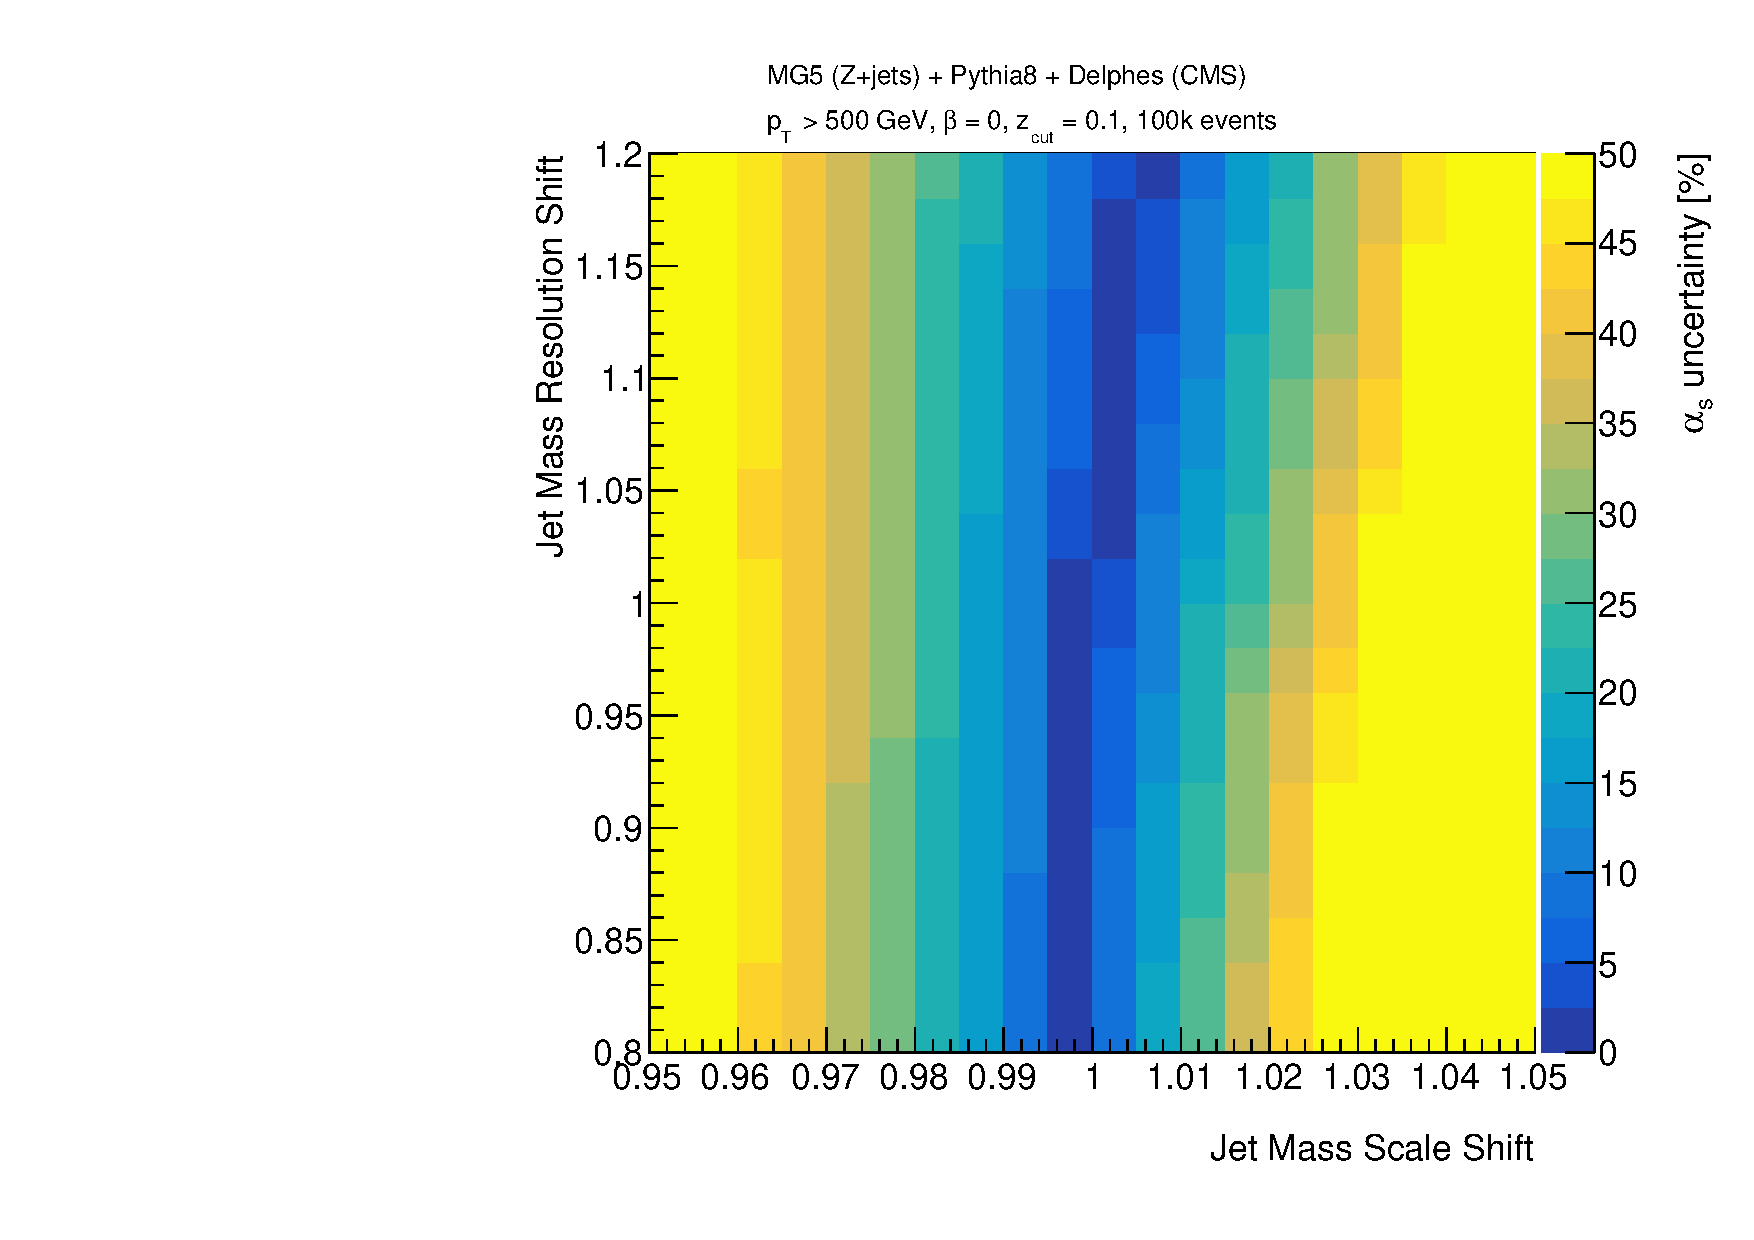
\includegraphics[width = 0.49\columnwidth]{figures/experimentaldemo/resolution_scan.pdf}
\end{center}
\caption{The impact of jet mass scale and jet mass resolution uncertainties on the uncertainty in the measured value of $\alpha_s$.  See the text for details.}
\label{fig:expfit}
\end{figure}

To understand the sensitivity to jet mass scale and resolution uncertainties, we conduct pseudo-experiments by sampling from the templates described in \Sec{sec:templates} and smearing with the migration matrix shown in the left plot of \Fig{fig:expres}.
%
We then unfold with another migration matrix that has the jet mass scale shifted or smeared by a fixed amount, and extract $\alpha_s$ via \Eq{eq:chi2fit} but for fixed and known $f_g=0$.
%
The results of this procedure are shown in \Fig{fig:expfit}.
%
There is little sensitivity to the jet mass resolution while there is a large uncertainty in the extracted $\alpha_s$ if the uncertainty in the jet mass scale exceeds a few percent.
%
Current jet mass scale uncertainties are below $5\%$ and resolution uncertainties are below 20\%~\cite{ATLAS-CONF-2017-063,CMS-PAS-JME-16-003}.
%
The mass scale uncertainty is as small as $2\%$ in various regions of phase space.
%
This again suggests that a $\sim 10\%$ measurement of $\alpha_s$ is feasible, as the uncertainty on the jet mass scale reaches the same level of maturity as the jet energy scale over the next few years.



\begin{comment}
\subsection{Fit in Pure Quark/Gluon Samples}

Fit Methodology:
	Which fix range (minimizing theory and experimental uncertainties)?
	Constraining quark vs gluon fraction (varying SD parameters)?
	Zeroth-order feasibility study
	
	Plot is for distribution folded over PDFs (can we get rid of that?)

	Choice of jet radius (varying resummation scale)

Assume (for this section) limited by experimental uncertainties



\subsection{Constraining Quark/Gluon Fraction with Data}

	Question:  constrain quark/gluon fraction (adjust $z_cut$)?
	Need to decide beta and zcut values
	Need to matching to fixed order
	beta = 0 mass is baseline
	
	
	Another study to mitigate quark/gluon fraction uncertainties
	Sensitivitity to PDF only to the extent of getting quark/gluon fraction
	Can mitigate that with fit.
\end{comment}



%%==============
%\section{Assessing Theoretical Uncertainties}
%%==============

%\input{sections/theoryuncerts}

%%==============
%\section{Alternative Observables}
%%==============

%\input{sections/alternatives}

%%==============
%\section{Estimated Sensitivity from Parton Showers}
%%==============

%\input{sections/partonshowerstudy.tex}

%%==============
%\section{Prospects at Lepton Colliders}
%%==============

%\input{sections/epluseminus.tex}

\clearpage

%%==============
\section{Conclusions and Future Outlook}
%%==============
\label{sec:future}
%\info{All}

In this paper we have performed a preliminary study of the possibility of performing an extraction of the strong coupling constant $\alpha_s$ from groomed jet substructure measurements at the LHC.  This has been made possible by recent advances in the calculation of groomed event shapes, which allow them to be resummed to NNLL accuracy, as well as advances in the understanding of the experimental uncertainties for groomed jet observables. 

We have highlighted a number of features that an extraction of $\alpha_s$ from groomed substructure would offer. In particular, the grooming procedure suppresses non-perturbative hadronization corrections to the distribution extending the range of perturbative control by a factor of $\sim 100$ as compared to the ungroomed case, where hadronization corrections are a dominant uncertainty. Furthermore, the nature of the non-perturbative corrections is completely different, and therefore a groomed extraction could provide complementary information. 

Using the groomed jet mass as a concrete example, we have performed a feasibility study for the extraction of $\alpha_s$ from groomed jet substructure. Taken separately, the groomed quark and gluon distributions both exhibit good sensitivity to $\alpha_s$. However, this study also highlighted a key issue relevant at the LHC. The leading behavior of the shape of the distribution is sensitive to the product $\alpha_s C_i$, where $C_i$ is the color Casimir, namely $C_A$ for gluon jets and $C_F$ for quark jets. This immediately implies that there is a degeneracy between the value of $\alpha_s$ and the quark gluon fraction of the sample. We highlighted two ways of overcoming this, either a fixed order calculation of the quark and gluon fractions, or the measurement of different observables, which enables a breaking of this degeneracy. Significantly better precision is achieved by the explicit calculation, however, this also introduces a dependence on the pdfs.

With currently achievable experimental and theoretical uncertainties, we have shown that an extraction of $\alpha_s$ at the $10\%$ level is feasible using the currently available data at the LHC.  We believe that this study motivates a serious effort to extract the strong coupling constant, $\alpha_s$ from jet substructure at the LHC using groomed jet shapes. A serious analysis will require advances on both the theory and experiment side. We therefore conclude by discussing some of the major obstacles that must be overcome.

%\ijm{Ben will say something about experiment}


On the theory side, we can separately discuss the three primary aspects of the calculation:

\vspace{5mm}

\noindent {\bf Resummation Accuracy:} For $e^+e^-$ event shapes, the current state of the art is N$^3$LL. This has been achieved only for a few select observables using the soft collinear effective theory. The extension  to N$^3$LL accuracy for the groomed jet mass would require only the calculation of the anomalous dimensions for the groomed soft function to three-loop. This could be performed using currently available techniques, and would enable N$^3$LL accuracy. 

At this level of accuracy it will also be important to asses perturbative power corrections in $\zcut$. While these have been shown to be numerically small in \cite{Marzani:2017kqd,Marzani:2017mva}, it would be good to achieve a better analytic understanding. 

\vspace{5mm}

\noindent {\bf Fixed Order Matching:} A key aspect, and potential complication to achieve a competitive theoretical accuracy as for $e^+e^-$ is the fixed order matching. For $e^+e^-$  the perturbative corrections to $e^+e^- \to$ 3 jets are known to NNLO \cite{GehrmannDeRidder:2007hr,Gehrmann-DeRidder:2007nzq,Weinzierl:2008iv,Weinzierl:2009ms}. To achieve a similar perturbative accuracy for the matching for the groomed jet mass will require $2\to 3$ matrix elements at NNLO. While results for the amplitudes are just becoming available \cite{Gehrmann:2015bfy,Dunbar:2016aux,Badger:2013yda,Badger:2017jhb,Abreu:2017hqn}, it will be a while before numerically efficient evaluations of the relevant cross sections are available. We believe that this is currently the theoretically most difficult ingredient. 

\vspace{5mm}

\noindent {\bf Non-Perturbative Corrections:} Finally, in addition to improving our understanding of the perturbative accuracy of the observable, it will also be crucial to improve our understanding of the non-perturbative aspects of groomed observables. While it has been shown through Monte Carlo studies that non-perturbative effects are suppressed throughout a large component of the distribution, it will be important to quantify this further. In the case of $e^+e^-$ event shapes, operator definitions of soft matrix elements allow for field theoretic definitions of the non-perturbative parameters. Ideally this could also be performed for groomed observables, placing the groomed jet mass on a firmer theoretical footing.

\vspace{5mm}

Experimentally, there are three broad topics that need to be addressed for a precision extraction of $\alpha_s$:

\vspace{5mm}

\noindent {\bf Mass Scale Uncertainties:} At the moment, ATLAS~\cite{Aaboud:2017qwh} and CMS~\cite{CMS-PAS-SMP-16-010} have very different approaches for determining the jet mass scale uncertainty, both with known limitations.  CMS performs a fit to the hadronic $W$ boson mass peak in one-lepton $t\bar{t}$ events and takes the shift in the peak position as the uncertainty in the jet mass scale (which is negligible and thus ignored)~\cite{Sirunyan:2016cao}.  Two challenges with this approach are that (a) the peak position is a convolution of particle-level and detector-level effects and (b) it is not clear that uncertainties derived for boosted $W$ bosons should be the same as for generic quark and gluon jets at all masses.  One can overcome (a) with a technique like forward-folding~\cite{ATLAS-CONF-2016-008,ATLAS-CONF-2016-035}.  Various PS MC generators are studied, but it is likely not sufficient to have one global model comparison.  The impact on the jet mass resolution in one topology may be completely different than the impact of the scale, resolution, or acceptance in another topology.  In contrast, the ATLAS measurement propagates constituent-based uncertainties through to the groomed mass.  These uncertainties are derived from matching tracks to calorimeter-cell clusters and studying the energy and angular matching.  Studies have shown that this `bottom-up' approach works well for reproducing the jet energy scale~\cite{Aaboud:2016hwh}, which has been validated also for groomed jets in Ref.~\cite{Aaboud:2017qwh}.  However, this does not hold exactly for the mass, which is not linear in the constituent energies~\cite{Nachman:2016qyc}.   The uncertainties are validated using the standard ATLAS approach using track-jets~\cite{Aad:2013gja,ATLAS-CONF-2017-063}, but to achieve higher precision, a more detailed understanding of the impact of energy thresholds, fluctuation correlations and calorimeter cluster merging will be required.

\vspace{5mm}

\noindent {\bf Mass Resolution Uncertainties:} ATLAS and CMS use the same approaches for the resolution as for the scale (bottom-up and $W$ mass peak).  ATLAS validates their approach in a similar manner as CMS, by using the $W$ mass peak from $t\bar{t}$ events\footnote{This validation does not have the same complete forward-folding machinery as was used by ATLAS for trimmed jets.}.  The mass resolution is mostly not the limiting factor, but it could be if the situation is not improved as the jet mass scale precision improves. 

\vspace{5mm}

\noindent {\bf Pileup Modeling and Mitigation:} Grooming significantly reduces the impact of pileup, but if the Run 3+ data are to be used (pileup levels of 80+), then a significantly better and more detailed understanding of the degradation due to pileup will be required.  Statistical are currently not dominant, so it is conceivable that the higher instantaneous luminosity data is not used for the precision $\alpha_s$ extraction.  This may change if one wants to exploit the largest lever-arm possible; to access the highest $p_\text{T}$ jets, we will need more data.

\vspace{5mm}

It would also be interesting to study in more detail the use of other groomed observables. Since it may be the case that it is ultimately experimental uncertainties that are the limiting factor, one potentially interesting direction is the use of track based measurements. From the experimental perspective, this significantly reduces uncertainties, particularly in a high pile up environment. From the theoretical side, it introduces the need for non-perturbative track functions. However, for specific observables, only certain moments of the track functions are required. This therefore offers the potential that combined fits for the moments of the track functions and $\alpha_s$ could be performed, much like how fits are performed for $e^+e^-$ event shapes. Significantly more theoretical work is required to see if this is truly a viable possibility, although we believe that this is well motivated.


We are optimistic that these difficulties on both the theory and experiment side can be overcome, enabling a precision probe of the strong coupling constant from jet substructure in the LHC environment.

\begin{acknowledgments}

The work of GS is supported in part by the Paris-Saclay IDEX under the
IDEOPTIMALJE grant, by the French Agence Nationale de la Recherche,
under grant ANR-15-CE31-0016, and by the ERC Advanced Grant Higgs@LHC
(No.\ 321133).
%
The work of JT is supported by the DOE under grant contract numbers DE-SC-00012567 and DE-SC-00015476.
%
IM and BN are supported in part by the Office of High Energy Physics of the U.S. Department of Energy under Contract No. DE-AC02-05CH11231, and the LDRD Program of LBNL.

\end{acknowledgments}

\bibliographystyle{jhep}
\bibliography{lh2017_alphas}

\end{document}
